\documentclass[pdftex,11pt,a4paper]{book}
\usepackage{ujthesis,enumerate,amssymb,amsmath}
\usepackage{cite,graphicx}
\usepackage[nottoc]{tocbibind}
\linespread{1.2}
\dissertation
\coverFont{\large}
\setlength{\parskip}{0.5ex plus0.5ex minus0.2ex}
\setlength{\spaceLength}{7mm}
\approvedtitle{Particle Swarms and the Frequency Assignment Problem}
\student{William Bezuidenhout}
\degree{Magister Scientiae}
\field{Information Technology}
\faculty{Faculty of Science}
\supervisorName{Dr. G.B. O'Reilly}
\submissionDate{June 2010}
\begin{document}
\makecover
\tableofcontents
\part{Background}
\chapter{Introduction}
\section{Introduction}
In the technology age, life is almost unfathomable without the mobile phone. It is hard to believe how the business world managed to function in the pre-mobile phone era\footnote{Pre 1980s where the mobile phone did not yet exist}. 

The invention of the mobile phone fulfilled the need to always be connected and be within reach of the modern world. This need can actually be attributed to feeling part of something and this something is deemed as being part of a network. This is similar to how mobile phones are able to provide connectivity at almost any location within a country.

Behind the connectivity of mobile phones lies an intricate layer of communication technology which has evolved since the invention of the normal landline phone. This technology is referred to at the top level as wireless communication, which includes inventions such as the radio. To enable communication at the level needed by mobile phones, wireless communication had to evolve and go a step further than normal radio communication. Hence the concept of cellular mobile networks was developed.

Without cellular networks mobile phones have no means of providing communication. The purpose of the cellular network is to provide the necessary functions to connect and facilitate communication between two entities (mobile phones) over a wireless network. 

Cellular networks achieve this level of communication through expensive equipment and ``smart'' algorithms. By ``smart'' algorithms, what is actually meant is algorithms that utilise artificial intelligence concepts to perform a certain function in an attempt to either automate a task within the network or improve a certain part of the network. Therefore, the correct term for these types of algorithms is actually artificial intelligence (AI) algorithms.

AI algorithms have a wide spread of functions that they can perform ranging from making informed intelligent decisions to optimising the operation of certain processes. In particular computers are indeed very apt at optimising certain procedures. This is because a computer is able to test and evaluate a huge number of different alterations and combinations of a certain procedure in a short amount of time, thereby allowing it to find the best combination out of those tested.

In this dissertation an algorithm is presented which concentrates on cellular phone networks. This particular algorithm falls into the latter part of the AI algorithms discussed, namely an AI optimisation algorithm. Thus the algorithm presented in this dissertation operates on a cellular phone network to optimise a certain part of the network.

In this section a introduction was presented to the dissertation. The main themes of the dissertation were outlined namely, cellular phone networks and optimisation algorithms. In the next section research plan and chapter breakdown is presented which is followed by this dissertation.
\section{Research Questions and Objective}
As previously discussed, an artificial intelligent algorithm is presented in this dissertation that generates plans for use by cellular networks. The purpose of creating such an algorithm is to determine the applicability of modern swarm-based algorithms with regard to finding better solutions to real-world problems that exist in domains such as cellular communication.

The research approach followed in this dissertation was first and foremost to understand the cellular network domain. More importantly, the focus is on how and what frequencies are used to facilitate communication as well as what affects the quality of the communicational link between two entities in a cellular network. 

The cellular domain is the problem domain, but to develop a solution in the problem domain a study needs to be conducted in the artificial intelligence domain, namely a study of optimisation algorithms. In order for a new optimisation algorithm to be developed, other algorithms that have achieved success in the respective optimisation problem domains in which they have been applied need to be investigated.

Therefore in an attempt to develop and apply a modern viable optimisation-based algorithm, a series of research questions has been identified which need to be answered. The research questions are as follows:
\begin{itemize}
\item \textbf{Question 1} --- What is cellular technology, how it got developed and what improvements have been made since its initial development?
\item \textbf{Question 2} --- What is the architecture behind a modern cellular network, how do the various hardware entities within a network communicate with each other and how is a communicational link established between two users of the network?
\item \textbf{Question 3} --- What exactly is the frequency problem and how does it affect modern wireless communication?
\item \textbf{Question 4} --- What variants of the frequency problem exist and which are most applicable to cellular networks?
\item \textbf{Question 5} --- What are the most popular optimisation algorithms and what characteristics make them unique?
\item \textbf{Question 6} --- With algorithms that achieved success in their respective optimisation problems, what particular technique is used by the algorithms that allowed them to achieve better performance?
\end{itemize}

The PSO algorithm might be short and elegant, but applying it to the FS-FAP required various new techniques in response to the following questions:
\begin{itemize}
\item How can a particle best be represented as a frequency plan?
\item How can one frequency plan move to another?
\item How can particles be prevented from using forbidden frequencies when they fly towards a particular plan?
\end{itemize}

The above questions were only the preliminary questions and were in fact a problem that had to be addressed for successful application of the PSO to the FAP. In chapter~\ref{chpt:psoapplicationFAP} a discussion is presented on how these problems were solved as well as how other problems were solved that were not anticipated.

Throughout the course of this dissertation the aim is to answer each of these identified research questions. In the next section a chapter breakdown of this dissertation is presented.

The aim of this dissertation is first and foremost to answer the identified research questions. Answering these questions will aid in reaching the research objective of this dissertation. The research objective is therefore to develop and determine the viability of an algorithm based on modern swarm optimisation techniques that will operate on the frequency assignment problem in an attempt to provide better frequency plans for use in cellular networks.

\section {Chapter Breakdown}
\subsection{Part I - Background}
The first part of this dissertation is concerned with the domain and problem the algorithm presented in this dissertation addresses, and finally to also understand the intricate details of how the algorithm operates.

Below is an outline of the chapters in the first part of this dissertation.
\subsubsection{Chapter 1}
This chapter provides an introduction to the dissertation as well as a broad overview of the topics in the dissertation will discuss.
\subsubsection{Chapter 2}
This chapter is concerned with providing information on how a modern cellular network functions. Within this chapter a brief history is presented on how cellular network technology was developed. The chapter also provides an overview of the architecture of a cellular network,and each part of the network's intended purpose and function to facilitate wireless communication is discussed.
\subsubsection{Chapter 3}
This chapter presents the problem that the dissertation addresses, namely the frequency assignment problem. The chapter provides a discussion on why the problem exists, the causes of the problem and what it means for a problem to be NP-Complete. Furthermore the variants of the problem and how they differ depending on the wireless domain that is being considered are alos discussed. Finally the chapter also provides a formal definition of the problem which is later utilised by the algorithm developed in this research.
\subsubsection{Chapter 4}
This chapter marks the beginning of a discussion on various optimisation algorithms in this dissertation. The algorithms presented in this chapter were chosen due to their widespread usage as well as success on NP-Complete problems. Each algorithm is discussed in depth providing an outline of the core features that make the algorithm unique as well as each core feature in detail. For each algorithm the chapter also presents an analysis on related work of the particular algorithm being applied to the frequency assignment problem. 
\subsubsection{Chapter 5}
This chapter is concerned with providing algorithms that are new in the research domain of optimisation algorithms. The algorithms presented in chapter 4 are fairly old and have been applied to a wide variety of problems. Algorithms in this chapter are relatively new in the optimisation domain and have not been applied to the same number of problems as the algorithms in chapter 4. In this chapter swarm algorithms are presented and the algorithms have the particular characteristic that they are based generally on processes observed in nature. Each algorithm is discussed in depth with its core characteristics outlined. Furthermore for each algorithm an analysis is given if the algorithm were to be applied to the frequency assignment problem. Finally it is formally stated what algorithm this dissertation is applied to the frequency assignment problem in this research.
\subsection{Part II - Implementation}
\subsubsection{Chapter 6}
This chapter provides a discussion of the algorithm developed to be applied to the frequency assignment problem. Within this chapter an outline is given of the process in developing a specialised particle swarm algorithm for the frequency algorithm. Each specialised technique developed is discussed in depth, along with an explanation of why the technique is needed as well as why it is used by the algorithm.
\subsubsection{Chapter 7}
This chapter is concerned with providing the results after applying the algorithm to a specialised set of benchmark problems for frequency assignment algorithms. The particular selected benchmark problems were discussed in chapter 2.
\subsubsection{Chapter 8}
This chapter concludes this dissertation. In this chapter it is determined whether the research goal was reached as well as whether any future work can be done to improve the presented algorithm.
%Introduction
\chapter{Cellular Technology}
\section{Introduction}
In the information age we currently live in almost every device has some sort of wireless technology it uses to provide a specific service. Radios for audio entertainment; Television remotes to change 
channels; Cellular phones for communication; Wireless access points to create wireless LAN's\cite{Karen2004}. Wireless technology is now part of our everyday life.

The popularity and rapid adoption of wireless technology hasn't been kind to the management, planning and operation of wireless networks; It has actually worsen a problem known as the Frequency Assignment problem (FAP) which is present in all forms of wireless communication especially in GSM Cellular networks.

In this chapter we will start of by giving a brief history of the Frequency Assignment Problem. After the brief history overview we will give a description of the problem and explain some of the
underlying concepts needed to understand the Frequency Assignment Problem. We will then move on to discuss the different variants present in the current domain. Further more we will
then discuss the two underlying approaches used in solving the Frequency Assignment Problem (FAP).
\section{GSM Networks}
The General System for Mobile Communications (GSM) is a system for multi-service cellular communication which is capable of providing voice as well as data services. Most cellular networks in operation 
are GSM based. The primary service that GSM caters for is voice communication, but other data services such as Short Message Service (SMS), Multimedia Message Service (MMS) and Internet 
connectivity services such as GPRS are becoming more important\cite{Eisenblatter}.

GSM is one of the most widely used radio communications technologies, which is why we need to look at the history behind it in order for us to understand the domain of radio communication better.We will now present a brief history of the GSM network specification.
\subsection{A Brief History of GSM Networks}
In the early 1981 a group known as the Groupe Speciale Mobile (GSM) was established to develop a Europe wide radio communication system using the reserved 900 MHz band\footnote{In 1990 the United Kingdom requested that 1800MHz band be added to the scope of the GSM standard group. This variant of the GSM specification became known as the \emph{Digital Cellular System 1800} (DCS1800) \cite{GSM92}.}.

At the start of the GSM specification in the early 1980's it was initially thought that the system would be analogue based, but this soon changed with the \emph{Integrated Service Digital Network} (ISDN) specification nearing completetion. As such the GSM specification started following much of the same design principles and access protocols that ISDN exhibited. After the completion of the ISDN specification and the advantages it brought to the field, it became unofficially clear that GSM would be based on digital transmission and that speech would be represented by a digital stream of 16 kbits/s \cite{GSM92}.

Before the switch to digital transmission was finalized the GSM first wanted to evaluate the spectral efficiency of analogue and digital based transmission. Spectral efficiency plays an important part in wireless communication since the radio spectrum is a limited resource and whichever transmission technology is used, should maximise the utilization of the spectrum. Maximum utilisation is an important problem which we will discuss in detail in later sections of this chapter. The Spectral evaluation was conducted over a period of 3 years from 1984-1987. In 1987 a report was published about the 3 year evaluation and subsequently it became official that the GSM system would be digital based using \emph{Time Division Multiple Access} (TDMA) \cite{GSM92,GSMSysEngin}.

By the early 1990’s GSM became an evolving standard and the first GSM based network was demonstrated in 1991\footnote{Near the end of 1991 the GSM group was renamed to \emph{Speciale Mobile Group} (SMG) to eliminate confusion with the standard and the group.}. The following year a number of GSM networks were operating in Europe due to mobile terminals / equipment capable of operating on the networks becoming more widely available to the general public. In the same year an operator in Australia became the first non-European operator to implement a GSM based network\cite{Eisenblatter}.

The collective subscriber base of GSM networks surpassed the million subscriber mark in 1993. Due to this phenomenal growth in GSM network use, numerous extensions were made to the GSM specification. 
Some of the extensions that were made are the following\cite{Eisenblatter}:
\begin{itemize}
\item Half rate speech telephony
\item Improved SMS
\item Line Identification
\item Call waiting
\item Call holding
\end{itemize}
The specification with these extensions defined is known as the GSM Phase 2. As the world shifted towards more digital and data intensive services it became difficult to deliver these services over GSM 
networks. This difficulty was due to the restriction that data could only be transmitted at 9.6 Kbps. A move to eliminate this restriction was made with the specification of GSM Phase 2+. 

The new specification defined new technologies such as General Packet Radio System (GPRS) and \emph{Enchanced Data rate for GSM Evolution} (EDGE) which were designed with the primary goal of making more bandwidth available for data transmission.
These new technologies have an inherent requirement that there be a higher signal to noise ratio present at transceivers. This requirement has an impact that effects radio interfaces and more 
importantly Frequency planning \cite{Eisenblatter}. 

The actual signal to noise ratio at a receiver is dependent on a number of factors that include \cite{Karen2004}:
\begin{itemize}
\item Frequency used at the transceiver
\item Strength of the signal
\item Weather conditions
\item Shape of the surrounding environment
\item Direction of the transmission
\end{itemize}
Even taking these factors into account the calculation of the signal to noise ratio at a transceiver is not trivial. For a more in depth discussion on the calculation the reader is directed at the survey by \cite{Karen2004}.

As the GSM standard matured as a cellular technology, industry experts already began specification of the next generation of cellular networks which would in time, replace the GSM cellular system. The specification of a new standard is considered to be a natural evolution of the technology. Each standard is designed with specific use cases in mind as to what its users might want to do as well as what is possible with the technology at the designers disposal. As time goes by, the technology improves and users habits and needs change, thus the standard must be improved upon to serve these new needs and incorporate new technology.

The \emph{Universal Mobile Telecommunications System} (UMTS) can be considered the 3rd generation (3G) of cellular networks. UMTS was designed from the beginning to operate in parallel with the legacy GSM system. This decision was made to make the deployment of the system as hassle free as possible for the network operators. The first standard of the UMTS was issued in the beginning of 2000 and subsequently most modern networks are based on it or are migrating their networks to it.

UMTS is a large improvement of the GSM in two areas namely Data Transmission bandwidth and Frequency Planning due to UMTS utilising \emph{DS-CDMA} (direct sequence code division multiple access) and \emph{WCDMA} (Wide Band Code Division Multiple Access). The higher data transmission speed (2 Mb/s) can be attributed to UMTS using the DS-CDMA scheme. The scheme also allows more users to be served than previous generation of networks. A direct consequence of WCDMA which sends information over a wide-band of 5 MHz is that no frequency planning problem comparable to that of GSM has to be solved\cite{tabuglobalplanning3g,Eisenblatter}.

In this section we gave a brief overview of the history of the GSM Network specification. In the next section we will present an explanation of the topology of GSM network as well as look at the 
underlying problems present in a GSM networks.
\subsection{Topology of a GSM Network}
GSM networks consists of a variety of different subsystems to realise the goal of establishing a radio communication link between two parties. The hierarchy of systems and their respective connections to
each other is illustrated in figure 1. We will now briefly explain each subsystem.
\subsubsection{Mobile Station (MS)}
A Mobile station (MS) as it is defined in the GSM spec refers to any mobile device that is capable of of making and receiving calls on a GSM network.  The MS is the main gateway 
for a user to gain access to the GSM network. The MS has two features which play an important role throughout the GSM Network, namely:
\begin{description}
\item[Subscriber Identification Module (SIM)] --- Usually inserted into a mobile devices. The SIM contains the \emph{International Mobile Subscriber Identity} (IMSI) and is used throughout the network 
for Authentication as well as being a key part in providing encrypted transmissions.
\item[International Mobile Equipment Identity(IMEI)] --- Used to identify mobile station equipment. Primarily used in the denial of service to equipment that has been blacklisted\footnote{Equipment can be blacklisted for a variety of reasons e.g. theft} and tries to gain access to the network.
\end{description}
The MS has the capability to change the transmission power is uses from its base value to a maximum value of 20 mW. The change in transmission power is automatically set to the lowest level by the Base Transceiver Station to ensure reliable communication after evaluating the signal strength as measured by the MS \cite{GSMSysEngin}. % The power adjustment also minimizes cochannel interference, which we can talk about later when we introduce interference

\subsubsection{Base Station Subsystem (BSS)}

According to the GSM Phase 2+ specification this system is viewed by the \emph{Mobile Switching Centre} (MSC) through an Abis radio interface as the system responsible for communicating with Mobile Stations in a particular location area. The BSS usually consists of one \emph{Base Station Controller} (BSC) with one or more \emph{Base Transceiver Stations} (BTS) which it controls. The communication link between the MSC and BSC is the called the A-interface and the communication link between the BSC and BTS is called the Abis interface. The definition of these communication interfaces is beyond the scope of this disseration, the interested reader is directed to the book \emph{GSM System Engineering} by Asha Mehrotra. A BTS has similar equipment to that of a Mobile Station. Both have transceivers, antennas and the necessary functions to perform radio communication. 

In a GSM network the Service Area (SA) is subdivided into Location Areas(LA's) which are then futher divided into smaller radio zones called cells \cite{GSMSecurInTeleNetwork}. A cell is served by only one BTS and is usually regarded to be in the center of a cell. Even though cells are modelled as being hexagons (See figure 3) the actual coverage area of a cell has no predefined regular shape. Futhermore a cell is divided into 1 to 3 service sectors and each sector is allocated an antenna/transceiver \cite{GSMSysEngin}. Depending on how many sectors are at a cell, the operating angle of the antennae needs to be adjusted accordingly to ensure 360 degree service. If there is only one sector an omni-directional antenna is used, otherwise the antennae operating angle are adjusted to $\frac{360\,^{\circ}}{n}$ where ${n}$ is the amount of antennae \cite{Eisenblatter}.

Each sector operates one or more elementary transceivers called TRX’s. The amount of TRX’s per sector is determined by the expected peak traffic demand that the cell must be able to handle. Each TRX can handle 7 to 8 communication links or calls in parallel except the first TRX, which handles fewer calls than normal due to it being responsible for transmitting cell organisation and protocol information \cite{Eisenblatter}. TRX’s are able to handle 7-8 calls in parallel due to the use of \emph{Frequency Division Multiplexing} (FDM) and \emph{Time Division Multiplexing} (TDM) schemes. TRX’s are assigned channels which enable them to provide conversion between digital traffic data on the network side and the radio communication between Mobile Stations and 
the GSM network. \cite{ACOvsEA,FAPOrientationModel}

\subsubsection{Mobile Switching Centre (MSC)}

The MSC is at the heart of cellular switching system and forms part of the \emph{Network Switching Subsystem} (NSS). The MSC is responsible for the setting up, routing and supervision of calls between GSM subscribers. The MSC has interfaces on the one side to communicate with GSM subscribers (through the BSS) and on the other it has interfaces to communicate with external networks. The MSC interfaces with external networks to utilise their superior capability in data transmission as well as for the signalling and communication with other GSM entities \cite{GSM92}. 

The most basic functions that an MSC is responsibile for in a network are the following \cite{wirelesstelcoMullet}:
\begin{itemize}
\item Voice call initialization,routing,control and supervision between subscribers.
\item Handover process between two cells.
\item Location updating.
\item MS authentication.
\item SMS delivery.
\item Charging and Accounting of services used by subscriber.
\item Notification of other network elements.
\item Administration input or ouput processing functions.
\end{itemize}

To achieve most of these functions the MSC has an integrated \emph{Visitor Location Register (VLR)} database that stores call setup information for any MS that is currently registered for service with the MSC \cite{GSM92,wirelesstelcoMullet}. 

The VLR retrieves this information from the \emph{Home Location Register (HLR)} which contains all the registered GSM subcriber information for the network. This information enables the MSC to quickly retrieve the nesaccery information to setup a call between two entites \cite{GSMSysEngin,GSMSecurInTeleNetwork}.

A requirement for being able to communicate with other network elements such as \emph{Public Switching Telephone Networks} (PSTN) is the ability to multiplex and demultiplex signals to and from such network elements. This operation is a necacity, since the incoming or outgoing connection bitrate from the source entity might either be to low or to high for the receiving entity.

A typical scenario where this operation proves vital is when a mobile subcriber makes a call to a subcriber on a PSTN. The connection bit rate needs to be changed at the MSC from a wireless connection bitrate to a bitrate suitable for transmission over a PSTN.

\subsubsection{Network Databases}
The HLR, AUC (Authentication Center) and EIR (Equipment Identity Register) are the 3 'back-end' databases which stores and provides information for the rest of the GSM Network. We will now briefly discuss what the purpose of each database is and its core functions.

\paragraph{Home Location Register (HLR)}
The HLR is a database that permenantly stores information pertaining to a given set of subscribers. The HLR needs to store a wide range of subcriber parameters because it is the reference source for anything GSM subscriber related in the network. 

Subscriber parameters that are stored in the database include: Billing information, routing information, identification numbers, authentication parameters,subscribed services. The following information is also stored but the information is of a temporary nature and can change at anytime: Current VLR and MSC the subscriber is registered with; Wheter the subscriber is roaming \cite{GSMSysEngin}.

\paragraph{Authentication Center (AUC)}
The Authentication center is the entity in the GSM network that performs security functions and thus stores information that enables it to provide secure over the air communication. The information that is stored contains authentication information as well as keys that are used in ciphering of information.

During an authentication procedure no ciphering key is ever transmitted over the air, instead a challenge is issued to the mobile who needs to be authenticated. This callenge requires the mobile station to provide the correct \emph{Signed Response}(SRES) with regard to the random number generated by the AUC. The random number and ciphering keys that are used change with each call that is made, thus an attacker would gain nothing by intercepting a key, since it will change with the next call \cite{GSMSysEngin}.

Each mobile that is registered in the HLR database needs to be authenticated and each call that is instansiated needs to retrieve keys from the AUC to establish a secure communication link. The AUC is sometimes included with HLR to allow for fast communication between the two entities \cite{GSMSysEngin}.

\paragraph{Equipment Identity Register (EIR)}
The EIR is a database that stores the IMEI numbers of all registered mobile equipment that has accessed the network. Only information about the mobile equipment is stored, nothing about the subscriber or call is stored in the database.

Typically there is only one EIR database per network and interfaces to the various HLR database contained in the network. The IMEI's are grouped into 3 categories: \emph{White List}, \emph{Black List} and the \emph{Gray List}. The White list contains only the IMEI numbers of valid MS's; the Black List stores the IMEI numbers of equipment that has been reported stolen and the Gray List stores the IMEI numbers of equipment that has some fault (faulty software, wrong make of equipment).

\subsubsection{GSM Network Management entities}
In a GSM network most of the elements that form part of and make the network function are often distributed in a wide geographical area to provide the best network converage for the customer. 

For a network to function properly and efficiently network engineers need to be kept up to date on the state of the network and be alerted if \emph{any} problems occur. For this purpose there exists two systems in the GSM network architecture that allows for this functionality required by network engineers. 

The one system is called the Operations and Management center which is responsible for centralized regional and lcoal operational and maintenance activities. The other system called the Network Management System unlike the OMC provides global and centralized managemenent for operations and maintenance of the network suppored by the OMCs \cite{GSMSysEngin}.

We will not discuss the OMC and NMC in a bit more detail where we'll define the most critical functions they peform.

\paragraph{Operational and Managemenet Center}
The OMC is capable of communicating with GSM entities using two protocols namely SS7 and X.25. The SS7 protocol is usually used when the OMC is communicating within the GSM network over short and medium distances. The X.25 protocol is used for large external data transfers. All communication where the OMC is involved typically occurs over fixed line networks and/or leased lines. The OMC is usually used for day to day operation of a network \cite{GSMSysEngin}.

The OMC has support for alarm handling. An alarm in a GSM network goes of whenever a predefined expected condition does occurs. Engineers are able to define the severity of an alarm which defines who and what is futher alerted when and if the alarm is escalated to a higher level \cite{GSMSysEngin}.

To give one an idea of when and why and alarm goes of consider the following scenario: The MSC controls a set of BSS systems. Now for some reason a certain region experiences a power blackout. All the BSS affected by the blackout switch over to reserve power if availble. A first alarm is sounded to let the engineers / network know that the BSS is using reserve power. When the BSS reserve power is depleted the MSC sounds an alarm letting the network know that a specific BSS cannot be contacted.

Typically in the above scenario the severity of the first alarm will be of a medium priority. The second alarm is much more serious and its severity will be of a high priority.

The OMC is also capable of fault management in the GSM network. The OMC is able to activate,deactivate,remove and restore a service manually or automatically of network devices. Various tests can be run as well as diagnostic information can be retrieved on the network devices to detect any current or future defects \cite{GSMSysEngin}.

\paragraph{Network Management Center}
The NMC is similar to the OMC but it is not restricted to only regional GSM entities as it is in charge of the all GSM entities in the network. The NMC provides traffic management for the global network and also monitors high priority alarms such as overloaded or failed network nodes. It is usually used in long term planning of a network, but it has the capability to perform certain OMC functions when an OMC is not staffed. 

\subsection{GSM Network problems}
\section{The Frequency Assignment Problem}
The Frequency Assignment Problem (FAP) is a generalisation of the graph-colouring problem and is subsequently an NP-hard problem. This is because one has a finite amount of frequencies which needs to be 
assigned to antennae/transceivers (TRX's)  where the amount of transceivers to be assigned frequencies greatly out weigh the amount of available frequencies. Thus it is inevitable that a network will 
have interference and we can only minimise the amount of interference that might occur on the network - an optimisation problem. 

A contributing factor to the difficulty of the FAP is due to the scarcity of usable frequencies in the radio spectrum, which forces network operators to reuse their allocated/licensed frequencies in their respective networks. The scarcity of the usable frequencies in the spectrum can be attributed to the overuse of certain bands as well as large scale reuse of frequencies in networks. This has put strain on the spectrum and has complicated the management of networks significantly because interference is more likely to occur.

\subsection{Interference}
Interference occurs when frequencies assigned to connections differ by a small margin. The amount of inference on a connection defines the quality of service. One can naturally make the deduction that 
the more frequencies differ used on connections in a area, the better quality of service one will experience in that area. Cellular networks use the amount of interference on their networks as 
qualitative measure for their \emph{Quality of Service} (QoS). A network with high interference would experience a lot of dropped connections, which occurs when the interference is too high to sustain a connection for communication.

Primarily Interference occurs if the Electromagnetic constraints are violated, which are defined as:
\begin{description}
\item[Co-Cell] ---
\item[Adj Channel] ---
\item[Co-Site] ---
\end{description}
A fourth constraint, namely the Handover constraint is also applicable in Cellular networks which we will discuss in section 4.

\subsection{Frequency Assignment Types}
Within the FAP domain there are  a variety of sub problems which originated over the decades of which wireless communication has survived through. We will discuss the most popular problems found in the literature over the last few years in Section 2. The FAP can be classified into two categories:
\begin{enumerate}[\bf{(}a\bf{)}]
\item \emph{Fixed Frequency/Channel Assignment} (FFA/FCA) is the process of permanently assigning frequencies to cells (cellular towers). The frequencies assigned are fixed and cannot be changed on the fly while 
the network is active , since the frequencies assigned to the cell form part of a delicate frequency plan designed to keep interference to minimum.
\item \emph{Dynamic Frequency/Channel Assignment} (DFA/DCA) is the process of allocating channels to cells as they require it to meet the current traffic demand imposed on them by clients. 
\end{enumerate}
Each cell can be assigned multiple frequencies based on the amount of transmitters or TRX's it has. The amount of TRX's in a cell depends on the expected amount of traffic the particular cell must 
handle.

Most of the research in the FAP has concentrated on the FFA. The reason for this is because FFA is a static technique, which allows it to come up with a better solution since it has more time for 
calculation. FFA is also easier to implement in practise and allows the network operators to cater for the worst case scenario - heavy traffic load on the network. The DFA is at the moment a very hard 
problem because the network frequency plan is constantly changing, which means as the traffic on the network increases the longer the DFA focused algorithm will take to allocate a frequency. This 
increase in processing time is because the algorithm has to take into account more constraints with a lower available frequency pool. DFA must do this process within seconds since a cell needs to serve clients. Most researchers have concentrated on solving the FFA using heuristic approaches like neural networks, local search techniques and more recently meta heuristic approaches which include genetic algorithms, simulated annealing , ant colony optimisation and particle swarm optimisation.

In this section we have given a description of the Frequency Assignment Problem and introduced some concepts which we will use throughout the dissertation. In the next section we will present the 
Mathematics that govern the Frequency Assignment Problem.
\subsection{Mathematical Formulation}
\subsection{Types of Frequency Assignment Problems}
\subsubsection{Minimum Order Frequency Assignment Problem}
\subsubsection{Minimum Span (MS) Frequency Assignment Problem}
\subsubsection{Fixed Spectrum (FS) Frequency Assignment Problem}
\subsection{Frequency Assignment Models}
\subsubsection{Binary Constraints}
\subsubsection{Cost Function Minimisation}
\section{Summary}
%GSM Cellular Networks
\chapter{The Frequency Assignment Problem}
\label{chpt:fap}
\section{Introduction}
The \glsreset{FAP}\gls{FAP} is a generalisation of the graph-colouring problem and is consequently an NP-Complete problem\cite{FAPRAMColouring}. The \gls{FAP} is an NP-Complete problem due to fact that only a finite number of frequencies can be assigned to \glspl{TRX}, where the number of transceivers to be assigned frequencies greatly outweighs the number of available frequencies\cite{FAPRAMColouring}. A more thorough definition of what it means for a problem to be NP-Complete is given in section~\ref{sec:NPComplete}.

In wireless communication a huge concern is interference, which occurs when, frequencies used for communication are close to each other in the frequency spectrum\cite{Karen2004}. Interference and its effects are discussed in detail in section~\ref{sec:Interference}. Essentially for the \gls{FAP} the primary concern is to develop an approximate plan on assigning frequencies in such a way that interference is kept to a minimum. 

Using exact algorithms to find a solution is not practical since the time to find a solution is polynomial. Generally metaheuristic algorithms are used to find optimal solutions to NP-Complete problems\cite{ACOvsEA}. Chapter~\ref{chpt:heuristic} presents a discussion on algorithms that are used to find solutions to NP-Complete problems. 

As discussed in chapter~\ref{chpt:celltech}, network operators are licensed a range of frequencies from the available spectrum. A licensed piece of spectrum contains a series of consecutive frequencies as well as gaps. Gap frequencies are barred from being used by any device within the network as they may have already been allocated to another operator for use \cite{FAPInCell}. By barring frequencies, a scenario is avoided where the different networks' equipment interferes with their respective operations\cite{FAPInCell}.

Due to the whole spectrum not being available to network operators and only a subset being available for commercial communication as per the frequencies allocated to them, networks opt to reuse their frequencies\cite{FAPInCell}. The networks do this to maximise the use of their allocated frequencies and to minimise their licensing fees, since if the network needs more frequencies, they need to be licensed\cite{FAPRAMColouring}.

It is not always possible to simply allocate more frequencies to a network even if the network pays the associated fees. The whole commercial spectrum may already have been licensed to various entities. Hence, licensed frequencies are a very valuable and scarce commodity \cite{FAPRAMColouring,FAPInCell}.

The chapter is organised as follows. The first section presents a discussion on NP-Complete problems. In section~\ref{sec:chm} constraint handling mechanisms are presented. Section~\ref{sec:FreqAssignmentTypes} presents an overview of different methods for allocated frequencies. Interference is discussed in depth in section~\ref{sec:Interference}. After the interference discussion a section is presented on the different types of frequencies assignment problems in section~\ref{sec:FAPVariants}. A mathematical formulation of the fixed spectrum frequency assignment problem is presented in section~\ref{sec:FAPMathDef}. Section~\ref{sec:FAPBenchmarks} provides an overview of the different benchmarks used to evaluate frequency assignment problems. After the discussion on the different benchmarks that are available in the domain a section on where the FAP is encountered in the industrial domain is presented. 

This chapter concludes with a section that summarises the contents presented. The next section presents an overview of what it means when a problem is NP-Complete.

\section{NP-Complete}
\label{sec:NPComplete}
The term NP stems from the field known as complexity analysis. Algorithms are measured for their worst running time using $O(n)$ notation when solving a particular problem.
An algorithm is said to be of polynomial time if the number of steps it needs to perform to solve the problem is given by $O(n^k)$ where $k$ is a nonnegative integer and $n$ refers to the complexity of the input\cite{AIModernApproach}.
Problems that can be \emph{solved} in polynomial time are referred to be in the P class of problems. Problems that form part of the NP class of problems differ to P problems in the sense that only their solutions can be \emph{verified} to be correct in polynomial time\cite{IntroToAlgos}. 
A problem in P is also in NP, this is due to the fact that the problem can be solved in polynomial time and therefore its solution can also be verified to be correct in polynomial time. Formally stated, the problem class P is a subset of NP or mathematically stated $P \subseteq NP$\cite{IntroToAlgos}.

A distinction needs to be made between when a problem is NP-Complete and when a problem is NP-Hard. A problem can be NP-Hard but not necessarily NP-Complete, consequently NP-Hard means that the problem is at the very least as difficult as the most difficult problems in NP. Thus a NP-Hard problem does not have to be a decision problem and therefore part of NP. The ``NP-hardness'' of the problem only gives an indication to its difficulty\cite{IntroToAlgos}.
A NP-Complete problem is a problem that is in NP and is also considered to be NP-Hard\cite{IntroToAlgos}. It is currently an open question in computer science, whether there exist algorithms which are able to solve NP-Complete algorithms. If there are such algorithms, it would mean that every NP problem has a corresponding algorithm which solves it\cite{IntroToAlgos}. In current research, there are no known algorithms that exist to solve NP-Complete problems in polynomial time but there is also no proof that exists that proves that no such algorithms exist\cite{IntroToAlgos}.

\section{Constraint handling mechanisms}
\label{sec:chm}
Not only is the \gls{FAP} an NP-Complete problem but it is also a constraint problem. Constraint problems restrict the search space of possible solutions with boundaries. These boundaries are referred to as constraints\cite{FundamentalSwarm}. The \gls{FAP} domain has specific constraints defined for each of the different individual problems. Before the various ways in which frequencies can be allocated is discussed a brief discussion needs to be presented on constraint handling mechanisms.

Constraints define the boundaries of the search space. Solutions found to be violating the constraints are considered to be outside of the search space. Solutions that are outside of the defined search space and thus violate the defined problem constraints can be handled using various methods\cite{FundamentalSwarm}. These methods are known to be \emph{constraint handling mechanisms} and are discussed below.
Engelbrecht\cite{FundamentalSwarm} defines the following mechanisms in his survey of current constriant handling mechanism research:
\begin{itemize}
\item{\textbf{Reject infeasible solutions}} --- Solutions that violate the defined constraints are not even considered and rejected.
\item{\textbf{Penalty function methods}} --- Modifies the objective function to add a penalty that is enforced if a solution violates constraints. By adding a penalty the infeasible solutions are discouraged.
\item{\textbf{Convert the constrained problem to an unconstrained problem}} --- By converting any constraints defined by inequalities to boundary constraints the problem is converted to an unconstrained problem\cite{CompuIntelligenceIntro}. Solving unconstrained problems can lead to better solutions being found, although not guaranteed.
\item{\textbf{Preserving feasibility methods}} --- Candidate solutions are initialised in the search space and satisfy all constraints. These solutions are continuously moved or transformed with specialised operators which ensure that the solutions continue to satisfy all the constraints. The operators ensure that all solutions stay within the bounded search space.
\item{\textbf{Pareto ranking methods}} --- Solutions are ranked based on the severity of their constraint violations. Ranking is achieved by using concepts from multi-objective optimisation. For more information the reader is directed to literature by Engelbrecht\cite{FundamentalSwarm}.
\item{\textbf{Repair methods}} --- Operators are used to transform solutions that violate constraints to solutions that adhere to all the constraints and are thus feasible solutions.
\end{itemize}

Constraint handling methods need to be used when solving constrained problems like the \gls{FAP}. Without these methods, the search for solutions is undirected and solutions that cannot be used are presented as most optimal. Reference to these methods are made where applicable.
The following section discusses two methods that define how frequencies are allocated.
\section[Frequency Allocation Types]{Different methods used to allocate frequencies}
\label{sec:FreqAssignmentTypes}
In this section the different methods used to allocate frequencies to cells in a cellular network are discussed. Furthermore the method that relates to the specific \gls{FAP} variant in this dissertation is described.

Within the \gls{FAP} domain there are different types of \gls{FAP}, which have emerged over the years as the domain of wireless communications matured and technological requirements changed. These \gls{FAP} variants are discussed in section~\ref{sec:FAPVariants}.
There are a variety of \gls{FAP}s in the wireless communication domain but each individual problem can be classified into one of the following two categories based on the way frequencies are assigned to cells:
\begin{itemize}
  \item \emph{\Gls{FFA}} is where frequencies assigned to cells are static; therefore they cannot be changed until a new assignment plan is calculated\cite{PrinciplesMobileCommunication}.
\item \emph{\Gls{DFA}} is the process of allocating frequencies to cells as required to meet the current traffic demand imposed on them by clients\cite{PrinciplesMobileCommunication}. 
\end{itemize}

\subsection{Fixed Frequency/Channel Assignment}
\gls{FFA} is the process of permanently assigning frequencies to cells \cite{PrinciplesMobileCommunication}. The frequencies assigned are fixed and cannot be changed immediately while the network is active, since the frequencies assigned to the cell form part of a delicate frequency plan designed to keep interference on communication links to a minimum\cite{PrinciplesMobileCommunication}. 

When the channel used by a particular cell for communication is suddenly changed, the cell might start interfering with neighbouring cells' communication links. This interference is caused because the assigned frequencies of the neighbouring cells are close to each other on the frequency spectrum. Hence, if the cell is sectored (refer to section~\ref{def:cellsector} in chapter two for a discussion on cell sectorisation) it can interfere with a minimum of three and up to a maximum of six neighbouring cells\cite{PrinciplesMobileCommunication}.

When an \gls{FFA} plan is created, cells are assigned frequencies based on the estimated traffic that a cell will be expected to handle during peak network usage. \gls{FFA} is ideally suited for macro cellular networks since the nature of the traffic encountered in such networks has the characteristic of being homogeneous, stationary and predictable \cite{PrinciplesMobileCommunication}. Macro cellular networks are networks where the size of a single cell typically spans 5 - 30 km\cite{WirelessCommunications}.

With \gls{FFA}, networks are able to permanently allocate a certain subset of frequencies to cells since the nature of the traffic on their network allows them to predict with reasonable certainty the call blocking probability \cite{PrinciplesMobileCommunication}. A call is blocked on the network when a cell has no available frequencies to use when establishing a communication link \cite{PrinciplesMobileCommunication}.
In situations where the nature of the traffic is neither homogeneous nor stationary, using the \gls{FFA} allocation scheme is not feasible as its use of available frequencies is grossly inefficient \cite{PrinciplesMobileCommunication}.

A problem that occurs with \gls{FFA} when all assigned frequencies are in use is that any new call or call handed over will be blocked\cite{PrinciplesMobileCommunication}. The call will be blocked even if adjacent cells have suitable capacity to handle the call\cite{PrinciplesMobileCommunication}.

\subsection{Dynamic Frequency/Channel Assignment}
\gls{DFA} is a channel allocation scheme where frequencies assigned to cells are not permanent but rather assigned to cells as the need arises\cite{PrinciplesMobileCommunication}. Therefore all the frequencies licensed by a particular network are available to each and every cell to establish a communication link as long as the channel does not violate the co-channel reuse constraint \cite{PrinciplesMobileCommunication}. Briefly, the co-channel reuse constraints dictates that frequencies allocated on the same transceiver must differ by a certain margin. A more thorough definition is given in section~\ref{sec:Interference}.

The co-channel reuse constraint must be adhered to otherwise the amount of interference occurring on the communication link will be too much\cite{PrinciplesMobileCommunication}.

The \gls{DFA} allocation scheme is ideally suited for micro cellular wireless networks. Micro cellular networks are networks where the size of a single cell typically spans less that 1km. The traffic on these networks have the characteristic of being immensely unpredictable as traffic demand varies constantly\cite{PrinciplesMobileCommunication,MobileWirelessCommunications}.

As the name indicates, micro cellular wireless networks have much smaller cell sizes than macro cellular networks. The size of cells matter when one considers handover requests. A handover request occurs when a cell handling a connection of an MS needs to transfer control of the connection to another cell due to the MS moving out of the geographical area the cell is responsible for. For more information on the handover process the reader is directed to section~\ref{sec:handover}. Due to the size a cell in a micro cellular network must handle a lot more handover requests than a cell in a macro cellular network, since an \gls{MS} with an active connection is much more likely to move out of the coverage area of a micro cell than a macro cell \cite{PrinciplesMobileCommunication,WirelessCommunications}.
Since a micro cellular network has increased handover requests between cells compared with a macro cellular network, a \gls{DFA} scheme must rapidly allocate frequencies to requesting cells that must handle the handovers\cite{PrinciplesMobileCommunication,WirelessCommunications}.

\gls{DFA} is much more efficient than \gls{FFA} when the amount of mobile traffic on the network is relatively low\cite{PrinciplesMobileCommunication,WirelessCommunications}. On the other hand, when the network is under heavy mobile traffic load, the \gls{FFA} scheme outperforms the \gls{DFA} scheme\cite{WirelessCommunications}. The \gls{DFA} scheme is outperformed because it allocates frequencies to cells in an inefficient arrangement that might affect the amount of interference encountered on the network\cite{MobileWirelessCommunications}.

Finally \gls{DFA} inherently requires a great deal more computational power than \gls{FFA}, since the frequencies need to be selected and allocated with great speed, otherwise the cell requesting a channel will not be able to handle the call and will therefore block the call or drop the call\cite{PrinciplesMobileCommunication,WirelessCommunications}.


This concludes the discussion on the different allocation schemes used in modern cellular networks. The next section gives a description of what interference is and why it is important for cellular networks. An overview will also be given of when interference occurs.

\section{Interference}
\label{sec:Interference}
Interference can be defined as any unwanted signal that is received along with a signal of interest\cite{WirelessDigitalCommunications}. The unwanted signal is said to \emph{interfere} with the original signal and as a consequence degrades the original signal quality with unwanted information\cite{WirelessDigitalCommunications}.

Interference usually occurs when two or more entities communicate independently on the same channel or on adjacent frequencies\cite{WirelessCommunications,WirelessDigitalCommunications}. Other external factors can also contribute to interference on a communication link, such as machines, which inherently produce some sort of electromagnetic distortion, for instance a car's ignition or a big turbine\cite{WirelessCommunications,WirelessDigitalCommunications}. 
Interference that occurs when two signals operate on the same channel can be seen in figure~\ref{fig:sameinterference} and interference that occurs as a consequence of two signals operating on adjacent frequencies can be seen in figure~\ref{fig:adjacentinterference}.

\begin{figure}[H]
	\begin{centering}
	\begin{tikzpicture}[]
	%\draw[step=.5cm,gray,very thin] (-0.5,-0.5) grid(10,5);
	\draw(-0.5,0) -- (10,0);
	\draw(0,-0.5) -- (0,5);
	\draw[pattern=vertical lines,thick] (0,0) parabola bend(3,4) (6,0);
	\draw[pattern=horizontal lines,thick] (0,0) parabola bend(3,2) (6,0);
	\draw[-] (0,2) -- (7,2);
	\draw[-] (0,4) -- (7,4);
	\draw[<->,thick] (6.5,2) to node[right=0.25cm]{Interfering frequency} (6.5,4);
	\draw[->,thick] (6.5,0) -- (6.5,2);
\end{tikzpicture}

	\caption{Co-channel interference}
	\label{fig:sameinterference}
	\end{centering}
\end{figure}
\begin{figure}[H]
	\begin{centering}
	\begin{tikzpicture}[]
	%\draw[step=.5cm,gray,very thin] (-0.5,-0.5) grid(10,5);
	\draw(-0.5,0) -- (10,0);
	\draw(0,-0.5) -- (0,5);
	\draw[pattern=crosshatch dots,even odd rule] (0,0) parabola bend(2.5,4) (5,0) (4.5,0) parabola bend(7,4) (10,0);
	\draw[-] (2.5,0) -- (2.5,4.5);
	\node (interference) at (4.75,3.25) {\tiny{Interference}};
	\draw[<-] (4.75,0.25) -- (interference);
	\draw[-] (7,0) -- (7,4.5);
	\draw[<->] (2.5,4.25) -- (7,4.25);
\end{tikzpicture}

	\caption{Adjacent channel interference}
	\label{fig:adjacentinterference}
	\end{centering}
\end{figure}

The magnitude of the interference experienced on a communicational link is at its maximum when the devices involved in the link are geographically close to each other. As the geographical distance between these devices increases, the magnitude of interference experienced decreases. Therefore, to minimise the impact interference will have on communication links a \emph{separation} is defined\cite{WirelessCommunications}. More specifically, this separation is known as the channel reuse or frequency reuse distance within wireless networks\cite{WirelessCommunications}.

This separation is defined as the minimum number of cells (which must all use different frequencies) that are allowed to be between two cells before either one of the cells are allowed to use the same frequency\cite{WirelessCommunications,InterferenceOrientatedFAP}. 
The separation can be depicted visually as in figure~\ref{fig:seperationgraph} where $f_a,f_b,f_c,f_d$ are different frequencies that are assigned to the specific cells. The frequency $f_a$ is allowed to be reused since the two cells it is assigned to are separated by three cells (shaded in grey) because the separation for this network was set to three.

\begin{figure}[H]
	\begin{centering}
	\begin{tikzpicture}[node distance=0cm]
	\foreach \x in {0,1.5,3,4.5}
	{
		\node [regular polygon,regular polygon sides=6,minimum size=1cm,draw] at (\x,1){};
	}
	\foreach \x in {0.75,2.25,3.75}
	{
		\node [regular polygon,regular polygon sides=6,minimum size=1cm,draw] at (\x,0.57){};
		\node [regular polygon,regular polygon sides=6,minimum size=1cm,draw] at (\x,1.43){};
	}
	\node [regular polygon,regular polygon sides=6,minimum size=1cm,draw,fill=gray!40] at (1.5,1.87){\tiny{$f_b$}};
	\node [regular polygon,regular polygon sides=6,minimum size=1cm,draw,fill=gray!40] at (3,1.87){\tiny{$f_d$}};
	\node [regular polygon,regular polygon sides=6,minimum size=1cm,draw] at (4.5,1.87){};
	\node (cella) [regular polygon,regular polygon sides=6,minimum size=1cm,draw] at (0.75,2.29){\tiny{$f_a$}};
	\node (cellb) [regular polygon,regular polygon sides=6,minimum size=1cm,draw,fill=gray!40] at (2.25,2.29){\tiny{$f_c$}};
	\node (cellc) [regular polygon,regular polygon sides=6,minimum size=1cm,draw] at (3.75,2.29){\tiny{$f_a$}};
	\node (fa) at (cella) [above=1cm]{};
	\node (fc) at (cellc) [above=1cm]{};
	\draw[<->,thick] (fa) to node [above=0.15cm] {\tiny{3 cells}} (fc) ;
	\draw[dashed] (cella.center) -- (fa.north);
	\draw[dashed] (cellc.center) -- (fc.north);
\end{tikzpicture}

	\caption{Frequency Separation}
	\label{fig:seperationgraph}
	\end{centering}
\end{figure}


As discussed earlier, cellular networks are forced to reuse their licensed frequencies multiple times to keep costs to a minimum. Therefore, the design of a cellular network is limited to the defined separation distance between cells as it defines the size of cells that will be in the network\cite{Eisenblatter,InterferenceOrientatedFAP}. Smaller cells can lead to a larger separation distance compared with when cells are larger\cite{WirelessCommunications,WirelessDigitalCommunications}.

Cellular networks use the amount of interference on their networks as a qualitative measure for their \gls{QoS}\cite{WirelessCommunications}. A network with high interference would experience a lot of dropped connections/calls, which occurs when the interference is too high to sustain a connection or call for communication; consequently their \gls{QoS} degrades as interference increases\cite{WirelessCommunications,WirelessDigitalCommunications}.

Even though interference can cause a call or connection to be lost, i.e.\ dropped, there are other situations where a call can be dropped\cite{GSMSysEngin}. A situation where a call can be dropped is when a handover procedure occurs between two cells and one cell receiving the call is at full utilisation of its allocated frequencies\cite{GSMSysEngin,WirelessDigitalCommunications}. Another situation can be due to weather conditions. Weather brings forth natural interference or the caller entering a building, which drastically reduces cellular reception\cite{WirelessDigitalCommunications}.

In the literature a variety of methods are used to calculate the amount of interference in a network. The \gls{SIR} ratio is the recommended way of calculating the potential interference at a certain point \cite{Karen2004}. 

The \gls{SIR} equation is actually based on the \gls{SINR} but since cellular networks are interference limited, the noise (denoted as $N_0$) is not considered in the final interference calculation\cite{WirelessCommunications}. Noise can be disregarded since the power of interference is much larger than the power of noise, which is why in the following formulation of \gls{SINR} and \gls{SIR}, the \gls{SIR} formulation omits $N_0$ as part of the calculation\cite{WirelessDigitalCommunications}.
A formulation of the \gls{SINR} and \gls{SIR} is as follows:

\begin{align}
	SINR &= \frac{P_r}{N_0 + P_I}\\
	SIR &= \frac{P_r}{P_I}
\end{align}
Where $P_r$ is the power of the received signal and $P_I$ is the power associated with interference from within a cell (intracell interference) and interference from outside a cell (intercell interference)\cite{WirelessCommunications}.
This calculation can be considered a best guess as it models the environment, weather and other factors which may influence the potential interference at a point with a Gaussian distribution with the standard deviation for noise represented by the $N_0$\cite{Karen2004}.

Using the \gls{SIR} formula cellular networks are able to determine the \gls{BER} users on the network will experience on their connections\cite{WirelessDigitalCommunications}. The \gls{BER} is defined as the probability that a received bit on the connection will be incorrect\cite{MobileWirelessCommunications}. 

As the \gls{BER} increases voice quality on the connection decreases since more bits that are used to describe the voice information are incorrectly received\cite{WirelessDigitalCommunications}. \gls{SIR} and \gls{BER} probability are interlinked. As \gls{SIR} increases, i.e. less interference is encountered on the communication link; the probability that bits will be received incorrectly decreases\cite{WirelessDigitalCommunications}.
Whether precise measurements are taken or the interference is calculated based on the \gls{SIR} formula, the end result of both methods is that all the calculated or measured values are put into a matrix to produce an \emph{interference matrix}\cite{ACOvsEA}.

An interference matrix consists of a number of cell pairs (\emph{i,j}), where \emph{i} is the cell receiving interference and \emph{j} the cell whose allocated channel is providing the interference\cite{Karen2004}. Each cell pair in the matrix has two corresponding values that indicate the level of interference if the \emph{electromagnetic constraints} are violated \cite{ACOvsEA,AndreasPaper}. 
Primarily interference occurs when the electromagnetic constraints are violated. These constraints are defined as:
\begin{description}
\item[Co-channel] --- As discussed earlier, when cell \emph{i} and cell \emph{j} operate on the same channel interference will occur \cite{GSMSysEngin,PrinciplesMobileCommunication}. When this type of interference occurs it is referred to as \emph{co-channel} interference.
\item[Adjacent channel] --- When cell \emph{i} and cell \emph{j} operate on adjacent frequencies, their allocated frequencies differ by one, i.e.\ cell \emph{i} operates on channel \emph{f}, then if cell \emph{j} operates on either channel \emph{f - 1} or \emph{f + 1}, then interference will occur\cite{GSMSysEngin,InterferenceOrientatedFAP}. This type of interference is referred to as \emph{adjacent channel} interference.
\end{description}

The electromagnetic constraints defined above are applicable in any wireless network. With regard to mobile telecommunication networks, such as cellular networks, there are additional constraints that are imposed due to technological requirements, availability, location and size of area with unacceptable interference \cite{Karen2004,Eisenblatter,AndreasPaper}. These constraints are defined as the following:
\begin{description}
\item[Co-site] --- If cell \emph{i} and cell \emph{j} are located at the same site, then their allocated channel ranges must differ by a certain distance in the frequency domain. This distance is known as the reuse distance where cell \emph{i} and cell \emph{j} serve different sectors\cite{FixedFAPPSO,EgyptFAPPSO}. In the benchmarks, which are discussed in section~\ref{sec:FAPBenchmarks} this distance is also referred to as the \emph{separation variable}. 
\item[Co-cell] --- Channels used on the same antennae of a cell must differ by a certain number. This is typically set to three but can be any number greater than zero that the network operator deems necessary to avoid unwanted interference\cite{Karen2004,Eisenblatter,AndreasPaper}.
\item[Handover] --- This constraint means that frequencies must differ by a predefined margin, i.e. two or three, when one cell hands over a call to another cell. If this constraint is violated a mobile subscriber will experience a dropped call since the handover between cells fails\cite{Karen2004,Eisenblatter,AndreasPaper}.
\end{description}

Within the licences of wireless networks there are two hard constraints, which forbid networks from using certain frequencies. Hard constraints means that under no circumstances are these constraints allowed to be violated.

The first set of hard constraint frequencies is known as \emph{globally blocked frequencies}. Frequencies that are in the set of globally blocked frequencies are usually frequencies that have been licensed to other networks\cite{Karen2004,InterferenceOrientatedFAP}.

The second set of hard constraint frequencies is known as \emph{locally blocked frequencies}. These frequencies are not allowed at certain geographic areas but are free for use at any other area\cite{InterferenceOrientatedFAP}. A typical area where certain frequencies will be forbidden to be used is near a country border\cite{InterferenceOrientatedFAP}. The locally blocked frequencies are most likely in use by another network resident to the bordered country.

In this section a description was given of what interference is and what the consequences are of too much interference in a network. This section further elaborated on the circumstances in which interference can occur in a wireless network. The next section presents an overview of the various different sub problems in the \gls{FAP} domain.


\section{Frequency Assignment Problem types}
\label{sec:FAPVariants}
In this section each of the problem variants for the \gls{FAP} is discussed, starting with one of the first and oldest problems in the \gls{FAP} domain. This section will conclude with a discussion on the particular variant of \gls{FAP} focussed on in this research.
\subsection{Minimum Order Frequency Assignment Problem}
The \gls{MO-FAP} was the first \gls{FAP} that emerged in the 1970s. The \gls{MO-FAP} is concerned with assigning frequencies to transmitters while interference is minimised as well as minimising the number of different frequencies used\cite{Karen2004}. 

In \gls{MO-FAP} channel reuse is prioritised and the usage of a channel has a certain cost associated with it. The reason for this is that when the wireless network industry started, operators were billed according to the number of different frequencies they used. In the beginning of commercial cellular networks frequencies were not cheap since they were sold per unit \cite{MontemanniThesis}. 

Over the years as the law governing the wireless spectrum changed and new technology as well as standards emerged, \gls{MO-FAP} lost its relevancy\cite{Karen2004,MontemanniThesis}. Companies are no longer billed according to the different frequencies they use, but they purchase licences from a regulatory body\cite{Karen2004,MontemanniThesis}. This licence usually stipulates what channel band the network is allowed to use.

In some instances a piece of open frequency spectrum is put up for auction by a regulatory body, on which interested parties can bid to own the specified spectrum\cite{Karen2004,MontemanniThesis}. Open frequency spectrum is a series of frequencies which might be continuous or disjointed that is not owned nor used by any particular body. Due to the shift in how frequencies are allocated to networks, neither the regulatory bodies nor the network operators care about the number of different frequencies used\cite{Karen2004,MontemanniThesis}.
\subsection{Minimum Span Frequency Assignment Problem}
The \gls{MS-FAP} is a problem that is very relevant today, especially when network operators want to deploy a new network in a region\cite{Karen2004}. The \gls{MS-FAP} is concerned with keeping the interference below a certain level during assignment as well as minimising the span\cite{MSFAP}. The interference threshold used is specified by the network designer as the minimum allowable interference on the network\cite{MSFAP}.

The span is defined as an interval on the frequency domain. This interval is the difference between the maximum and minimum frequencies used during assignment\cite{Karen2004,MSFAP}. With the span value, network operators are able to request certain frequency bands and know their network will be able to operate at suitable interference levels \cite{Karen2004,MSFAP}.

The \gls{MS-FAP} and \gls{MO-FAP} are two very similar problems, the only difference being that \gls{MO-FAP} focuses on minimising different frequencies and \gls{MS-FAP} focuses on minimising the interval of frequencies used during assignment \cite{Karen2004}. The Philadelphia benchmark is usually used to gauge how well the algorithm performs.
\subsection{Minimum Interference Frequency Assignment Problem}
The \gls{MI-FAP} or \gls{FS-FAP} is encountered after the network operator has obtained a frequency band from a regulatory body\cite{Karen2004}.
Unlike the previous problems, in \gls{MI-FAP} any available channel in the allocated band may be used even though it produces interference. The other problems are concerned with the frequencies used, even though they might be violating some constraints that incur a huge amount of interference\cite{MontemanniThesis,MultipleBinaryFAP}. The interference value does not play a large role in their respective objective functions\cite{Eisenblatter,MultipleBinaryFAP}. In \gls{MI-FAP} the objective is to minimise the total amount of interference on the network. It is important to note that this amount of interference might not necessarily be zero \cite{Karen2004,Eisenblatter}.

The \gls{MI-FAP} is the problem currently most encountered in cellular networks, since there are more operating networks than new networks being designed in the cellular industry today\cite{Karen2004}. This particular problem forms the focus of this research. 

Since \gls{MI-FAP} is very close to real-world instance problems, authors tend to use real-world instances or benchmarks to test the quality and efficiency of their algorithms \cite{Eisenblatter,MontemanniThesis}. The quality and efficiency of the solution in this research is benchmarked against the \gls{COST} 259 benchmark, which is discussed in section~\ref{sec:FAPBenchmarks}.

The following section outlines a formal mathematical definition for the fixed spectrum \gls{MI-FAP}. The definition is important as it forms the basis for the objective/cost function that the algorithm in this research uses.
 
\section{FS-FAP Mathematical Formulation}
\label{sec:FAPMathDef}
A mathematical definition of the \gls{FAP} is given in this section. The mathematical definition is used by the algorithm discussed in this dissertation to evaluate the amount of interference that generated frequency plans exhibit.

The \gls{FAP} can be represented as a graph colouring problem and is known to be NP-Complete. Before a mathematical definition can be formally given for the \gls{FAP}, some symbols and their respective definitions need to be introduced.

\begin{align}
	G &= (V,E) \label{E:setG}\\
	V &= \{v_{0},v_{1},\ldots,v_{i}\} | i \in \mathbb{N} \label{E:setV}\\
	E &= \{\{v_0,v_1\},\{v_0,v_2\},\ldots,\{v_i,v_j\}\}|v \in V,\forall ij \in \mathbb{N},i \neq j \label{E:setE}\\
	D &= \{d_{01},d_{02},\ldots,d_{ij}\}| \forall\{i,j\} \in E, \exists d_{ij} \in \mathbb{N}^+ \label{E:setD}\\
    P &= \{\{\bar{p_{00}},\overset{=}{p_{01}}\},\{\bar{p_{10}},\overset{=}{p_{11}}\},\ldots,{\bar{p_{i0}},\overset{=}{p_{i1}}\}\}| \forall \{i,j\} \in E,\exists p_{ij} \in \mathbb{N}^+ \label{E:setP}\\
	F &= \{0,1,2,3,\ldots,k\}| \forall k \in \mathbb{N},\forall v \in V \exists f \in F\label{E:setF}\\
	d_{ij} &< |f(i) - f(j)|, \forall ij \in \mathbb{N},i \neq j \label{E:interference}
\end{align}

Let $G$ (see equation~\ref{E:setG}) be a weighted undirected graph, where $V$ (see equation~\ref{E:setV}) is a set of vertices\cite{MontemanniThesis}. Each $v \in V(G)$ represents a transceiver in the \gls{FAP}\cite{MontemanniThesis}. 

The variable $E$ in equation~\ref{E:setE} represents a set of edges\cite{MontemanniThesis}. An edge consists of two vertices $v_i$ and $v_j$ that are joined because there is a constraint on the frequencies that can be assigned between the two vertices or transmitters\cite{MontemanniThesis}. The constraints which govern the edge is represented two associated labels $d_{ij}$ and $p_{ij}$ that are defined on each edge\cite{FAPOrientationModel,TabuMontemanniSmith}. 

The label $d_{ij}$ that is part of the set $D$ (see equation~\ref{E:setD}) denotes the maximum separation that is required between frequencies assigned to two transmitters $v_i$ and $v_j$. $f(i)$ denotes the frequency assigned to $i$. Using equation~\ref{E:interference} the amount of interference that is generated between transmitters $v_i$ and $v_j$ can be determined\cite{FAPOrientationModel,TabuMontemanniSmith}.

The other label, $p_{ij}$, forms part of the set $P$ (see equation~\ref{E:setP}), which is referred to as the interference matrix (discussed in section~\ref{sec:Interference})\cite{Eisenblatter}. Each label $p_{ij}$ contains two values, which represent interference:
\begin{itemize}
\item $\bar{p_{i0}}$ represents the value for co-channel interference \cite{FAPOrientationModel,TabuMontemanniSmith}. 
\item $\overset{=}{p_{i1}}$ represents the value for adjacent channel interference\cite{FAPOrientationModel,TabuMontemanniSmith}.
\end{itemize}

Finally the set $F$ (see equation~\ref{E:setF}) denotes a set of consecutive frequencies for every transmitter in $V$\cite{FAPOrientationModel,TabuMontemanniSmith}.
Formally the \gls{FS-FAP} can now be defined \gls{FS-FAP} $= (V,E,D,P,F)$ with a required mapping of $f: V \rightarrow F$\cite{TabuMontemanniSmith}. \Gls{FS-FAP} is a permutation problem where an assignment of frequencies to transmitters needs to be found in order to minimise the sum of total interference (see equation~\ref{E:costFunction}).

The interference value for a single transmitter is represented by $c(p_i)$ which is based on equation~\ref{E:interferenceCases}. In equation~\ref{E:interferenceCases} the co-channel interference value is represented by $\bar{p_{i0}}$ and the adjacent-channel interference value is represented by $\overset{=}{p_{i1}}$.

\begin{align} 
 \label{E:interferenceCases}
 c(p_i) &= 
 \begin{cases}
	\bar{p_{i0}} &,\text{if $|f(i) - f(j)| = 0$}\\
	\overset{=}{p_{i1}} &, \text{if $|f(i) - f(j)| \leqslant d_{ij}$}\\
	0 &,\text{if $|f(i) - f(j)| > d_{ij}$}
 \end{cases}\\
 \label{E:costFunction}
 Total Interference &= \sum^{|P|}_{i = 0}c(p_i),p_i \in P 
\end{align}

The following section provides a brief discussion on the different \gls{FAP} benchmarks that exist. The section also defines benchmark against which the algorithm developed in this research is evaluated.
\section{FAP Benchmarks}
\label{sec:FAPBenchmarks}
Some of the most used benchmarks in the \gls{FAP} domain are now discussed. The first benchmark was introduced in the 1970s.
\subsection{Philadelphia Benchmarks}
The Philadelphia benchmarks are derived from an instance that was introduced in 1973 by Anderson\cite{AndersonPhiladelphia}. Each instance is a hexagonal grid of cells that overlaps the area of interest. At the centre of each cell there is a transmitter. Past approaches used these hexagonal systems to model modern cellular networks \cite{Karen2004,ExactMIFAP}.

In this benchmark interference is measured by a co-channel reuse distance\cite{Karen2004}. This distance stipulates that the difference between the frequencies  assigned to two cells must be greater than or equal to a certain value $d$. A channel cannot be assigned to a cell if it violates this minimum distance \cite{ExactMIFAP}.
These benchmarks are typically used to test algorithms developed for \gls{MS-FAP}, since there is no concept of cost or penalty for interference incurred by violating constraints.
\subsection{CELAR}
In 1994 \gls{EUCLID} introduced a project called CALMA, which was a combined effort by several European governments that were part of \gls{EUCLID} to investigate algorithms for military applications\cite{Karen2004}. The project was granted to six research groups. Within the project 36 instances were made available by the \emph{Centre d'ELectronique de l'ARmement} (CELAR) for radio link frequency assignment \cite{Karen2004,DynamicFAP}.

All the CELAR instances have the constraint that the difference between frequencies assigned to interfering radio links must be greater than a certain predefined distance in the frequency domain\cite{Karen2004}. This is a soft constraint and may be violated. Another constraint in the CELAR instances is that each pair of parallel links must differ by an exact predefined distance\cite{Karen2004}. This constraint is a hard constraint and may not be violated \cite{DynamicFAP}.

These instances were initially not available to the general public as they were contained to be within the CALMA project\cite{CALMA}. In 2001 the CELAR launched the International ROADEF challenge, where certain instances from the CALMA project were made available for the research teams taking part in the challenge\cite{CALMA}. The instances made available had been modified to take polarisations and controlled relaxations of certain EMC constraints \cite{LowerPolarFAP}.
\subsection{COST 259}
\label{sec:COST259}
\glsreset{COST}
The \gls{COST} 259 is a set of real-world \gls{gsm} instances made available by the European Union. The instances are publicly available and can  be downloaded for free at http://fap.zib.de/ (FAP Web 2011). The website also contains the most recent results obtained by researchers using these instances\cite{Karen2004,Eisenblatter}. The site contains 5 different sets of problems namely Tiny, Bradford, Swisscom, K and Siemens. Out of the 5 sets Siemens has garnered the most attention which is due to the instances resembling real world instances. Consequently this is also why the Siemens instances were chosen for the research presented in this dissertation.

The instances are difficult due to the large number of transmitters (900 - 4 000) that need to be assigned frequencies, with a small number of spectrum of frequencies. The most important characteristic of these benchmarks are that they resemble real-world \gls{gsm} network data. Due to these benchmarks' difficulty along with their real-world applicability, they were selected as the main benchmarks to evaluate the algorithm presented in this dissertation.

More specifically this research concentrates on a small subset of the instances that are available, namely Siemens 1, Siemens 2, Siemens 3 and Siemens 4. In the paper by Montemanni and Smith \cite{TabuMontemanniSmith} the same subset of problems was used and to date their algorithm has produced some of the best results. 

As discussed in section~\ref{sec:chm} constraint handling mechanisms need to be used for problems like the \gls{FAP}. Each of the Siemens benchmarks define a set of globally or locally blocked frequencies, which are hard constraints. Due to this constraint one of the mechanisms that will be used in the algorithm to handle solutions violating this constraint is \emph{to reject any solutions that is found to violate this hard constraint}. The characteristics of each instance will now be discussed.

\subsubsection{Siemens 1}
The Siemens 1 instance resembles a \gls{gsm} network that follows the \gls{gsm}900 standard. This particular network has been allocated a spectrum set of frequencies $F = \{16,17,18,\dots,90\}$ which are allowed to be assigned to cells. 

Not all 74 frequencies are available to be used by the network. The allocated frequency block is split into two blocks. According to the problem instance frequencies ranging from $F= \{36,37,38,\dots,67\}$ are globally blocked. Only frequencies ranging from $F= \{16,17,\dots,35\}$ and $F= \{68,69,70,\dots,90\}$ therefore available for assignment.

This problem instance finally also defines this network as consisting of a total of 506 cells where on average each cell has 1.84 transceivers that need to be assigned a frequency. The co-site separation is stated to be two and the co-cell separation is stated to be three.

In this problem a total of 931 transceivers needs to be assigned a frequency out of the 74 available frequencies. The  higher the number of transceivers and the lower the number of available frequencies, the more difficult the problem is.
\subsubsection{Siemens 2}
The Siemens 2 problem instance describes a \gls{gsm} network based on \gls{gsm}900 and has 86 sites. The problem specifies that the network consists of 254 cells where each cell has on average 3.85 transceivers that need to be assigned frequencies.

For this problem, the network has been allocated two blocks of frequencies: one block of four frequencies ranging from $F = \{42,43,44,45,46\}$ and a second block of frequencies ranging from $F= \{53,54,55,\dots,124\}$. The frequencies allocated to the network have been split into two blocks because frequencies ranging from $F = \{47,48,49,50,51,52\}$ are globally blocked. Finally the problem specifies that the co-site separation must be set to two and the co-cell separation must be set to three.

This problem is more difficult than Siemens 1, as there are 977 transceivers that need to be assigned frequencies out of a pool of 75 frequencies. Contributing to the difficulty of Siemens 2 is due to the problem defining that there are 40 more transceivers for assignment and almost the same amount of frequencies to be used assignment as Siemens 1.
\subsubsection{Siemens 3}
The Siemens 3 problem describes a network based on \gls{gsm}900. This network has been allocated a continuous set of frequencies $F= \{681,682, \dots, 735\}$. Thus the network has 55 frequencies, which can be allocated to transceivers in its network.

The problem defines the network as consisting of 366 sites and 894 cells. On average each cell has 1.82 transceivers that need to be allocated a frequency to handle communication.

With Siemens 3 the FAP becomes a lot more difficult as there are  1627 transceivers which needs to be assign frequencies out of a pool of 55. The more transceivers that are defined which need assignment, the more frequencies have to be reused.
\subsubsection{Siemens 4}
The Siemens 4 instance is similar to a \gls{gsm} network that follows the \gls{gsm}900 standard. According to this instance this network has been allocated 39 continuous frequencies starting at 56, thus $F = \{56,57,58,\dots,94\}$. No frequencies are said to be globally or locally blocked in this network.

According to this problem instance this network has 276 sites and consists of 760 cells. Where each cell is said to have on average 3.66 transceivers. The Co-site separation is set to be two and the co-cell separation must be three. Out of the 4 benchmarks problems, Siemens 4 is the most difficult as it defines that the total number of transceivers that require assignment as 2781 with only 39 frequencies.

The next section presents a general overview on the different industries where the \gls{FAP} is encountered. The purpose of this discussion is to get a better understanding about how far reaching the problem is and the different forms the problem is encountered in.

\section{FAP in the Industry}
\label{sec:FAPIndustry}
FAP is a real-world problem that is encountered in industries that make use of wireless technology for wireless communication\cite{Karen2004}. For each industry listed, a brief overview is given of how the problem differs compared with other industries. 

\subsection{Wireless Mesh Networks and Wireless Local Area Networks (WLANs)}
Wireless mesh networks and WLANs are the most recent applications where the \gls{FAP} is encountered. 
Multiple WLANs are increasingly being used to provide backbone support for large fixed line networks, enterprise networks, campuses and metropolitan areas\cite{MultiradioMeshNetworks}. To be able to provide backbone support for these networks, a primary design goal when designing and deploying these networks is capacity\cite{MultiradioMeshNetworks}. A limiting factor for WLAN capacity is interference, which affects multihop hop settings. Thus the overall network interference needs to be minimized to increase the capacity of the network \cite{MultiradioMeshNetworks}. Multihop refers to the fact that messages are sent following different paths towards the recipient, the message is said to ``hop'' from one BTS to another until its recipient is reached or until a maximum number of hops. Due to messages that can get lost due to interference, multihop helps to establish some reliability\cite{WirelessDigitalCommunications}.

Typical approaches allocating frequencies include using \gls{DFA} and \gls{FFA} (discussed in section~\ref{sec:FreqAssignmentTypes}). \gls{DFA} is not very popular because the dynamic switching of frequencies lowers the response time on commodity hardware since there is a delay in milliseconds when switching frequencies. Typical packet transmission times are in microseconds. To guarantee uptime and high responsiveness, \gls{FFA} is the preferred approach \cite{MultiradioMeshNetworks}.

The \gls{FAP} in wireless mesh networks and WLANs differs from the standard problem in that it introduces an extra constraint. Channels assigned to links on a node cannot be more than the available interfaces on that particular node. This constraint is known as the \emph{interface constraint} \cite{MultiradioMeshNetworks}. Another aspect to consider is the placement of access points (APs) in the network, which is similar to the problem cellular networks face with regard to base station placement \cite{Karen2004}.

\subsection{Military Field Communication}
In a military context the \gls{FAP} is a very difficult problem to be solved due to its dynamic nature\cite{CALMA}. During deployment, connections need to be established rapidly between nodes, which guarantee that the nodes will stay static at locations. Usually nodes are military field phones or can be any transceiver device \cite{CALMA,DynamicFAP}. 

Due to the nature of the problem the \gls{DFA} scheme is used to allocate frequencies to nodes. The military \gls{FAP} has the property that any of the nodes are mobile and can move at any moment to a new location, potentially interfering with another connection\cite{CALMA,DynamicFAP}. This property differs from the traditional \gls{FAP} where the nodes that are allocated frequencies are stationary\cite{CALMA}. Two frequencies need to be assigned to each connection that is established, one for each direction of communication. These allocated frequencies must also differ by a certain distance in the frequency domain to prohibit alternating directions of communication from interfering\cite{CALMA,DynamicFAP}.

A lot of literature can be found on Military field communication. This is due to two organisations CELAR and \gls{EUCLID} making data available to various research groups and allowing them to develop algorithms for frequency assignment \cite{CALMA,DynamicFAP}. 

\subsection{Television and Radio Broadcasting}
The \gls{FAP} encountered in broadcasting very closely resembles the problem domain found in cellular networks\cite{Karen2004}. The only notable difference is that the required distance by which allocated frequencies must differ in the frequency domain are larger in broadcasting than in cellular networks \cite{Karen2004}.

Since the problem resembles the problem found in cellular networks, there are few articles that specifically discuss frequency assignment in broadcasting as a main topic. Research that specifically examines \gls{FAP} in broadcasting has been conducted by Idoumghar and Schott \cite{RadioFAP}.
\subsection{Cellular Communication}
Cellular communication (see chapter 2 for a discussion) can be considered the main driving force behind research in the frequency assignment domain. As new standards are developed and used in 3G networks, in general a \gls{FAP} still needs to be solved since these newer technologies still use \gls{gsm} as their backbone architecture, as discussed in section~\ref{UMTSGSMBackbone}. With new networks being deployed or current networks being expanded, standard \gls{gsm} is used as it is cheaper than using the latest 3G technology. Therefore, standard \gls{gsm} is still relevant and in use in modern networks.

There is a wealth of research that concentrates on the \gls{FAP} within cellular networks. This is because cellular networks are used by millions of people around the world and as such this presents an interesting notion to produce better results since viable solutions have the possibility to impact millions of people. Most of the literature concentrates on this domain and one can find a lot of research in the literature presenting viable algorithms that produce real-world solutions \cite{Eisenblatter}. 

Because the \gls{FAP} problem is NP-Complete most presented algorithms are either of the metaheuristic type or more recently of the swarm intelligence type. Both of these algorithmic types are discussed in chapters 4 and 5 respectively.
\section{Summary}
In this chapter a discussion was presented on the problem this dissertation is based upon. The problem was defined as being the \gls{FAP} and is categorised as being part of the set of NP-Complete problems. The NP-Complete nature of the problem is an important concept to understand.

Within the \gls{FAP} domain there are two different techniques when assigning frequencies. The two different techniques were discussed in section~\ref{sec:FreqAssignmentTypes}. 

An important concept that needs to be understood to comprehend why the \gls{FAP} exists is the concept of interference. This was discussed in depth in section~\ref{sec:Interference}.

The \gls{FAP} is not just one problem but consists of various sub problems that have different goals for the resulting frequency plan. Some problems are concerned with the number of frequencies used, others are more concerned with the amount of interference that is generated on the network.
The various \gls{FAP} sub problems were outlined and discussed in section~\ref{sec:FAPVariants}.

A formal mathematical definition of the \gls{MI-FAP} was also presented. Finally, this chapter concluded with a discussion on the different industries where the FAP is encountered and how the problem is handled.
%Frequency Assignment Problem
\chapter{Metaheuristics Algorithms}

\section{Introduction}
Metaheuristics is a sub domain of the artificial intelligence domain. It evoled out of a need for more efficient search techniques with regard to hard problems. 

Metaheuristics forms part of a collective body of algorithms that use heuristics to search a particular domain's problem space, for the most optimal solution adhering to certain hard and soft constraints. Some of the msot important Algorithms that form part of this collectivee body is:
\begin{itemize}
\item Tabu Search
\item Simulated Annealing
\item Genetic Algorithm
\end{itemize}
The above mentioned algorithms aren't the only algorithms to form part of this sub-domain, but they are the algorithms that have recieved the most attention in the literature and generally produce good results.

In this chapter our main focus will be to discuss each of the above listed algorithms. We will start of by briefly discussing the characteristics of metaheuristic algorithms after which we will discuss each of the above algorithms in detail. We will also provide a literature study for each algorithm inorder for us to see how an algorithm needs to be changed and optimised for a particular problem domain. 

\section{Characteristics of Metaheuristics}
NP-Complete problems have been proven to not be solveble in polinomial time by local search methods such as 1,2,3. Metaheuristic algorihtms on the other hand are much more efficient in searching the problem space and produce much better results in a short amount of time. 

Metaheuristic Algorihtms do not search statically by testing and evalutating every possible permutation in the solution space. Instead these algorithms make use of certain strategies and heuristics (specific to the problem domain) to search the solution space intelligently. The heuristics guide the algorithm to move to possible desireable regions in the solution space where there is a high probability of obtaining high qaulity candidate solutions \cite{HeuristicManipulation}.

\paragraph{A Cooperative and Self-adaptive Metaheuristic for the Facility Location Problem}
Distributed artificial intelligence and particularly multiagent systems seem to be promising field of research to tackle thse new issues. Multiagent appraoch  is tightly linked to metaheuristics considering that both approaches can exploit the social methaphor and self-organization paradigm. Thus, multiagent concepts are widely used in metaheuristics, particularly for population-based, hybrid and distributed metaheuristics. The advantages of using multiagent approach for metaheuristics may be justified by the distribution and robustness inherent to multiagent systems and the need flexibility and modularity.

\paragraph{The improved sweep metaheuristic for simulation optimization and application to job shop scheduling}
Today, the most attractive simulation optimization methods are metaheuristics, such as tabu serach, simulated annealing, or genetic algorithm. Metaheuristics are algoritms which guide a series of simulation runs to produce better solutions than simple heuristics can generate. A metaheuristic algorithm, a separate module from a simulation model, caries out (designs and evaluates) multiple simulation runs executed sequentially. IN this tradional simulation optimization, the simulation model is used as a black box function evaluator. For recent review of literature on simuilation optimization, see Fu, Glover and April(2005) or Henderson and Nelson(2006).

\paragraph{A Meatheuristic Algorithm for simultaneous simulation optimization and applications to traveling salesman and job shop scheduling with due dates}
``The metaheuristic appraoch to simulation optimization is based on viewing the simulation modle as a black box function evaluator" writes April et al. (2003). Hence during a simulation optimization, a sequence of somulations runs is carried out, and the simulation model is trated as a black box -- no knowledge of the workings of the model is required.

\paragraph{Metaheuristic Appraoches for Optimizing Argicultural Land Areas}
Metaheuristic methods use stochastic processes that are based on local search procedure, which finds the optimal solution by trail and error, but incorporate some strategies (i.e metaheuristics) to explore the solution space efficiently. Metaheuristic methods are suaulyy emploed to find good (i.e near optimal) but not necassary gauranteed optimal solutions, in such problems. The effectiveness of metaheuristic methods depends upon their ability to adapt to particular constraint, avoid entrapment at local optima, and efficiently exploit it the basic structure of the problem. Building on these notions various metaheuristic search techniques have been developed that have demonstrably improved the ability to obtain good solution to difficult combinatorial optimization problems. In other words, metaheuristics are formed to find optima solution for each particular problem parts and then will solve the overall problem parts and then it will solve the overall problem, eventually show a significant improvement of user satisfaction.

\paragraph{A Metaheuristic Approach to the graceful labeling problem of Graphs}
Many problems of practical importance can be modeled as combinatorial optimization problems. It is known that the majority of these problems cannot be solved by a polynomial time algorithm. For this reason, heuristics have been invented to find solutions fo these problems in a reasonable amount of time. Some of these heuristic algorithms are not restircted to specific problem types but may be applied , with suitable modifications, to a broad class of optimization problems. Often these ``general-purpose'' algorithms are called \emph{metaheuristics}.

\paragraph{Automatic Configuration of Metaheuristic Agorithms for Complex COmbinatorial Optimization Problems}
Based on the No Free Lunch(NFL) theorem, there does not exist a universal black-box algorithm, such as metaheuristics, which performs ``well'' for all the optimization problems. ofr particular problem domain, one has to configure highly specialized algorithsm for ``good'' solution. However, in the conventional algorithm development, the performance of highly specialized metaheuristic algorithm depends very much on the designers's expertise on both algorithm design and the knowledge specific to the problem domain.

\section{Tabu Search}

\paragraph{Applying Metaheuristic Techniques to Search the space of bidding Strategies in Combinatorial Auctions}
Tabu Search is a variation of hill-climbing search enhanced with a memory that keeps the search from backtracking into spce it has already examined. tabu Serach begins at a seed solution and iterativel moves from one solution to its best neighbor until a termination condition is satisfied. The algorithms keeps track of the best solution found so far, and incorporates some elements of simulated annealing that allow it to escape from local optima. These features are particularly useful in serach problems iwth many plateaus  or rugged topolog. THe important components of tabu search are the definition of the neighborhood function, memory, aspiration criteria, and termination criteria.
\subsection{Basic Algorithm}

\subsection{Literature study}

\section{Simulated Annealing}

\subsection{Basic Algorithm}

\subsection{Literature study}

\section{Genetic Algorithm}

\subsection{Basic Algorithm}

\subsection{Literature study}
\section {Summary}
%Metaheuristics algorithms
\chapter[Swarm Intelligence]{Metaheuristic Algorithms: Swarm Intelligence}
\label{chpt:swarm}
\section{Introduction}
The research field of artificial intelligence stands a lot to gain by the study of the inner workings of nature itself; this is why there is a branch of artificial intelligence that incorporates some of nature's processes, like evolution, which can be seen being applied in practice in the \gls{GA} (see section \ref{sec:geneticalgorithm}).

 There are other approaches in artificial intelligence, which also have their routes in nature, for instance animal learning or the study of how dogs learn\cite{DLearning}. These approaches only look at a single agent's thought process when agent's percepts (senses) are mapped to actions in an agent's particular environment \cite{DLearning}. 
 

The research field of swarm intelligence is an approach more concerned with the underlying processes and behaviour patterns when multiple agents (insects, animals) come together and perform a task as one collective entity\cite{DLearning,AIModernApproach}. In the field of Swarm Intelligence, animals and insects are represented by agents, which are simple stimulus-response agents and can only perceive changes in their local environments as well as react and interact with other agents. A group of agents is referred to as a \emph{swarm}.

Swarm intelligence works on a key aspect observed in nature, the notion of emergent behaviour\cite{SwarmArt,FundamentalSwarm}. Emergent behaviour is when a collective, swarm or group of simple agents operating in an environment give rise to more complex behaviors as a collective, swarm or group.\cite{SwarmArt,FundamentalSwarm}. These behaviours are not caused by a coordinated system, instead these behaviours stem from the interactions of individuals between themselves and with their environment\cite{FundamentalSwarm}.

In a swarm, the individuals communicate with each other about knowledge gained as a consequence of the changes in their local environments\cite{SwarmArt,ChaoticSwarmIntel}. Changes can be caused by emergent behaviour as exhibited by the swarm or by the environment the swarm is operating in\cite{CompuIntelligenceIntro,FundamentalSwarm}. Communication among agents facilitates \emph{knowledge sharing}\cite{SwarmArt,FundamentalSwarm}. 

Social interaction among agents is certainly not the only means of interacting, but with regard to biological inspired systems it is the most prominent\cite{CompuIntelligenceIntro}.
Using this social interaction between the agents of the swarm can influence their own local environment to move towards more promising space in the search space \cite{ChaoticSwarmIntel,CompuIntelligenceIntro}. Thus each agents of a swarm contributes to the swarm as a whole to locate and produce better solutions \cite{BeeJobShop}. Due to the social interaction between agents the swarm is also referred to as a \emph{social swarm}\cite{ChaoticSwarmIntel,FundamentalSwarm}.

As discussed the behaviour propagates from one agent to another through social interaction, which brings forth information exchange\cite{SwarmArt}. Social interaction is but one component of self-organisation. Other components that form part of self-organisation are \cite{SIPowerInNums}:
\begin{itemize}
\item Positive and negative feedback\cite{SIPowerInNums}
\item Increased fluctuations of random events\cite{SIPowerInNums}
\end{itemize}

The means by which agents facilitate indirect communication with each other is known as \emph{stigmergy}. Stigmergy as well as the different forms of stigmergy are discussed in ~\ref{sec:stigmergy}.

Swarm intelligence algorithms are also meta-heuristic algorithms, with the distinction being made that swarm intelligence algorithms use multiple individuals who through simple actions and social interaction are able to work together as a collective entity to search the problem space\cite{SwarmArt,ChaoticSwarmIntel,BeeJobShop,CompuIntelligenceIntro,FundamentalSwarm}.

The initial algorithms developed with regard to swarm intelligence,  are derived from the coordination and behaviour exhibited by schools of fish and flocks of birds. The newer generation of algorithms include\cite{SwarmArt,ChaoticSwarmIntel,BeeJobShop}:
\begin{itemize}
\item \gls{ACO}\cite{SwarmArt}.
\item \gls{ABC}\cite{BeeJobShop}.
\item \gls{PSO}\cite{ChaoticSwarmIntel}. 
\item bacterial foraging optimisation\cite{CompuIntelligenceIntro}.
\item Firefly optimisation\cite{CompuIntelligenceIntro}.
\item Fish school optimisation\cite{CompuIntelligenceIntro}.
\end{itemize}


Swarm intelligence based algorithms are able to achieve good results since they have simple individuals searching in their own local environments for optimal solutions\cite{CompuIntelligenceIntro,FundamentalSwarm}. A direct consequence of multiple individuals in a swarm searching is that the algorithms are able to explore multiple locations within the defined search space\cite{CompuIntelligenceIntro,FundamentalSwarm}. Traditional single agent based metaheuristic algorithms like \gls{TS} (section~\ref{sec:tabusearch}) and \gls{SA} (section~\ref{sec:simulatedannealing}) only have in essence one ``individual'' searching for a solution\cite{CompuIntelligenceIntro,FundamentalSwarm}. 

NP-Complete optimisation problems are but one of the fields where swarm intelligence algorithms have been adapted to. Other fields where swarm intelligence has been applied include neural network training\cite{CompuIntelligenceIntro}, vehicle routing\cite{ACOSurvey}, clustering\cite{AntSwarmClustering}, search engines and electrical power systems\cite{SAElectricPower}.

This chapter is organised as follows. Before the algorithms are discussed an overview of stigmergy is presented in section~\ref{sec:stigmergy}. Starting with section~\ref{sec:ACO} the first swarm intelligence algorithm is discussed namely, Ant Colony Optimisation. Artificial bee colony is discussed in section~\ref{sec:BEE}. Section~\ref{sec:PSO} is a discussion about the Particle Swarm Optimisation algorithm. This chapter concludes with section~\ref{sec:SISummary} that summarises the chapter.

\section{Stigmergy}
\label{sec:stigmergy}
Stigmergy is defined as the method used by animals and insects to facilitate indirect communication\cite{CompuIntelligenceIntro,AntIntroTrends}. Through the use of stigmergy animals or insects are able to socially interact with their own species to convey information to each other\cite{AntsAndStigmergy,FundamentalSwarm}.

Interaction occurs through signals that the individuals receive which might require them to perform a specific action\cite{AntsAndStigmergy,CompuIntelligenceIntro,AntIntroTrends}.
Two forms of stigmergy can be observed in nature. One form, \emph{sematectonic stigmergy}\label{def:sematectonic}, is a direct and physical form of interaction since it relies on altering the environment\cite{CompuIntelligenceIntro}. 

Examples of this type of stigmergy are nest building and brood sorting by ants\cite{CompuIntelligenceIntro}. Schools of fish also use this type of stigmergy to communicate direction and speed by visually observing their closest partner in the school. Besides using visual information, birds use sound to communicate with and alert each other\cite{SwarmArt}.

The other form, \emph{sign-based stigmergy}, is an indirect form of interaction, where communication occurs through some sort of signal mechanism\cite{CompuIntelligenceIntro}. Ants use sign-based stigmergy to communicate with each other. More on how ants communicate with this type of stigmergy is discussed in section~\ref{sec:ACOverview}.

Other species that use sign-based stigmergy are bees\cite{stigmergicoptimization}. When a bee determines that an entity poses a threat to the hive, it might decide to sting the entity. The sting of a bee not only injects a toxin into the entity, but also releases a pheromone\cite{stigmergicoptimization}. This pheromone alerts nearby other bees from the hive of the presence of an entity that is a potential danger to the hive\cite{stigmergicoptimization}. 

The other bees of the hive pick up this pheromone that is released by the initial bee's stinger and attack the entity by also stinging it\cite{stigmergicoptimization}. As more bees sting the entity, more bee stingers emit the danger pheromone identifying the entity\cite{stigmergicoptimization}. Hence the pheromone is reinforced and becomes stronger, which persuades more bees into action\cite{stigmergicoptimization}.

Stigmergy is a powerful mechanism that is able to alter the behaviour of a collective entity efficiently, as can be gathered from the above-mentioned examples of stigmergy in nature\cite{AntsAndStigmergy,CompuIntelligenceIntro,AntIntroTrends}. Stigmergy is therefore a core concept upon which swarm intelligence algorithms are based as these communication techniques are exploited to aid the algorithm in finding better solutions\cite{AntsAndStigmergy,CompuIntelligenceIntro,AntIntroTrends}.

The forth-coming sections discusses three swarm intelligence algorithms. Each section is divided into four subsections. First, an overview of the algorithm is given, where basic concepts about the algorithm are introduced as well as a general outline given of the search process the algorithm uses. 
The second subsection will give an in-depth discussion of some of the core characteristics that make the algorithm unique. 
The third subsection will provide a step-by-step discussion of the algorithm using pseudo code as a reference. Finally, for each algorithm studies using the algorithm on the \gls{FAP} are mentioned and the various considerations that need to be made to apply the algorithm to the \gls{FAP} are identified.

\section{Ant Colony Optimisation (ACO)}
\label{sec:ACO}
\subsection{Introduction}
\label{sec:ACOverview}
ACO is a class of algorithms incorporating different behavioural aspects that ants exhibit when they perform certain activities, i.e gather food, build nests and construct cemeteries\cite{AntsAndStigmergy,CompuIntelligenceIntro}. The first \gls{ACO} algorithms that were developed were based on the foraging behaviour that was exhibited by ants when finding the most optimal path towards a food source. Deneubourg noticed the foraging behaviour when he performed the bridge experiment \cite{AntsAndStigmergy,CompuIntelligenceIntro}.

The bridge experiment outlined by Deneubourg placed a food source a certain distance away from the nest\cite{AntsAndStigmergy,CompuIntelligenceIntro}. Two bridges of equal length were established towards the food resource. The ants initially, randomly selected a path with no clear distinction of the more dominant path to take to retrieve food from the food source\cite{AntsAndStigmergy,CompuIntelligenceIntro}. After a finite amount of time, one of the paths to the food source became the preferred route for the ants even though both paths were of equal length.

Deneubourg concluded that ants utilise pheromones to communicate to the rest of the foraging ants the shortest path towards a food source.\cite{FundamentalSwarm} By using pheromones to communicate with other ants it can be concluded that ants use sign-based stigmergy (discussed in section~\ref{sec:stigmergy}) when they retrieve food\cite{AntIntroTrends,AntsAndStigmergy,CompuIntelligenceIntro}. As the ant moves along a particular path, it marks the path with a chemical signal that alerts other ants to the desirability of the path \cite{CompuIntelligenceIntro}. The chemical signal that ants use to indicate optimal paths is called \emph{pheromones}\cite{AntsAndStigmergy,CompuIntelligenceIntro}.

The bridge experiment was extended to have two bridges that differ in length. The extended bridge experiment is presented in figure~\ref{fig:antBridgeExperiment} and is known as the shortest path bridge experiment\cite{FundamentalSwarm}. In the experiment the ants started to prefer the shortest bridge \cite{FundamentalSwarm}. The conclusion was made that the ants preferred the shorter bridge because ants return to the nest quicker and therefore the path is reinforced with pheromones faster than on the longer path\cite{FundamentalSwarm}.

\begin{figure}[H]
	\centering
	\setlength \fboxsep{0pt}
	\setlength \fboxrule{0.5pt}
	\fbox{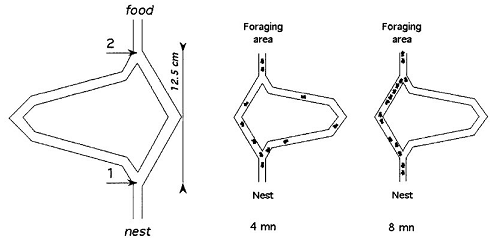
\includegraphics[width=4.0in,height=2.0in]{./pictures/antBridgeExperiment.png}}
	\caption{The shortest path bridge experiment \cite{AntsAndStigmergy}}
	\label{fig:antBridgeExperiment}
\end{figure}

Pheromones used by the ants in \gls{ACO} go through two phases. The first phase is where pheromones a deposited on a particular path by an ant whether there exists previous pheromones or not. The second phase is where pheromones evaporate. Pheromones are not permanent and deteriorate over time\cite{FundamentalSwarm}. By letting pheromones evaporate, ants can ``forget'' previous decisions made by the colony\cite{FundamentalSwarm}. It can be concluded that the more pheromones evaporate the less influence the ants will have on their path selection, therefore promoting exploration\cite{FundamentalSwarm}.

The concept of pheromones and how the \gls{ACO} proceeds in updating the pheromones is a critical concept of \gls{ACO}. Hence, an in-depth discussion on pheromones is provided in subsection \ref{sec:ACOcharacter}.

The \gls{ACO} class of algorithms have a \emph{core requirement} about the problem they are applied to\cite{FundamentalSwarm}. The problem must be able to be modelled as a graph. The reason behind this requirement is that each individual ant in the \gls{ACO} algorithm constructs a path through the graph\cite{FundamentalSwarm}. The path constructed represents a solution.

A path through a graph is made up of a series of links between nodes\cite{AIModernApproach,DataStructuresJava}. A link between two nodes represents a movement from one node to the other\cite{AIModernApproach,DataStructuresJava}. Therefore, a path can be considered as the traversal of the interlinked nodes, from a starting node to some final node\cite{AIModernApproach,DataStructuresJava}. A path differs from another path by the order in which the nodes are interlinked between a start and end node\cite{AIModernApproach,DataStructuresJava}.

 The \gls{ACO} class of algorithms has been applied to a wide range of problems that include single machine scheduling\cite{ACOSingleMachine},weapon target assignment\cite{WeaponTargetACO}, flow shop scheduling\cite{ACOFlowShop} and image thresholding\cite{ACOImageThreshold}. Variants of the standard algorithm have been developed, but all of the algorithms still follow the core structure of the \gls{ACO} algorithm\cite{CompuIntelligenceIntro,FundamentalSwarm}.
The first algorithm developed based on the foraging behaviour of ants is known as the \gls{SACO} and was proposed by Dorigo in 1992 \cite{CompuIntelligenceIntro}. The algorithm provided the basis for how pheromones are used and updated. The \gls{SACO} is an algorithmic implementation of the double bridge experiment.

The first algorithm to improve upon the \gls{SACO} is the \gls{AS} \cite{CompuIntelligenceIntro,AntIntroTrends}. The \gls{AS} included heuristic information into the probability that an ant chooses to move towards a node. The \gls{AS} also added memory to the \gls{AS} by using a tabu list and also incorporated pheromone evaporation. The improvements made enabled the \gls{AS} to better explore the search space and produce better results\cite{CompuIntelligenceIntro,AntIntroTrends}. 

The \gls{AS} algorithm has achieved good success in the problems it has been applied to, but it does have some disadvantages\cite{ImpACOComplex,ACOSurvey}. One of the primary disadvantages of \gls{AS} is that it tends to premature converge on local optima \cite{FundamentalSwarm,ImpACOComplex}. The premature convergence can be attributed to the ants exploiting the high concentration of pheromones on good solution paths too quickly\cite{FundamentalSwarm}. With the ants focusing only on the good solutions less exploration occurs in the search space leading to local optima being produced as the best solution\cite{FundamentalSwarm}.

Subsequently, various algorithms have been developed that improve on the \gls{AS} algorithm. These improved algorithms include the \gls{ACS}, \gls{MMAS}, Ant-Q, fast ant system, AntTabu, \gls{AS}-rank and \gls{ANTS}\cite{CompuIntelligenceIntro,AntIntroTrends}. The discussion in this section is focused on providing an introduction to the general \gls{ACO} algorithm concepts and not to discuss various improvements made by variants of the core algorithm. In the forth-coming sections reference is made to these algorithms and their respective improvements.

The \gls{AS} algorithm is the base algorithm upon which all other \gls{ACO} class algorithms are based upon. Therefore in the forth-coming sections when a reference is made to the \gls{ACO} algorithm, it is directed at the base \gls{AS} algorithm.

In this section the concepts  upon which the core of \gls{ACO} is based upon were briefly introduced. The next section discusses each of these concepts.
\subsection{ACO Characteristics}
\label{sec:ACOcharacter}
In this section characteristics that are important and unique to the \gls{ACO} class of algorithms are discussed. The discussion is focused upon three core characteristics namely pheromone trials, pheromone evaporation, pheromone updates and state transition rules.
\subsubsection{Pheromone Trail}
\label{sec:pheromonetrail}
The pheromone technique used by ants' forms part of the core methodology used by the \gls{ACO} algorithm \cite{AntQAP}. As an ant moves it lays down pheromones to mark the path it is walking.

With the use of pheromones ants are able to communicate the best and shortest link between nodes\cite{AntQAP,AntsAndStigmergy,CompuIntelligenceIntro}. The more ants following a preferred link the more pheromones would be deposited on that specific link. This increases the strength of the pheromones \cite{ImpACOComplex}. The increase in strength of the pheromones on a link would thus let ants more clearly distinguish between links they should and should not take \cite{ImpACOComplex}. Therefore, a pheromone provides positive feedback to the colony\cite{AntQAP,AntsAndStigmergy,CompuIntelligenceIntro}.

Initially, all the ants will choose a random link to a node\cite{AntQAP,AntsAndStigmergy,CompuIntelligenceIntro}. After all the ants have completed their paths, each path is evaluated using a cost function defined by the problem domain\cite{CompuIntelligenceIntro}. The amount of pheromones marking the links contained in a path in the standard \gls{ACO} are related to the cost function\cite{AntQAP,AntsAndStigmergy,CompuIntelligenceIntro}. Therefore, a low cost function value will have a high pheromone dosage and a high cost function value will have a low dosage\cite{CompuIntelligenceIntro}. 

By incorporating the cost of a particular path into the amount of pheromone deposited the colony is able to influence future decisions\cite{CompuIntelligenceIntro}. In terms of minimisation a path with a low cost will have a high pheromone value making the links of path more likely to be selected by future ants\cite{CompuIntelligenceIntro}.

In the iterations following the initial one, the ants will at each node decide based on a probability whether it should move to a particular neighbouring node. The higher the pheromone intensity is at a neighbouring node, the higher the probability that the ant will choose to move towards that node\cite{AntQAP,AntsAndStigmergy,CompuIntelligenceIntro}. The probability with which ants choose links to neighbouring nodes are defined and discussed in the next section.

Due to ants choosing links to node based on a probability, it is still possible for the ant to choose a random link towards another node. Thus the \gls{ACO} algorithms are considered stochastic search procedures due to the ants' ability to choose links randomly when exploring the search space \cite{ACOSurvey,ImpACOComplex}.

The pheromone trail was initially developed with only one colony in mind \cite{CompuIntelligenceIntro}. In research done by Tiwari \emph{et al.}\cite{ACOLargeProblem} pheromones in multiple colonies are considered. The basic principle of how pheromones are used by the ants stays the same, but the meaning of the pheromone changes if an ant of another colony encounters the pheromone trail\cite{AntQAP,AntsAndStigmergy,CompuIntelligenceIntro}. The ant will not follow or even consider the pheromone trail since any pheromone encountered from other colonies repulses the ant\cite{ACOLargeProblem}. Thus pheromones only provide positive feedback if the ant is from the same colony, otherwise the pheromone gives negative feedback, in a way warning the ant to stay away\cite{ACOLargeProblem}. This repulsion strategy promotes exploration among the multiple colonies\cite{ACOLargeProblem}. The probability with which a link towards a particular node is chosen by an ant forms part of the \emph{state transition rules}.

\subsubsection{Pheromone Evaporation}
\label{sec:pheromoneevapuation}
Initially when the pheromone concept was first implemented the ants of the colony rapidly converged on a solution\cite{CompuIntelligenceIntro}. The search space was not adequately explored and the produced solution was of local optima\cite{AntsAndStigmergy}. To combat this premature convergence and force the ants to explore the search space more, the concept of \emph{pheromone evaporation} was introduced\cite{AntIntroTrends,AntSurvey}. 

Real pheromones used by ants to mark a particular link to a node is not permanent and over time the strength of the pheromone deteriorates until it eventually disappears\cite{CompuIntelligenceIntro}. Pheromone deteriorating is known in the literature as pheromone evaporation\cite{CompuIntelligenceIntro}. The pheromone will not completely evaporate as long there are ants traversing the defined link reinforcing the pheromone. The evaporation of pheromones is modelled in the \gls{ACO} by equation \ref{eq:pheromoneevapuration}\cite{AntIntroTrends,AntSurvey}:
\begin{equation}
\label{eq:pheromoneevapuration}
	\tau_{ij}(t) = (1-p)\tau_{ij}(t), p\in [0,1]
\end{equation}
The constant $p$ defines the rate at which the pheromone evaporates. If $p=1$ the pheromone completely evaporates every iteration. With no pheromone on a link towards a node the ants take no knowledge gained from the previous iteration into account and therefore select a link randomly \cite{CompuIntelligenceIntro,AntsAndStigmergy}. Thus, the amount of exploration done by the algorithm can be controlled by the constant $p$ \cite{CompuIntelligenceIntro,AntsAndStigmergy}.

Equation \ref{eq:pheromoneevapuration} was first introduced in the \gls{AS} \cite{CompuIntelligenceIntro,AntSurvey}. Most subsequent algorithms that are a form of the \gls{ACO} class of algorithms also use the concept of pheromone evaporation, but they either use the standard equation or develop their own variant \cite{CompuIntelligenceIntro,AntsAndStigmergy}.

A more aggressive form of pheromone evaporation  is added to the \gls{AS} discussed in the research done by Gambardella \emph{et al.}\cite{AntQAP}. The more aggressive form works beside the already present pheromone evaporation, but this form seeks to add an additional search phase called \emph{diversification}\cite{AntQAP}. The aim of the diversification phase is to lead the algorithm into another direction of the search space\cite{AntQAP}. This is done in an attempt to avoid local minima and stagnation\cite{AntQAP}.

In the ant system developed by Gambardella \emph{et al.} the algorithm continually monitors the current best solution and keeps a history of recent best solutions\cite{AntQAP}. If the algorithm starts to notice that solutions are cycling or that the current best solution has not changed for a certain number of iterations, the algorithm activates the diversification phase\cite{AntQAP}. In this phase the algorithm is forced to re-search the search space to create new solutions, as it cannot rely on previous historical information provided by the pheromone trails\cite{AntQAP}.

\subsubsection{State Transition Rules}
\label{sec:STR}
The intention of this section is not to give an exhaustive survey of different transition rules in the literature. Therefore, only the first transition rule that was developed is discussed, since most of the other rules can be considered derivatives of the first. 

 As discussed previously, the ants select which link to follow towards a node based on a probability. This probability is also known as the \emph{transition probability} and is formulated by equation~\ref{eq:ASprobability}.
\begin{equation}
\label{eq:ASprobability}
p^k_{ij}(t) =
\begin{cases}
	\frac{\tau^{\alpha}_{ij}(t)\eta^{\beta}_{ij}}{\sum_{u \in N^k_i(t)} {\tau^{\alpha}_{iu}(t)\eta^{\beta}_{iu}(t)}}, &\text{if $j \in N^k_i(t)$}\\
	0, &\text{if $j \notin N^k_i(t)$}\\
\end{cases}
\end{equation}
The transition probability is used by individual ants of the \gls{AS} algorithm \cite{AntQAP,FundamentalSwarm}. An ant $k$ uses this equation to decide with what probability it will move from node $i$ to node $j$ \cite{CompuIntelligenceIntro,ACOLargeProblem}. $\tau_{ij}$ is the amount of pheromone on the link between nodes $i$ and $j$ \cite{AntsAndStigmergy,ACOLargeProblem}. Heuristic information is incorporated into the equation through the symbol $\eta_{ij}$, which is the desirability of the link from node $i$ to node $j$ as evaluated by a heuristic function \cite{AntsAndStigmergy,ACOLargeProblem}. 
Each ant starting at a source node moves from one node to another based on the defined transition probability until the ant reaches the final node.

Through the use of parameters $\alpha$ to represent pheromone intensity and $\beta$ to represent heuristic information the algorithm is able to achieve a good balance between exploration and exploitation when $\alpha=\beta$ \cite{ACOLargeProblem,AntQAP}. When $\alpha = 0$ no pheromone is taken into account; hence, any history that the algorithm has on the link between node $i$ and node $j$ is neglected and the algorithm degrades to a stochastic greedy search procedure. If $\beta = 0$ then the algorithm does not take into account the amount of desirability of the link between node $i$ and node $j$ as dictated by the problem-specific heuristic function.

The set $j \in N^k_i(t)$ contains all the valid neighbourhood moves ant $k$ is allowed to make when moving from node $i$ to node $j$. A tabu list is kept by each ant to trim the set of moves already performed previously, and thus cycling is prevented. The interested reader that requires more information about state transition rules is directed to the survey by Engelbrecht\cite{FundamentalSwarm}.
\subsubsection{Pheromone Update}
Pheromones start to evaporate over time, and so the link marked by a pheromone trail becomes less attractive to the ants. Therefore, a path that represents a good solution needs its pheromone trail to be continuously reinforced. Certain rules govern when and by how much pheromones are reinforced.

 Most of the variants that have been developed differ in what pheromone update rules they employ. In the literature pheromone update rules are classified into two groups \cite{CompuIntelligenceIntro}. One group is called the global update rule. The other group is called the iteration-based or local update rule\cite{CompuIntelligenceIntro}. 

The first local pheromone update rule was introduced in the \gls{AS} algorithm \cite{CompuIntelligenceIntro,AntSurvey,AntsAndStigmergy}. The ants would retrace their path after each iteration, depositing pheromones on each link that makes the complete path. The following equation is used to update the pheromone:
\begin{align}
\label{eq:pheromonedeposit}
 \tau_{ij}(t+1) &= \tau_{ij}(t) + \Delta\tau_{ij}(t),\\ 
 \text{where }\Delta\tau_{ij} &= \sum^{n_k}_{k=1}\Delta\tau^k_{ij}(t) \notag
\end{align}
In equation~\ref{eq:pheromonedeposit} $\tau_{ij}(t+1)$ represents the amount of pheromone that will be on the link for the next time step $(t+1)$. $\tau_{ij}$ represents the amount of pheromone currently on the link $(i,j)$. $\Delta\tau_{ij}$ is the actual amount of pheromone that needs to be added to the current pheromone $\tau_{ij}$.

Pheromone update rules that are in the global update group only allow the pheromone trail of the path representing the best-found solution since the first iteration to be updated \cite{CompuIntelligenceIntro}. Thus the global rule favours intensification where the algorithm exploits the global knowledge gained by the ants to find a better solution. By updating a pheromone the concentration of the particular pheromone is reinforced.

\gls{ACS} was the first to use both the global update rule and local update rule together\cite{CompuIntelligenceIntro}. By using both types of rules the algorithm is able to efficiently exploit the history provided by the pheromones\cite{CompuIntelligenceIntro}. The global update rule used by the \gls{ACS} is formulated in the following equation\cite{CompuIntelligenceIntro}:
\begin{align}
\label{eq:pheromoneupdate}
	\tau_{ij}(t + 1) &= (1 - p_1)\tau_{ij}(t) + p_1\Delta\tau_{ij}(t),\\
	\text{where }\Delta\tau_{ij} &= \notag
	\begin{cases}
		\frac{1}{f(x^+(t))} &\text{if $(i,j) \in x+(t)$}\\
		0 &\text{otherwise}
	\end{cases}
\end{align}
The parameter $f(x^+(t))$ represents the best/shortest path found so far by the algorithm\cite{CompuIntelligenceIntro}. $p_1$ is the variable that controls the rate of evaporation. $\Delta\tau_{ij}(t)$ is the amount of pheromone at the current time step $t$ for the link $ij$.

By using the global update rule the algorithm is able to direct the search more, which is to say the algorithm exploits the search space more. Exploitation is achieved since the best path is continually used in the update of the pheromone as can be observed in equation~\ref{eq:pheromoneupdate}\cite{CompuIntelligenceIntro,FundamentalSwarm}.
As can be seen in the following equation, the \gls{ACS} uses a slight variant of the local update rule first used in \gls{AS}\cite{CompuIntelligenceIntro}:
\begin{equation}
	\tau_{ij}(t) = (1 - p_2)\tau_{ij} + p_2\tau_0
\end{equation}
In the above equation $\tau_0$ is a small constant and $p_2 \in [0,1]$ is the constant that defines the rate of evaporation\cite{CompuIntelligenceIntro}. With the local update rule, the algorithm is able to explore more. The path constructed by the individual ant is used to update the pheromone and no information from the best path found in the colony is incorporated, as with equation~\ref{eq:pheromoneupdate}\cite{CompuIntelligenceIntro,FundamentalSwarm}.

The \gls{MMAS} algorithm as discussed also improves on the \gls{AS}. The global update rule used by \gls{AS} has a disadvantage in the sense that the search might concentrate too quickly on a particular good solution (the global best path)\cite{FundamentalSwarm}. \gls{MMAS} address this disadvantage by using the global update rule on an iteration basis\cite{FundamentalSwarm}.

When considering only on a per iteration basis, the best path found by the algorithm can differ from one iteration to the next\cite{FundamentalSwarm}. Therefore the \gls{MMAS} a different path will be updating with the global update rule each iteration\cite{FundamentalSwarm}. Using this approach the algorithm is allowed to explore the search space more\cite{FundamentalSwarm}.

Another shortcoming of the \gls{AS} is that pheromone concentrations can become extremely high leading to less exploration by the algorithm\cite{FundamentalSwarm}. The \gls{MMAS} algorithm addresses this shortcoming by enforcing a maximum and minimum amount of pheromone that can exist on a path\cite{FundamentalSwarm}. By defining a maximum the algorithm is prevents the algorithm from settling on one particular solution i.e. stagnation\cite{FundamentalSwarm}. On the other hand, defining a minimum on all possible links between nodes ensures that links will be continuously considered for possible inclusion into a solution\cite{FundamentalSwarm}. In addition to providing boundaries for the pheromones \gls{MMAS} also uses a smoothing strategy to even out the difference between high and low pheromones\cite{FundamentalSwarm}.

\subsection{Flow of the Algorithm}
In this section the process the \gls{AS} algorithm uses to explore the search space is described. Algorithm~\ref{alg:ACO} is used as a reference point.
\begin{algorithm}[H]
\caption{Ant System Algorithm~\cite{CompuIntelligenceIntro}}
\label{alg:ACO}
	\begin{algorithmic}[1]
	\State$\text{Initialize $\tau_{ij}$ with small starting values}$
	\State$t \leftarrow 0$
	\State$\text{Place $n_k$ ants on starting node}$
	\While{stopping condition not reached}
		\For{each ant $k \leftarrow 0$ to  number of ants $n_k$}
			\State$p^k(t) \leftarrow \text{Initialize path } p^k \text{for time step } t$
			\Repeat
				\State$\text{Select next node based on probability equation~\ref{eq:ASprobability}}$
				\State$\text{Add link (i,j) to path } p^k(t)$
			\Until{Final node reached}
			\State$x^k(t) \leftarrow \text{Remove loops from path }p^k(t)$
			\State$\text{Calculate length of path $f(p^k(t)$})$
		\EndFor
		\For{each link $(i,j)$ in graph}
			\State$\tau_{ij} = \text{Reduce pheromone of link $(i,j)$ with equation~\ref{eq:pheromoneevapuration}}$
		\EndFor
		\For{each ant $k = 0$ to  number of ants $n_k$}
			\For{each link $(i,j)$ in $p^k(t)$}
				\State$\triangle \tau_{ij} = \frac{1}{f(p^k(t))}$
				\State$\text{Update the pheromone $\tau_{ij}$ with equation~\ref{eq:pheromoneupdate}}$
			\EndFor
		\EndFor
		\State$t \leftarrow t + 1$
	\EndWhile\\
	\Return $\text{path $x^k(t)$ with the smallest $f(x^k(t))$ as the solution}$
	\end{algorithmic}
\end{algorithm}

The \gls{ACO} algorithm initialises by creating a set population of ants and placing them on random starting nodes as well as initialising the pheromones to starting values as can be observed from algorithm~\ref{alg:ACO}, lines 1 -- 3. The main purpose of the ant is to explore the search space and to ultimately produce a solution that might be optimal. The ant explores the search space by performing a series of moves from one node to another. Each move is a link that is added to the path. This process can be seen in lines 5 -- 10.

The ant selects which node to move to next based on a probability. The probability is calculated taking into account the amount of pheromone that is on the current link representing the movement from the current node to the next node\cite{CompuIntelligenceIntro,FundamentalSwarm}. This decision process can be seen to occur in line 8.

As the ant moves it records each link between the nodes it traverses until it reaches the final node. All the links the ant has traversed represent a path taken through the search space\cite{CompuIntelligenceIntro,FundamentalSwarm}. Thus, as the ant is moving it is actively building an optimal solution.

Before the ant deposits pheromone on the links it traversed to construct its solution, the pheromones first need to be decayed. This is why in lines 14 -- 16, the algorithm traverses all links that contain pheromones and reduces the amount of pheromones by applying equation~\ref{eq:pheromoneevapuration}.

Once an ant has constructed a path and the pheromone evaporation has occurred, the ant is ready to inform the rest of the ants of what movements it made to construct its solution. The ant needs to share this movement information in order for the rest of the colony to know which movements worked well and which did not. The ant therefore needs to signal the other ants, which is accomplished with pheromones. Therefore, in the next phase of the algorithm, pheromones are deposited on all the links that make up the path the particular ant constructed. In the algorithm pheromones are deposited on lines 17 -- 22 in algorithm~\ref{alg:ACO}.

After all the ants have deposited pheromones on all the links represented by each individual ant's constructed solution, the algorithm is ready to continue to its next iteration. This process occurs until some defined stopping criterion occurs.

\subsection{ACO on the \gls{FAP}}
ACO has been applied to a wide number of problems like weapon targeting\cite{WeaponTargetACO}, flow shop scheduling\cite{ACOFlowShop} and quadratic assignment\cite{AntQAP} where it has achieved good results. As discussed in chapter~\ref{chpt:fap}, the \gls{FAP} can be modelled as a graph and therefore the \gls{ACO} has also been applied to it\cite{ACOvsEA}.

When using the \gls{ACO} algorithm on the \gls{FAP} the ants need to construct a path that represents a frequency plan and has low interference. With the \gls{ACO}, a node is a cell that has a unique set of channels assigned to it. Thus the same cell may exist in the search space, but will have a different set of channels assigned to it, and will therefore represent an entirely different node to the \gls{ACO}.

As an ant moves in the frequency planning domain, it is actually moving between two cells that are said to interfere. The interference between two cells occurs as a consequence of the channels that have been assigned to them. 

As an ant completes a movement from one cell to another, i.e it assigns channels to the cell, it measures the interference that occurs due to the assignment.  The measured interference information is incorporated into the pheromone, which the ant will deposit on the link between the two cells.

An optimal frequency plan would therefore be a path through all the interfering cells marked with a high dosage of pheromone. As discussed in the previous sections, the pheromone indicates the desirability of a particular path. In the \gls{FAP}, a desirable path would be one where interference is low; thus a path with a high dosage of pheromones would be the frequency plan with the lowest interference found by the algorithm.
When analysing the basic \gls{ACO} algorithm~\ref{alg:ACO} one can identify the following possible disadvantages if the algorithm were applied to the \gls{FAP}:
\paragraph{Memory Usage}
--- The algorithm requires a fair amount of memory. The memory is used to keep track of each permutation of a particular cell and its allocated frequencies until the pheromone that links to the cell has decayed enough to be discarded. As an ant moves from one cell to another, it might not select the previous cell (due to probability) to move to, but rather generates an entirely new cell to move towards. This newly generated cell would then be linked to the previous cell, and therefore the algorithm needs to keep track of the pheromone on that link until it has completely been decayed away. The algorithm needs to keep track of these pheromones on the links even if the new link to the generated cell is not even close to optimal and has very high interference.
\paragraph{Building a solution}
--- The \gls{ACO} \emph{builds} an optimal solution. Therefore, early decisions made by the ants still influence the plan later for better or for worse. A good decision might seem to be good early on, but later the algorithm might be better off with a slightly worse decision. In the \gls{FAP}, a cell can have multiple interfering cells, but a particular ant only knows about one link between two cells and not about the other interfering cells. Thus an ant will find the optimal path on the first interfering link between two cells, in other words it will optimise the channels allocated to these cells so that interference is low. The first interfering link is now optimised, and subsequent ants will reinforce this channel allocation since the interference is low. When the ants later reach the other cells that also interfere with the first cell that has been optimised, they will have difficulty changing the assignments that have already been made, since the pheromone representing that assignment is too strong to disregard.

The above disadvantages have only been identified by critically evaluating the algorithm as a possible point of interest to produce an optimal solution for the \gls{FAP} for this dissertation. Even with these disadvantages the \gls{ACO} has achieved success in producing high quality optimal solutions for the \gls{FAP}.

In research conducted by Luna \emph{et al.}\cite{ACOvsEA} an \gls{ACO} algorithm was applied to a custom cellular network instance. This network instance had 711 sectors with 2 612 transceivers, which needed to be assigned frequencies. For their particular network, only 18 channels were available for assignment. The channels started at 134 and ended at 151\cite{ACOvsEA}.
The authors presented two versions of the algorithm. The first version used no heuristic information (henceforth referred to as \gls{ACO}*) and the other version used heuristic information to update the pheromone laid done by the artificial ants\cite{ACOvsEA}.

With regard to the heuristic updating of the pheromone trails, the authors opted to increase the pheromone by some magnitude\cite{ACOvsEA}. This magnitude was hand tuned to be 100. The heuristic only increases a certain path's pheromone if the frequencies assigned to the transceivers represented by this path differ enough so as to not cause significant interference\cite{ACOvsEA}. Thus, the heuristic aims to amplify good choices made previously by the algorithm for the next iteration of the algorithm.

In table~\ref{tab:ACO} the results obtained by Lune \emph{et al.} \cite{ACOvsEA} is presented. By evaluating the results obtained, one can clearly see that the \gls{ACO} version that incorporates heuristic information to reinforce pheromone trails outperforms the version that does not \cite{ACOvsEA}. 
\begin{table}[H]
\centering
	\begin{tabular}{| c | c | c |}
	\hline
	Time limit & \gls{ACO}* & \gls{ACO} \\ \hline
	120s & 104719.72 & 91140.04 \\ \hline
	600s & 103752.12 & 89703.44 \\ \hline
	1 800s & 103781.86 & 88345.94 \\ \hline
	\end{tabular}
\caption{ACO and \gls{ACO}* on custom GSM \gls{FAP} benchmark\cite{ACOvsEA}}
\label{tab:ACO}
\end{table}
The values depicted in the table represent the amount of interference that will result if the plan is used in the network\cite{ACOvsEA}.The values depicted in the table represent the amount of interference that will result if the plan is used in the network\cite{ACOvsEA}. The following section discusses the Artificial Bee Algorithm.
\section{Artificial Bee Colony (ABC) Algorithm}
\label{sec:BEE}

\subsection{Introduction}
The \gls{ABC} algorithm is the most recently presented algorithm in the literature discussed in this chapter\cite{ABCCompareStudy,ABCLeafConstrained,ABCNumericalOptimization}. The algorithm was first proposed by Karaboga in 2005 who wanted to mimic the foraging behaviour exhibited by bees \cite{ABCCompareStudy,ABCLeafConstrained,ABCNumericalOptimization}. Like ants, bees need to gather food to support the colony. To understand how the \gls{ABC} algorithm tries to mimic the foraging behaviour of bees, this behaviour of real bees needs to be described first\cite{ABCCompareStudy}. 

In a bee colony there are numerous bees, each with a specific role that dictates what actions a bee can perform. There are bees that protect the queen, maintain the colony, scout for resources and gather food, i.e. the worker bees. The most important bees for foraging are those that scout and gather food\cite{ABCCompareStudy}. 

The scout bees are sent out and as their role implies, they are responsible for exploring the surroundings of the hive to find suitable food sources\cite{ABCCompareStudy}. If a scout bee has found a food source it needs to return to the colony to share the information with the worker bees\cite{ABCCompareStudy}. When the bee enters the colony it needs to communicate to the other bees by using some form of stigmergy (see section~\ref{sec:stigmergy})\cite{ABCCompareStudy}.

The scout bee accomplishes this communication by performing a dance known as the \emph{waggle dance} in the colony for all the bees to see\cite{ABCCompareStudy}. This is not a dance as in the traditional sense, since through certain movements the bee is able to communicate a variety of characteristics about the food source including\cite{ABCCompareStudy}:
\begin{itemize}
\item How far the food source is from the colony
\item Quality of the food source
\item Path towards the food source
\end{itemize}

It can be concluded that foraging bees use \emph{sematectonic} stigmergy (discussed in section~\ref{sec:stigmergy}). This is deduced from the dance, which is a physical form of communication.

The dance is observed by \emph{onlooker} worker bees \cite{ABCCompareStudy,ABCImageEnhancement}. These onlooker bees are initially \emph{unemployed} in the colony \cite{ABCCompareStudy,ABCImageEnhancement}. Once the information of the scout has been transferred to the onlooker bees, the onlooker bees become \emph{employed} bees\cite{ABCCompareStudy,ABCImageEnhancement}. They become employed bees when they operate on a particular food source to gather food\cite{ABCCompareStudy,ABCImageEnhancement}. Thus it is the job of the worker bees to \emph{exploit} the information provided by the \emph{exploration} done by the scout bees \cite{ABCCompareStudy,ABCNumericalOptimization}. 

Worker bees gather food from the designated food source, until the food source reaches a certain quantity with regard to nectar content \cite{ABCCompareStudy,ABCNumericalOptimization}. Each time the bee returns to the colony it evaluates the current food source versus other food sources discovered \cite{ABCCompareStudy,ABCNumericalOptimization}. If a better food source is found, the bee abandons the previous source and starts gathering food from the new source \cite{ABCCompareStudy,ABCNumericalOptimization}. On the other hand, if the food source has been exhausted, meaning there is no more nectar content to gather, the bee returns to the colony and becomes ``unemployed'' \cite{ABCCompareStudy,ABCNumericalOptimization}.

In the \gls{ABC} algorithm, possible solutions are considered to be food sources\cite{ABCCompareStudy,ABCNumericalOptimization}. Each food source has an employed bee associated with it. Onlooker bees either wait for new food sources to be communicated to them or become employed bees by moving to another, more attractive food source \cite{ABCCompareStudy,ABCNumericalOptimization}. 

A food source might be more attractive to a bee because its defined nectar content is more than that of the current food source the bee is operating on\cite{ABCCompareStudy,ABCNumericalOptimization}. The nectar content of a food source can be considered to be the fitness, which is determined using the fitness function of the specific problem domain\cite{ABCCompareStudy,ABCNumericalOptimization}.

As with real honeybees, a \emph{waggle dance} is performed to all the onlooker bees by employed bees that provide information on the nectar amount (fitness value) that they represent \cite{ABCReconfigDistro,ABCCompareStudy,ABCImageEnhancement}. The onlooker bees choose food sources depending on the nectar amount \cite{ABCReconfigDistro,ABCCompareStudy,ABCImageEnhancement}; therefore as the nectar amount of a food source increases, the probability that more onlooker bees will choose the source increases \cite{ABCReconfigDistro,ABCCompareStudy,ABCImageEnhancement}. How and what affects the probability is discussed in the next subsection.

Bees can transition to different roles depending on their situation \cite{ABCCompareStudy,ABCNumericalOptimization}. An onlooker bee becomes employed when assigned to a food source and an employed bee can become a scout if its initial food source becomes exhausted \cite{ABCImageEnhancement,ABCCompareStudy,ABCReconfigDistro}. Note that not all employed bees of a food source become scouts; only the first employed bee of a food source transitions to a scout \cite{ABCImageEnhancement,ABCCompareStudy,ABCReconfigDistro}. Scout bees are sent to randomly generated food sources \cite{ABCImageEnhancement,ABCCompareStudy,ABCReconfigDistro}. 

The more onlooker bees a food source attracts, the more the neighbourhood will be explored since the onlooker bees move to the food source and choose an immediate neighbouring food source to be employed upon \cite{ABCCompareStudy,ABCNumericalOptimization}. Thus, this can be considered exploitation and the algorithm is therefore performing a local search\cite{ABCCompareStudy,ABCReconfigDistro,ABCNumericalOptimization}. Finally, the number of onlooker bees a food source has also indicates its desirability. A very good solution will have the majority of onlooker bees choosing it and searching for nearby better food sources \cite{ABCCompareStudy,ABCReconfigDistro,ABCNumericalOptimization}. More bees are lured towards a particular food source due to the high nectar amount that has been communicated to them by other employed bees\cite{ABCCompareStudy,ABCReconfigDistro,ABCNumericalOptimization}.

When a food source is abandoned, the previous bee that occupied the food source transitions to a scout bee \cite{ABCCompareStudy,ABCNumericalOptimization}. The scout bee is responsible for replacing the abandoned food source by finding a new one, and a new food source is generated and communicated back to the colony\cite{ABCCompareStudy,ABCImageEnhancement,ABCNumericalOptimization}. The generation of food sources is discussed in the next subsection.

Karaboga was not the first to base an algorithm on the above foraging behaviour. Other bee foraging inspired algorithms have been developed such as the BeeHive algorithm, \gls{BCO} and \gls{BSO} \cite{BCO,HybridABCClustering,ABCNumericalOptimization}. 

The BeeHive algorithm is based on the dance communication used inside the colony of bees. In \gls{BCO} solutions are randomly generated and assigned to bees\cite{HybridABCClustering,ABCNumericalOptimization}. Finally, \gls{BSO} solutions are iteratively constructed by forager (worker) bees and the best solution is communicated to the rest of the colony by performing a dance\cite{HybridABCClustering,ABCNumericalOptimization}.

Another bee algorithm is the \gls{VBA}, which like the previous algorithms, is also based on the foraging behaviour of bees, but it differs in that it is not designed for combinatorial problems \cite{ABCNumericalOptimization}. Instead the \gls{VBA} is a variant of the standard \gls{ABC} algorithm, which is designed for numerical function optimisation \cite{ABCNumericalOptimization}. In \gls{VBA} bees move around in the search space communicating to each other any target nectar food sources that are found\cite{ABCNumericalOptimization}. Good food sources are function evaluations of particular coordinates in the numerical search space, which produce low function evaluation values in the case of minimisation\cite{ABCNumericalOptimization}.

Karaboga developed the \gls{ABC} algorithm based on the previous research done on bee colony optimisation and the above algorithms. The \gls{ABC} algorithm is designed to be a multivariable optimisation algorithm and has to date been applied to the job scheduling problem, clustering \cite{HybridABCClustering}, neural network training and reconfiguration of distribution networks \cite{ABCReconfigDistro}. Due to the nature of the algorithm being similar to that of the \gls{ACO}, the \gls{ABC} algorithm will most likely also be applied to a whole host of other of problems.

\subsection{ABC Algorithm Characteristics}
Various characteristics of the \gls{ABC} algorithm define the algorithm and make it unique. The first characteristic is how food sources are handled in the algorithm. The second is how information is communicated to the colony.
\subsubsection{Food Sources}
\label{sec:foodsources}
As discussed previously, food sources represent solutions to the problem the \gls{ABC} algorithm is being applied to. When the algorithm starts, there are no defined food sources for the bees to evaluate and report on, and therefore initially a finite number of food sources are randomly generated\cite{ABCCompareStudy,ABCFusionGrid}. Since each food source needs an employed bee to evaluate the nectar amount of the source, the parameter that defines the number of food sources also defines the number of employed bees\cite{ABCCompareStudy,ABCLeafConstrained}.

Employed bees evaluate these food sources by determining their nectar amount\cite{ABCCompareStudy,ABCLeafConstrained}. The nectar amount is directly related to the fitness value calculated using a domain specific cost function\cite{ABCCompareStudy,ABCReconfigDistro}. After the amount is determined the employed bee advertises the food source to the colony by performing the waggle dance.

Onlooker bees witness a number of dances from a variety of employed bees\cite{ABCFusionGrid,BeeJobShop}. They therefore need to select a food source that is the most attractive while maintaining some diversity in the pool of solutions. Thus, an onlooker bee selects a food source based on a probability function which is formulated in equation \ref{eq:beeProbability}\cite{ABCCompareStudy}:
\begin{equation}
\label{eq:beeProbability}
p_i = \frac{{fit}_i}{\sum^{SN}_{n=1}{fit}_n}
\end{equation}

The parameter $p_i$ is the $i$th food source under consideration by the onlooker bee. The ${fit}_i$ parameter represents the value of the cost function and is directly related to the nectar amount of food source $i$. The parameter SN is the maximum amount of food source and hence the maximum employed onlooker bees \cite{ABCCompareStudy}.

In algorithm~\ref{alg:ABC} the waggle dance can be seen being applied in line 11 where the probability of all the employed bee' solutions are calculated using equation~\ref{eq:beeProbability}. From lines 12 -- 16 the onlooker bees evaluate the solutions of the employed bees based on the probability $p_i$ that was calculated. $P_i$ can be seen as the rating of the waggle dance that was performed by the employed bee.

\subsubsection{Employed and Onlooker Bees}
\label{sec:employonlookerbees}
As previously outlined, when recruited onlooker bees reach the advertised food source that is stored in memory, they do not occupy the same food source\cite{ABCCompareStudy,ABCNumericalOptimization}. Instead the bees explore the immediate neighbourhood of the food source that was communicated to them\cite{BeeJobShop,ABCFusionGrid,ABCReconfigDistro}. They seek to find a food source that improves on the previous one\cite{BeeJobShop,ABCNumericalOptimization}. Equation \ref{eq:beeGenerate} is used by the bees to generate new food sources in the neighbourhood of food source $x_i$\cite{ABCCompareStudy,ABCFusionGrid}.
\begin{equation}
\label{eq:beeGenerate}
v_{ij} = x_{ij} + \phi_{ij}(x_{ij} - x_{kj})
\end{equation}
The subscripts $k \in \{1,2,\dots,SN\}$ and $j \in \{1,2,\dots,D\}$ are indices which are randomly chosen. $D$ is the maximum dimensionality of the vector a solution represents. The index $k$ has a constraint tied to it -- whatever value is randomly assigned to $k$ \emph{must} differ from the value $i$. The position of the new food source in the neighbourhood of $x_{ij}$ is controlled by the $\phi_{ij}$ parameter, which is a bounded random value between $[-1,1]$. 

From equation \ref{eq:beeGenerate} it can be concluded that the randomness of the food source position decreases as the difference between $x_{ij} - x_{kj}$ decreases. Thus, as the algorithm moves closer to an optimal solution the finer grained the search process of the algorithm becomes\cite{ABCCompareStudy,ABCNumericalOptimization,ABCImageEnhancement}.

After a new solution $v_i$ is produced, the bee takes the new and old solutions from memory to compare their respective nectar contents. If the new solution is found to have higher quality nectar, the bee replaces the old solution in memory with the new solution\cite{ABCCompareStudy,ABCReconfigDistro}. Otherwise, the bee abandons the new solution and keeps the old solution in memory\cite{ABCCompareStudy,ABCNumericalOptimization}. Thus, the bee seeks to always move towards a better solution and therefore uses a greedy selection process\cite{ABCLeafConstrained,ABCReconfigDistro}.

One of the problems with the above approach is that little information about the food source is used in generating a neighbouring food source. Research by Singh \cite{ABCLeafConstrained} proposed a slight variation to generating food source neighbours by using more global information. The author adds a constraint to the algorithm that all neighbouring solutions generated by \emph{employed} bees must be unique. 

When an employed bee generates a neighbour and an identical solution already exists in the system, a \emph{collision} is said to have occurred. A collision is solved by letting the employed bee transition to a scout bee so that a completely random solution can be generated \cite{ABCLeafConstrained}. Scout and onlooker bee generated solutions are not checked if they collide with other solutions in the system since the aim for them is exploring and not exploiting as with employed bees\cite{BeeJobShop,ABCCompareStudy}. 
\subsubsection{Scout Bee}
The artificial bees are modelled on the behaviour of real bees. Thus an employed bee can also abandon certain food sources when it has outlived its usefulness. Abandonment of a food source can occur for the following reasons\cite{BeeJobShop,ABCNumericalOptimization,ABCImageEnhancement}:
\begin{itemize}
\item The employed bee has reached the maximum allowed cycles to improve the nectar amount. The maximum cycles spent on a food source allow the algorithm to avoid local optima\cite{ABCCompareStudy,ABCNumericalOptimization,ABCImageEnhancement}.
\item The bee cannot improve the search represented by the food source any further\cite{ABCCompareStudy,ABCNumericalOptimization,ABCImageEnhancement}.
\end{itemize}
When a food source in the algorithm is abandoned, it needs to be replaced by a new food source\cite{BeeJobShop,ABCCompareStudy,ABCImageEnhancement}. Note that a food source is not abandoned when it represents the globally best-found solution. An employed bee transitions to a new role when it abandons a food source from an employed bee to a scout bee\cite{ABCCompareStudy,ABCNumericalOptimization,ABCImageEnhancement}. 

It is the responsibility of the scout bee to replace the abandoned food source with a new randomly generated one\cite{BeeJobShop,ABCCompareStudy,ABCImageEnhancement}. The scout bee uses equation \ref{eq:scoutGenerate} to produce a new food source that will replace food source $x_i$.
\begin{equation}
\label{eq:scoutGenerate}
x_{ij} = x_{yj} + rand[0,1](x_{zj} - x_{yj})
\end{equation}

The subscript $y$ represents the minimum value of $i$ and the subscript $z$ represents the maximum value of $i$.
In research done by G\'{o}mez-Iglesias \emph{et al.} \cite{ABCFusionGrid} an extension is made to the scout bees. The scout bee individuals are divided into two types of bees, namely \emph{rovers} and \emph{cubs'} bees\cite{ABCFusionGrid}.
\begin{itemize}
\item{Rover bees} are similar to traditional scout bees and hence use diversification strategies to explore the search space. 
\item {Cub bees} explore the search space relative to a good solution found by a rover by randomly changing configuration parameters. 
\end{itemize}
By using two different scout bees a good balance is achieved when searching the search space in the beginning where diversity is preferred and late in the algorithm where intensification is preferred \cite{ABCFusionGrid}.

The following subsection describes the general flow of the \gls{ABC} algorithm. The discussion of the algorithm aids in the understanding of how the algorithm searches a particular problem space. 
\subsection{Flow of the Algorithm}
Most of the concepts that are used in the \gls{ABC} algorithm have been explained. The general search process of the algorithm will now be discussed using algorithm~\ref{alg:ABC} as a reference point.
\begin{algorithm}[H]
\caption{Basic Artificial Bee Colony Algorithm\cite{ABCCompareStudy}}
\label{alg:ABC}
	\begin{algorithmic}[1]
		\State$b_n \leftarrow \text{Initialize bees}$
		\State$s_n \leftarrow \text{Initialize starting solutions}$
		\State$\text{Evaluate starting solutions with fitness function $f(s_n)$}$
		\State$t \leftarrow 0$
		\While{stopping criteria not met}
			\For{each employed bee $eb_i = 0$ to max bees $b_n$}
				\State$\hat{v_i} \leftarrow \text{Generate new solution with equation~\ref{eq:beeGenerate}}$
				\State$\text{Evaluate with fitness function $f(\hat{v_i})$}$
				\State Apply greedy selection between $\hat{v_i}$ and the current solution $\hat{s_i}$ of bee $eb_i$
			\EndFor
    \State$\text{Calculate probability $p_i$ for solutions $\hat{s_i}$ in $\hat{s_n}$ using equation~\ref{eq:beeProbability}}$
			\For{each onlooker bee $ob_i \leftarrow 0$ to max bees $b_n$}
				\State$\hat{x_i} \leftarrow \text{Select solution $\hat{s_i}$ based on $p_i$} $
				\State$\hat{v_i} \leftarrow \text{Generate new solution with $\hat{x_i}$ and $p_i$}$
				\State$\text{Evaluate $\hat{v_i}$ with fitness function $f(\hat{v_i})$}$
				\State$\text{Apply greedy selection between $\hat{v_i}$ and bee $ob_i$ current solution}$
			\EndFor
			\If{there is an abandoned solution for a scout bee}
				\State Replace with solution generated with equation~\ref{eq:scoutGenerate}
			\EndIf
			\State$t \leftarrow t + 1$
		\EndWhile
	\end{algorithmic}
\end{algorithm}
The algorithm starts off by generating a set number of possible solutions. The number of solutions is equal to the number of employed bees. Each starting solution is evaluated using a fitness function. The operations that perform these functions can be observed to occur from lines 1 -- 3.

At first each bee is assigned to one of the initial generated solutions (food sources). Hence the bees start off as employed bees and each bee has in its memory a particular possible solution with an associated nectar amount. The algorithm can now be considered to be initialised, and therefore the algorithm enters the next phase, which is where the actual optimisation and search procedure occurs. This phase stretches from lines 5 -- 22.

From lines 6 -- 10, each employed bee modifies its particular solution based on local information, which is also referred to as visual information in the literature. The modified solution is then tested to determine its nectar amount, i.e the fitness of the generated solution is calculated. The employed bee then compares the newly generated nectar amount with the nectar amount of the search in the bee's memory. If the newly generated solution has a better nectar amount, the bee replaces the current solution in its memory with the newly generated solution.

After all the employed bees have determined whether to keep the newly generated solution or keep the one in memory, they then need to communicate to the rest of the bee hive the nectar amount of the food sources that they occupy. This phase is where the waggle dance occurs and can be observed in algorithm~\ref{alg:ABC} from lines 12 -- 17.

Each onlooker bee then selects which food source it will move towards based on a probability. The probability takes into account the nectar amount that was communicated through the waggle dance by a particular employed bee. The probability is calculated using equation~\ref{eq:beeProbability} which is discussed in section~\ref{sec:foodsources}.

Once an onlooker bee has selected a food source based on the calculated probability, it then starts to search the immediate neighbourhood of the selected food source for other food sources. The neighbouring food sources are generated using equation~\ref{eq:beeGenerate} which is discussed in section~\ref{sec:employonlookerbees}. This procedure of generating neighbouring food sources by an onlooker bee can be observed in line 14 in algorithm~\ref{alg:ABC}.

The onlooker bee then applies the same procedure as an employed bee with regard to determining if the newly generated food source should be remembered or discarded. The bee does this by evaluating each generated neighbouring food source to determine its nectar amount, which is then compared to the nectar amount of the food source in the bee's memory.

In the last phase of the algorithm (before the next iteration starts) the algorithm determines which food sources have been abandoned by the bees. A food source in the algorithm can be abandoned if, for a certain number of iterations the food source has not improved, meaning its nectar content has not increased. When a food source is abandoned the employed bee that occupied the particular food source transitions to a scout bee.

A scout bee aims to replace the abandoned food source with a new food source. In algorithm~\ref{alg:ABC} this occurs in lines 18 -- 22. The scout bee uses equation~\ref{eq:scoutGenerate} to generate a new food source. It then transitions to an employed bee and occupies the newly generated solution. The newly generated food source will now also be evaluated to determine its nectar amount as the rest of the employed bees do at the start of the next iteration.


\subsection{ABC algorithm on the \gls{FAP}}
The \gls{ABC} algorithm and all its variants are relatively new. To date it has only been applied to a select few problems such as the traveling salesman problem.

As yet, no research has been done to apply the \gls{ABC} algorithm to the \gls{FAP}. The following critique is based on a theoretical implementation of the \gls{ABC} algorithm on the \gls{FAP}. Based on this evaluation the following obstacles can be identified if one were to apply the algorithm to the \gls{FAP}:
\paragraph{Food source representation}
--- Each food source can either represent a frequency plan or it can be a particular cell and a collective of food sources represents a frequency plan. If each food source is a frequency plan the algorithm will require a fair amount of memory, since as onlooker bees select it, they will start searching for neighbouring solutions. These neighbouring solutions are \emph{also} frequency plans. However, if each food source were a cell, this would require less memory. The problem with the latter approach is that the bees would then single out one cell as the optimum, since they do not know that all food sources collectively represent a plan and each cell is actually unique.
\paragraph{Scout bee generation}
--- When a food source is abandoned a scout bee needs to generate a new food source to take its place. In particular with the \gls{FAP}, the newly generated solution cannot be completely random. The scout bee needs to incorporate knowledge already gained by the colony operating on different food sources, otherwise a completely random solution might not be even nearly lucrative enough for the rest of the bee colony to consider if it contains no knowledge gained by the algorithm.
\paragraph{Knowledge sharing}
--- As a food source becomes more popular due to its high nectar amount, more onlooker bees will select it. By selecting the food source the onlooker be will then proceed to search in its neighbourhood for better solutions. Therefore the bees are disregarding previously gained knowledge while searching for neighbouring sources on \emph{other} food sources. If a food source represents a complete frequency plan, a previous food source a bee operated on might have had one or more cells that were assigned to their optimal frequencies. Due to the larger majority of the cells not being optimised, these \emph{good} cells are overshadowed. Thus due to the \emph{bad} cells overshadowing the good cells, the food source nectar amount becomes lower. As a consequence of the low nectar amount by the food source the bees abandon the food source and those optimal cells are lost.

The above obstacles present real relevant challenges that would require new techniques to be developed. As the algorithm has not been applied to a wide variety of problems and taking into account the above obstacles, it is difficult to gauge if the \gls{ABC} is well suited to be applied. The algorithm first needs to be applied to a wider set of problems. Once the algorithm has matured in the research behind it the algorithm can be revisited and applied to the \gls{FAP}.

In this section the various obstacles one would encounter when applying the \gls{ABC} class of algorithms to the \gls{FAP} were identified. This concludes the discussion on the \gls{ABC} algorithm. The next section deals with the particle swarm optimisation algorithm.
\section{Particle Swarm Optimisation (PSO)}

\label{sec:PSO}
\subsection{Introduction}
\label{sec:psointro}
PSO is population-based stochastic search technique that was developed by Kennedy and Ebenhart in 1995 \cite{PSOGABreeding}. The basic model of the algorithm is based on simulations done to recreate the natural behaviour of a flock of birds \cite{PSOSoftTesting}.

In the early stages of the particle swarm development, simulations were developed to closely model the stigmergy (see page \pageref{sec:stigmergy} for a discussion on stigmergy) exhibited when a flock of birds cohesively move as one and are able to suddenly change direction in a unpredictable, graceful manner, only to regroup as one observed entity \cite{PSOHybridJobShop}. 

As the ``leading'' bird of the flock changes its movements the information is shared with all birds in the immediate vicinity of the leading bird. As the information is shared locally among birds, each bird modifies his own movement to that of the leading bird's movement\cite{PSOHybridJobShop}. 

Because birds obtain information by observing their neighbouring birds, the stigmergy can be deemed to be of a physical nature; therefore the particular stigmergy used by birds is sematectonic stigmergy (see page \pageref{def:sematectonic}).

The simulations based on this behaviour of the flock allowed researchers to discover the underlying patterns that governed the way birds are able to share information about the general movement of the flock. Based on these patterns and simulations, the particle swarm algorithm emerged into an optimisation algorithm \cite{CompuIntelligenceIntro}.

In the algorithm a particle is an individual\cite{FundamentalSwarm}. A group of particles, referred to in the literature as a swarm,  are moved through the search space of the problem the algorithm is being applied to\cite{FundamentalSwarm}. Each particle changes its movement based on information shared with it by neighbouring particles in the swarm \cite{FundamentalSwarm,CompuIntelligenceIntro}. 

As information is shared among particles, the success of one particle ripples through the rest of the swarm and each particle is able to utilise shared information that leads to success of another particle. Thus, each particle's own personal experience and knowledge of the search space has an effect on its neighbouring particles \cite{FundamentalSwarm,CompuIntelligenceIntro}.

Two variants of the initial \gls{PSO} algorithm were developed namely the global \gls{PSO} and local \gls{PSO}. The only difference between the two algorithms is how they go about sharing information with the rest of the swarm. The sharing models of these two algorithms along with other sharing models are discussed in the \gls{PSO} characteristics subsection \cite{SOSwarm}.

In the swarm, each particle is a potential solution that is represented by a D-dimensional vector \cite{PSOHybridJobShop,PSOSelfHierarch}. As a particle moves through the search space, it continually evaluates its current position and adjusts it accordingly to move in the general direction of its own personal best position and the position of the best particle in its neighbourhood. 

A particle evaluates its current position by using a heuristic function, or in more evolutionary algorithm terms, a fitness function. The fitness value indicates to the particle how far it is from an optimal position\cite{CompuIntelligenceIntro}. 

As a particle moves through the search space it keeps a memory of the personal best position it has achieved since the start of the algorithm. In the literature and in the algorithm this personal best position is referred to as \emph{pbest} \cite{SOSwarm}.

Most of the research done on \gls{PSO} has focused on the convergence of the algorithm as well as improving the diversity \cite{FundamentalSwarm}. Some of these improvements and modifications are discussed in the subsection on \gls{PSO} characteristics.

\subsection{PSO Characteristics}
\label{sec:psocharacteristics}
The defining characteristics of the \gls{PSO} algorithm are discussed in this section. The characteristics include \emph{neighbourhood topology}, \emph{the particle swarm}, \emph{movement of particles} and \emph{keeping particle velocities in check}.
\subsubsection{The Particle Swarm}
The initialising of particles in a swarm are the same as used by traditional population-based evolutionary algorithm to initialise their respective populations \cite{FixedFAPPSO}.  At the start of the algorithm the swarm is initialised by randomly generating possible solutions that will represent the position of particles\cite{CompuIntelligenceIntro}. 

The \gls{PSO} algorithm in some aspects resembles evolutionary algorithms like the genetic algorithm since it also has a population that operates in the problem space in search of an optimal solution. By utilising good mutation operators the \gls{GA} is able to insert new genetic material into the population. At least in the initial search phase of the GA, this increases diversity\cite{CompuIntelligenceIntro}. The \gls{PSO} does not continually generate new solutions to be reinserted into the swarm to increase diversity \cite{PSOHybridUnitCommit}. Thus the swarm size needs to be adjusted to get an optimal representation of the search space because as particles move in the swarm, the diversity among particles decreases rapidly as information is shared \cite{FundamentalSwarm,CompuIntelligenceIntro}. 

The diversity of the swarm is not only dependant on the sharing model used but also on the parameters used for velocity updating of particles. Most important of these parameters are the inertia weight and acceleration coefficients. Depending on the values used the diversity of the swarm decreases as the swarm moves because, with each iteration, the swarm converges towards the neighbourhood best position\cite{PSOHybridJobShop,CompuIntelligenceIntro,FundamentalSwarm}. This occurs due to the velocity equation directing the general movement of a particle in the direction of the neighbourhood best\cite{PSOHybridJobShop,CompuIntelligenceIntro,FundamentalSwarm}. If the best position in the neighbourhood does not change as the algorithm processes more iterations, a larger portion of the swarm will soon occupy a position which is a weighted average between the neighbourhood and each individual particles personal best\cite{PSOHybridJobShop,CompuIntelligenceIntro,FundamentalSwarm}. On the other hand, if the wrong values are used, the diversity of the swarm will increase, but there is also the possibility that the swarm will diverge never to converge to a single solution but have increased diversity\cite{FundamentalSwarm}.

Diversity among the particles in the swarm is important and at least initially must be maintained for the search space to be explored adequately. As discussed previously, depending on the neighbourhood topology diversity can be increased. The next section discusses neighbourhood topologies.
\subsubsection{Social structures}
The  social structure (also called neighbourhood topologies) used by a \gls{PSO} algorithm dictates how information is shared among the particles of the swarm. According to Engelbrecht\cite{FundamentalSwarm} there are 6 neighbourhood topologies. Each topology will now be listed and a short description will also be given.
\begin{description}
\item{\textbf{star}} --- With the star topology all particles within a swarm are interconnected with each other. Any one particle can communicate with any other particle in the swarm\cite{FundamentalSwarm}. Using this topology each particle is attracted towards the best solution found globally by the swarm\cite{FundamentalSwarm}. 
\item{\textbf{ring}} --- Using the ring topology each particle communicates with its immediate adjacent neighbour\cite{FundamentalSwarm}. Each particle aims to mimic the best solution found within its neighbourhood\cite{FundamentalSwarm}. Neighbourhoods are allowed to overlap in the ring topology\cite{FundamentalSwarm}. Overlapping allows for information sharing among neighbourhoods and facilitates the swarm in converging to a single solution\cite{FundamentalSwarm}. 
\item{\textbf{wheel}} --- With the wheel topology there is a central particle with which all other particles in the swarm are connected to\cite{FundamentalSwarm}. The other particles are isolated and can only share information with the central particle\cite{FundamentalSwarm}. The central particle utilises information about all the particles in its neighbourhood and adjusts its own best position accordingly\cite{FundamentalSwarm}. Depending on whether the new best position represents a better solution than previously, the central particle shares the information to its neighbours\cite{FundamentalSwarm}. A consequence of the limited sharing that occurs in the wheel topology is that the propagation of good solutions through the swarm is slowed\cite{FundamentalSwarm}.
\item{\textbf{pyramid}} --- The pyramid topology interconnects particles so that their connected structure resembles a three-dimensional pyramid\cite{FundamentalSwarm}.
\item{\textbf{four clusters}} --- With this topology four clusters are formed. Each cluster containing interconnected particles\cite{FundamentalSwarm}. Between each cluster there exists only two connections to other clusters\cite{FundamentalSwarm}.
\item{\textbf{von Neumon}} --- Using this topology all particles are connected in a structure that resembles a grid\cite{FundamentalSwarm}. This structure has been shown to enable the swarm to produce better results than other neighbourhood topologies\cite{FundamentalSwarm}
\end{description}

Based on the neighbourhood topologies defined above the global \gls{PSO} uses a star neighbourhood to allow for information to be shared among all particles in the swarm. The particle whose position in the search space indicates the best solution found by the swarm is denoted as \emph{gbest}\cite{SOSwarm, FundamentalSwarm, CompuIntelligenceIntro}. 

In contrast, the local \gls{PSO} follows the process of natural birds more closely and uses the ring neighbourhood for information sharing\cite{SOSwarm, FundamentalSwarm, CompuIntelligenceIntro}. Hence, particles only share information with their immediate neighbourhood and not with the whole swarm. The best particle in the local \gls{PSO} is denoted as \emph{lbest}\cite{SOSwarm, FundamentalSwarm, CompuIntelligenceIntro}.

\subsubsection{Movement of particles}
\label{sec:particleVelocity}
A particle moves with a certain velocity through the search space. As the information is shared the particle must take advantage of the newly gained knowledge and therefore needs to adjust its own velocity to match the movement of the swarm. The particle updates its own velocity to move in the direction of the \emph{gbest} shared position, its own \emph{pbest} position and its current heading.

A particle needs to systematically explore the search space; therefore when the particle needs to update its personal velocity, it does not use all the information it has available, otherwise it will start to cycle solutions. The particle uses a certain amount of global information together with a certain amount of local information to produce a direction and new velocity\cite{FundamentalSwarm,CompuIntelligenceIntro,PSOSelfHierarch,SOSwarm}. 

The amount of global knowledge is referred to as the \emph{social} \label{def:socialcomponent} component \cite{FundamentalSwarm,CompuIntelligenceIntro,PSOSelfHierarch,SOSwarm}. The amount of personal information used by a particle is referred to as the \emph{cognitive} \label{def:cognitivecomponent} component\cite{FundamentalSwarm,CompuIntelligenceIntro,PSOSelfHierarch,SOSwarm}.

The velocity calculation of each particle is where the optimisation procedure occurs in the \gls{PSO} algorithm. It is the only means by which the \gls{PSO} algorithm searches the search space and particles are moved\cite{CompuIntelligenceIntro}.

The velocity update is where the personal experience of a particle and the knowledge gained through social sharing are incorporated. By updating the velocity of a particle, the particle is steered into a more promising direction. The velocity of a particle is updated based upon on equation~\ref{eq:velocityupdate}.
\begin{align}
\hat{v}_i(t+1) &= \hat{v}_i(t) + c_1\hat{\phi}_1(t)[\hat{pbest}_i - \hat{x}_i(t)] + c_2\hat{\phi}_2(t)[\hat{gbest}_i - \hat{x}_i(t)]\label{eq:velocityupdate}\\
\hat{x}_i(t+1) &= \hat{x}_i(t) + \hat{v}_i(t+1)\label{eq:positionupdate}
\end{align}
where $\hat{v}_i(t+1)$ is the new velocity of particle $i$ for the next time step $t+1$. The cognitive component is represented by the term $c_1\hat{\phi}_1(t)[\hat{pbest}_i - \hat{x}_i(t)]$ where $c_1$ is the cognitive coefficient. The social component is represented by the term $c_2\hat{\phi}_2(t)[\hat{gbest}_i - \hat{x}_i(t)]$ where $c_2$ is the social coefficient (discussed on page \pageref{def:cognitivecomponent})\cite{FundamentalSwarm,CompuIntelligenceIntro}. Each of the respective components $c_1$ and $c_2$ controls how much neighbourhood information is used in the calculation of the new velocity. 

The variables $\hat{\phi}_i$ and $\hat{\phi}_2$ are vectors containing random scalar values in the range $[0,1]$. The current position of a particle in the search space at time step $t$ is represented by parameter $\hat{x}_i(t)$\cite{FundamentalSwarm,CompuIntelligenceIntro}. After the new velocity is calculated the position of the particle is updated for time step $t+1$ using equation \ref{eq:positionupdate} \cite{FundamentalSwarm,CompuIntelligenceIntro}. The velocity update can be visually depicted as shown in figure \ref{fig:particleVelocityUpdate}. 
\begin{figure}[H]
	\begin{center}
	\fbox{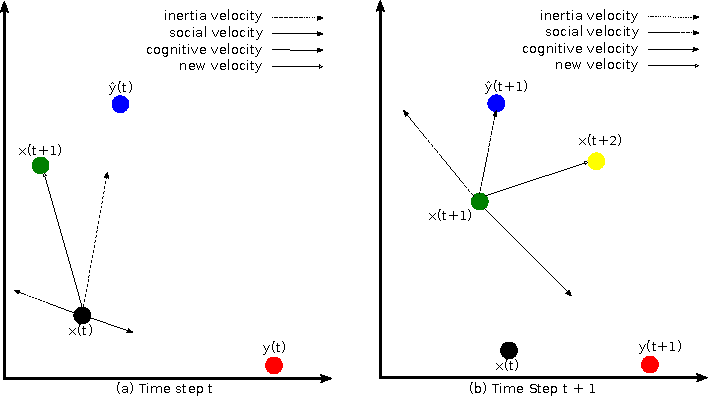
\includegraphics[width=4.5in,height=2.5in]{./pictures/geovelocity.pdf}}
	\caption{Visual particle velocity update \cite{SOSwarm,FundamentalSwarm,CompuIntelligenceIntro,PSOSelfHierarch}}
	\label{fig:particleVelocityUpdate}
	\end{center}
\end{figure}

As discussed earlier gbest is the best position the swarm has occupied since the start of the algorithm. The literature defines that there are two defined methods of determining gbest. The most common method used is where gbest is the best position obtained by a particle in the swarm since the start of the algorithm; thus long-term knowledge dictates the best position found which favours exploitation \cite{CompuIntelligenceIntro,FundamentalSwarm}.
The second method of determining the gbest is the best particle position occupied by any particle in the swarm, in the \emph{current} iteration of the algorithm; thus short-term knowledge dictates the best position found which favours exploration \cite{CompuIntelligenceIntro,FundamentalSwarm}.

Most of the literature has concentrated on the velocity of the particle because it is the main function performing the optimisation. In research done by Ratnaweera \emph{et al.}\cite{PSOSelfHierarch} particle positions in the solutions space are continually monitored. If the particle appears to be stagnant in the search space, the velocity is first updated, and then the particle is reinitialised with a random position. The new position of the particle is then updated with the new velocity, thus knowledge of the discarded particle is retained by using the velocity it had\cite{PSOSelfHierarch}.

In research done by Kalivarapu \emph{et al.} \cite{PSOPheromones} a \gls{PSO} algorithm is developed that seeks to incorporate the pheromone notion of \gls{ACO} algorithms into the velocity updating of particles. The premise of the method is to allow greater sharing of information about promising areas between particles. The algorithm developed by the authors achieved promising results, with it finding solutions faster and also better solutions than other \gls{PSO} algorithms \cite{PSOPheromones}. 

Other research done by Monson and Seppi \cite{adaptPSO} is more concerned with how the particle is presented. In the general \gls{PSO} algorithm, particles have no physical form or volume and so particles in the swarm move through each other. The authors changed this in their algorithm by letting each particle have a radius around itself. This means that as particles move through the search space and another particle at a certain time step occupies that same space, the particles are said to collide. As one would expect, when a collision occurs both particles are deflected into random directions \cite{adaptPSO}. At a greater expense of computational time due to constant collision detection, the \gls{PSO} gains greater exploration in the search space. 

Finally, in the research by Lenin and Monan a \gls{PSO} algorithm is developed that is called the \gls{ARPSO}. The algorithm continually monitors the solutions in the swarm. If it picks up that a certain percentage of the swarm is stagnating, it activates the repulse state. In the repulse state particles are repelled from other particles in the swarm, which facilitates greater exploration. After a certain number of iterations, the algorithm returns to its default state, where particles attract each other. The state of attraction facilitates exploitation \cite{PSOAttractRepulse}.
\subsubsection{Keeping velocity in check}
As can be observed in equation \ref{eq:velocityupdate} the new velocity is added to the old velocity. The velocity of particles can get very large, especially for those particles that are far from the pbest and gbest positions. Large velocities are necessary for early exploration. 

Velocities should be kept in check since if a particles velocity becomes too large, it can overstep the search spaces boundaries and produce infeasible solutions \cite{FundamentalSwarm}. Thus the velocity of a particle needs to be bounded to ensure that its movement with in the search space stays within acceptable bounds. One of the means to bound the velocity is to clamp it. Clamping of velocity is achieved by applying equation \ref{eq:velocityclamp}. The equation is applied on the velocity before its position is updated\cite{FundamentalSwarm}.
\begin{align}
	\hat{v_i}(t+1) &=
	\begin{cases}
	\hat{v'_i}(t+1), &\text{if $\hat{v'_i}(t+1) < \hat{V_{max}}$}\\
	\hat{V_{max}}, &\text{if $\hat{v'_i}(t+1) \geq \hat{V_{max}}$}
	\end{cases} \label{eq:velocityclamp}\\
	\hat{V_{max}} &= \delta(\hat{x_{max}} - \hat{x_{min}})
\end{align}
In equation~\ref{eq:velocityclamp} $\hat{v'_i}$ is calculated using equation~\ref{eq:velocityupdate} for the global \gls{PSO}. Where $\hat{V_{max}}$ is the maximum allowed velocity and $\delta \in (0,1]$. The values $\hat{x_{max}}$ and $\hat{x_{min}}$ are the respective maximum and minimum position vectors in the domain the algorithm is being applied to \cite{FundamentalSwarm}. The value of $\delta$ is very problem dependent and must be carefully chosen to maximise the exploration-exploitation trade-off \cite{FundamentalSwarm}. The use of velocity clamping is not mandatory and should be considered only if the problem requires it\cite{FundamentalSwarm}. Finally there is no guarantee that velocity clamping will prohibit velocities becoming too large\cite{FundamentalSwarm}. There is still a chance, just to a lesser extent\cite{FundamentalSwarm}.

Velocity clamping is not the only developed means by which  the exploration-exploitation trade-off of the \gls{PSO} can be controlled. Consider the case when an object moves with a certain velocity it carries momentum. If the object were to suddenly change direction, momentum would for a certain period still move the object in the previous direction. Inertia weight seeks to add this type of behaviour to the particles of the \gls{PSO} algorithm. The velocity update equation with added inertia is formulated in equation \ref{eq:inertia} \cite{FundamentalSwarm}.
\begin{equation}
\hat{v_i}(t+1) = w\hat{v_i}(t) + c_1\hat{\phi}_1(t)[\hat{pbest}_i - \hat{x}_i(t)] + c_2\hat{\phi}_2(t)[\hat{gbest}_i - \hat{x}_i(t)]\label{eq:inertia}
\end{equation}
Inertia ($w$ in equation \ref{eq:inertia}) was added to the general velocity update equation in an attempt to control the exploration and exploitation of the \gls{PSO} as well as eliminate the need for velocity clamping\cite{FundamentalSwarm}. Although the inertia component did succeed in enabling the control of the \gls{PSO}'s exploration-exploitation in the search space, the need for velocity clamping could not be eliminated\cite{FundamentalSwarm}.

For values of $w > 1$ , the inertia of the particle is increased. With increased inertia the particle will explore more but it is also more likely to leave the boundaries of the search space leading to infeasible solutions \cite{FundamentalSwarm}. 

When $w < 1$ and depending on the values of $c_1$ and $c_2$ each time a particles velocity is updated a certain amount of momentum is lost. The particle seems to slow down, allowing it to exploit the current solution space in finer detail \cite{FundamentalSwarm}. This is not always the case, as $w < 1$ can also lead to the particles in the swarm diverging never to converge on an optimal solution.

To allow for a greater trade-off between exploration and exploitation, the inertia value can be made dynamic. Exploration is favoured early on in an optimisation algorithm and  exploitation later on the algorithm when it is near an optimum. Various methods that are either linear decreasing or non-linear decreasing have been developed that modify the inertia component as the algorithm moves around in the search space \cite{CompuIntelligenceIntro,FundamentalSwarm}.

Finally, a similar inertia type component was developed from the analysis of particle dynamics \cite{FundamentalSwarm}. This new component is called the \emph{constriction coefficient} and, like the inertia above, also modifies the velocity update equation slightly\cite{adaptPSO,FundamentalSwarm,CompuIntelligenceIntro}. 

This modification can be observed in equation~\ref{eq:velocityconstriction}, which is the standard velocity equation with the constriction coefficient. The constriction coefficient is formulated in equation \ref{eq:constriction}\cite{adaptPSO,FundamentalSwarm,CompuIntelligenceIntro}.
\begin{align}
v_i(t+1) &= \chi[v_i(t) + c_1\phi_{1}(t)[pbest - x_i(t)] + c_2\phi_{2}(t)[gbest - x_i(t)]]\label{eq:velocityconstriction}\\
\chi &= \frac{2\kappa}{\lvert 2 - \phi - \sqrt{\phi^2 - 4\phi}\rvert}\label{eq:constriction}
\end{align}

The search constriction coefficient is represented by the value $\phi$. The constriction coefficient evaluates to an ever-decreasing value between $[0,1]$. By using the constriction coefficient the \gls{PSO} algorithm is also guaranteed to converge for values of $\phi \geq 4$ and $\kappa \in [0,1]$. As with the inertia discussed above, high values of $\kappa$ allow for greater exploration and slow convergence, whereas low values of $\kappa$ force the algorithm to exploit the search space and converge quickly \cite{adaptPSO,FundamentalSwarm,CompuIntelligenceIntro}.

\subsubsection{Discrete Value representation}

The \gls{PSO} was developed for continuous valued problem spaces in mind\cite{CompuIntelligenceIntro,FundamentalSwarm}. Fortunately the algorithm has been adapted to a range of problems known as discrete valued problems. These type of problems have the characteristic that the variables contained in the problem domain are finite\cite{CompuIntelligenceIntro,FundamentalSwarm}. Problems that are classified as being of the discrete variant include the \emph{n}-queens problem, the traveling salesman problem and the \gls{FAP}\cite{CompuIntelligenceIntro,FundamentalSwarm}. One of the means by which the \gls{PSO} can be modified to operate in these discrete valued spaces is by changing the representation of position vectors or redefining the operations used for arithmetic such as addition, subtraction and multiplication\cite{CompuIntelligenceIntro,FundamentalSwarm}.

One of the \glspl{PSO} developed that changes the representation of a position vector is the \emph{Binary} \gls{PSO}\cite{CompuIntelligenceIntro,FundamentalSwarm}. Although with the Binary \gls{PSO}, the particles of the swarm operate in binary space, the algorithm can also be applied to real-valued problems since their values can be transformed to fit into the binary space\cite{CompuIntelligenceIntro,FundamentalSwarm}. A consequence of operating in the binary space is that each particles position is represented by $x_{ij} \in {0,1}$\cite{CompuIntelligenceIntro,FundamentalSwarm}. A particle is moved in the binary space by flipping bits in its position vector\cite{CompuIntelligenceIntro,FundamentalSwarm}.

Due to the change in how positions are represented in the binary \gls{PSO} the velocity and trajectory of particles need to be interpreted differently\cite{CompuIntelligenceIntro,FundamentalSwarm}. Velocity is interpreted to represent a probability. A velocity $v_{ij}(t)= 0.4$ defines that the probability that the bit will be 1 is 40\% and the probability that the bit will be 0 is 60\%\cite{CompuIntelligenceIntro,FundamentalSwarm}.

A different and simpler method of applying the \gls{PSO} is by rounding the position to the nearest discrete value\cite{CompuIntelligenceIntro,FundamentalSwarm}. Using this method requires that the position vectors of particles not be outside the bounds of the problem space\cite{CompuIntelligenceIntro,FundamentalSwarm}.

A more complex approach, as mentioned previously, is to redefine the arithmetic operations used when calculating new velocities of particles. In research conducted by Clerc a discrete PSO is applied to the traveling salesman problem, where all the arithmetic operations have been redefined\cite{CompuIntelligenceIntro,FundamentalSwarm}. The traveling salesman problem is defined as follows. Given an $n_x \times n_x$ distance matrix \emph{D}, find a permutation, $\pi$, that minimises the objective function:
\begin{equation}
    \sum^{n_x -1}_{j=1} D_{\pi_j\pi_{j+1}} + D_{\pi_{n_x}\pi_1}
\end{equation}
Clerc redefined the operators as follows:
\begin{itemize}
\item{Velocity of vector length} --- The number of changes to the permutation represented by a tour is defined as the length of the vector\cite{FundamentalSwarm}. Formally the length of the velocity is defined as $|v_i(t)|=J$ where J is the number of elements.
\item{Addition of velocity to a position} --- When velocity is added to a position, a new position is formed\cite{FundamentalSwarm}. A new position represents a new permutation of discrete values and is created by performing swaps on the position and velocity being added\cite{FundamentalSwarm}. Let $x_i$ denote a position and let $v_i$ denote the velocity\cite{FundamentalSwarm}. Then
\begin{equation}
    x_i \oplus v_i = p_i
\end{equation}
where $p_i$ is the new position found by applying the swap operation $v_{i1} = (\pi_{a1},\pi_{b1})$, then for the second swap $v_{i2} = (\pi_{a2},\pi_{b2})$ up and till the last swap\cite{FundamentalSwarm}.
\item{Subtracting positions from each other}  --- The result of subtracting two positions from each other is defined as being a velocity\cite{FundamentalSwarm}. If $x_1$ and $x_2$ are positions and $v$ is the resultant velocity, then
\begin{equation}
x_1 \ominus x_2 = v
\end{equation}
$v$ is defined as such that by applying $v$ to $x_1$ gives $x_2$\cite{FundamentalSwarm}.
\item{Adding two velocities} --- Adding one velocity $v_1$ to another velocity $v_2$ results in a new velocity $v_3$\cite{FundamentalSwarm}. The new velocity $v_3$ is a concatenation of the swaps from $v_1$ and $v_2$ and duplicate swaps are ignored in the new velocity vector\cite{FundamentalSwarm}.
\item{Multiplication of a coefficient to a velocity} --- By multiplying a velocity $v_1$ with a constant $c$ and new velocity is formed. Formally, $v_2 = c \otimes v_1$, where $|v_2| = \lceil c|v_1|\rceil$\cite{FundamentalSwarm}
\end{itemize}

For a more thorough discussion as well as applications of discrete \glspl{PSO} the reader is directed to the survey by Engelbrecht\cite{FundamentalSwarm}. Note that the \gls{FAP} is also a discrete valued problem, the algorithm presented in this research will also need to redefine the standard operators as was done by Cerc for the traveling salesman problem. This redefinition of operators is presented in chapter~\ref{chpt:psoapplicationFAP}.
\subsection{Flow of the Algorithm}
The general concepts that are evident in the \gls{PSO} algorithm have been covered. Using these concepts a general overview will now be given of the \gls{PSO} algorithm flow using algorithm~\ref{alg:PSO} as a reference point. Note that for the algorithm presented a star neighbourhood topology is used and the algorithm is applied on a minimisation problem.
\begin{algorithm}[H]
\caption{Basic Global Particle Swarm Optimisation Algorithm\cite{CompuIntelligenceIntro}}
\label{alg:PSO}
	\begin{algorithmic}[1]
		\State Initialize $s_n$ swarm
		\While{Stopping condition not met}
			\For{each particle $\hat{p_i} \leftarrow 0$ in $s_n$}
				\State Evaluate particle with fitness function $f(\hat{p_i})$
				\If{$f(\hat{p_i}) \leq pbest(\hat{p_i})$}
					\State personal best of $\hat{p_i}$ to $f(\hat{p_i})$
				\EndIf
				\If{$f(\hat{p_i}) \leq f(\hat{gbest)}$}
					\State $\hat{gbest} \leftarrow f(\hat{p_i})$
				\EndIf
			\EndFor
			\For{each particle $\hat{p_i} \leftarrow 0$ in $s_n$}
				\State update velocity of $\hat{p_i}$ with equation~\ref{eq:velocityupdate}
				\State update position of $\hat{p_i}$ with equation~\ref{eq:positionupdate}
			\EndFor
		\EndWhile
	\end{algorithmic}
\end{algorithm}

The \gls{PSO} algorithm starts off by initialising the swarm of particles. Each particle is randomly assigned a certain position in the problem space. After the swarm has been initialised the algorithm enters the optimization or search phase, which starts in line 2.

Before the swarm can start moving around in the problem space, it first needs to determine the gbest particle as well as each particle's own pbest position. Therefore as can be observed in line 3, each particle's current fitness $f(\hat{p_i})$ is determined using a problem-specific fitness function. The fitness determines the lucrativeness of the current position a particle occupies in the problem space.

Once the fitness of a particle's position is calculated, the algorithm needs to determine whether the current position of the particle is its pbest since the algorithm started. This comparison can be seen occur in line 5. 
If the fitness of the currently held position is indeed better than the previous personal best of the particle, then the new position is stored as the personal best for that particular particle, as can be observed in line 6.

Regardless of whether the personal best of a particle has been updated or not, the algorithm performs another comparison also utilising the calculated fitness of the current position of the particle. The algorithm uses this fitness to also determine whether the current position of the particle is the best in the \emph{entire} swarm, i.e whether it is  the \emph{global} best (gbest). This comparison occurs in line  8.
If the position of the particle is indeed the best position in the entire swarm, the algorithm replaces the current gbest with the position of the current particle being evaluated, as seen in line 9.

After the swarm has been evaluated, each particle should have a personal best and the swarm should have a global best. The swarm is therefore ready to move around in the problem space, which occurs in algorithm~\ref{alg:PSO} from lines 12 -- 15.

For each particle in the swarm the algorithm determines the particle's new velocity, as can be observed in line 13. The velocity of a particle is calculated using equation~\ref{eq:velocityupdate}. 

Once the velocity of a specific particle has been calculated, the particle is ready to move to a new position. Moving a particle from its current position to a new position using the calculated velocity is done by applying equation~\ref{eq:positionupdate} and occurs on line 14 of algorithm~\ref{alg:PSO}.

After the whole swarm has been moved, the algorithm continues to the next iteration to evaluate the new positions. This process occurs until certain stopping criteria are met.


\subsection{PSO on the \gls{FAP}}
\label{sec:psoonfap}
The \gls{PSO} algorithm is also a relatively new algorithm and has been applied to only a handful of NP-Complete problems, including the \gls{FAP}. In this dissertation the \gls{PSO} algorithm will be utilized on the \gls{FS-FAP} to try and produce optimal solutions. 

Only two groups have conducted research where the \gls{PSO} has been applied to the \gls{FAP} to produce a near optimal solution. The research concentrated on the \gls{MS-FAP} variant of the \gls{FAP}, and so the aim of their algorithm was to reduce the span of frequencies used. The problem this dissertation is concerned with is the \gls{FS-FAP} where the amount of interference generated needs to be minimised. 

To date, no \gls{PSO} algorithm has been designed to operate on the \gls{FS-FAP} variant. Therefore, the interest in the research mentioned above is more to do with how the authors went about encoding a particular frequency plan as a position for a particle, than with the actual optimisation procedure.

In the research presented by Elkamchouchi \emph{et al.}\cite{EgyptFAPPSO} a \gls{PSO} algorithm is applied to produce optimal solutions for the \gls{MS-FAP}. The way the authors went about assigning frequencies in their algorithm is known as \gls{FEA}.
This method works by first generating a list of calls, called a \emph{call list}, denoting calls that occur in the system\cite{EgyptFAPPSO}. 

The \gls{FEA} method then iterates over the calls in the list and assigns the lowest possible frequencies to the calls without violating interference constraints\cite{EgyptFAPPSO}. The authors note that the specific frequency that is assigned to a particular call depends heavily on the order the calls are in the list\cite{EgyptFAPPSO}.
Due to the success of the \gls{PSO} on the \gls{MS-FAP}, for this dissertation the \gls{PSO} algorithm was selected as the primary means by which to address the \gls{FAP}.

The algorithm also makes extensive use of knowledge gained by the various particles as they search the problem space. Depending on the values used for $w, c_1$ and $c_2$, a particle does not only keep personal history (with pbest), but the swarm as a whole keeps a history of the best particle (neighbourhood best). Thus with regard to \gls{FAP}, it is possible that even though a particle might be in an overall bad position, it might have some small bit of good knowledge being overshadowed by bad knowledge. Through the extensive use of historical knowledge good information is more likely to be shared or kept slightly longer in the algorithms collective knowledge.

For this research the \gls{PSO} was applied to the \gls{FS-FAP} on the \gls{COST} 259 benchmark problems. The approach by the authors in the above literature could not be used. \gls{FS-FAP} is concerned with interference generated and there are some constraints which cannot be broken which are mentioned in section~\ref{sec:COST259} page~\pageref{sec:COST259}. In contrast with \gls{MS-FAP}, the performance measure is explicitly the number of constraints violated not interference.

\section{Summary}
\label{sec:SISummary}
In this chapter three swarm intelligence algorithms were discussed. The general flow of the ant colony optimisation algorithm was described with the help of a pseudo code as well as how the algorithm came about. The defining characteristics of the algorithm were identified and a literature review was given of the \gls{ACO} being applied to the \gls{FAP}.

The second swarm intelligence algorithm was the artificial bee colony optimization algorithm. How the algorithm was developed and how it performs its search in a problem space were explained. A diagram also outlined the general flow of the \gls{ABC} algorithm.

A series of defining characteristics was explained. Each characteristic is a defining attribute of the algorithm that makes it unique with regard to other algorithms. No literature is available on the algorithm being applied to the \gls{FAP} since to date no research has been conducted on such an \gls{ABC} algorithm.

This chapter concluded with the most important algorithm, which is used in this dissertation on the \gls{FAP}, namely the particle swarm optimization algorithm. The flow of the \gls{PSO} algorithm was described in algorithm~\ref{alg:PSO}. Furthermore, characteristics that make the algorithm unique were explained, and a literature review was given of the \gls{PSO} algorithm being applied to the \gls{FAP}.
%Swarm Intelligence
\part{Implementation}
\chapter{PSO on benchmark functions}
\label{chpt:benchmark}
\section{Introduction}
In this section a discussion will be presented on a series of optimisation benchmark functions. First a formulation of all the benchmark functions will be given. In the second section all the benchmark functions will be plotted on a 3d graph. Finally this chapter will conclude with a presentation of the results obtained by the PSO algorithm.

The functions vary from being relatively easy to optimize, to functions that contain lots of local minima and a slightly concealed global minima. In total fourteen benchmark functions will be formulated and benchmarked againts.

If one observed the following research \cite{devparallelgasa,CompuIntelligenceIntro,FundamentalSwarm}. Various optimisation algorithms are benchmarked such as Genetic Algorithm, Artificial Bee Colony algorithm, Tabu Search and Simulated Annealing. In the presented research the algorithms are benchmarked using numerical optimization functions.

Numerical optimization functions are good candidates to test optimisation algorithms as with a few slight changes the function operates in more dimensions or can have more or less optima\cite{devparallelgasa,CompuIntelligenceIntro,FundamentalSwarm}. Being able to alter these functions is a desirable trait as it enables one to accurately benchmark an algorithm, not only with regard to how the algorithm coupes with increased dimensionality but also in the algorithms accuracy in locating optima\cite{devparallelgasa,CompuIntelligenceIntro,FundamentalSwarm}.

The reason why these functions have variable amount of local and global optima, it to test various factors on how good the algorithm is that is being applied on the function. The factors that are tested are\cite{CompuIntelligenceIntro,FundamentalSwarm}:
\begin{itemize}
\item Rate of convergence
\item Exploration
\item Exploitation
\item Diversity
\item Breaking out of local minima
\item Information sharing
\end{itemize}

As discussed previously the numerical functions have predetermined optima, which means researchers are able to produce statistical information on how the algorithm performs. For instance, researchers will not be able to measure accurately the performance of the algorithm on a NP-Complete problem\cite{CompuIntelligenceIntro,FundamentalSwarm}. Yes, they can compare results with what other algorithms have produced, but cannot with absolute certain say or measure the algorithm convergence, diversity etc. on NP-Complete problems as their problem spaces are huge\cite{evalevoalgo}. 

With these benchmark functions, the optima have been mathematically calculated and their position is known within the problem space\cite{evalevoalgo}. Thus, researchers can now with surety measure the convergence rate, diversity and compare it with other algorithms, since the domain the algorithms operate it is not as specific as a NP-Complete problem\cite{evalevoalgo}. Rather, the domain is mathematical and deterministic and therefore allows easy comparison\cite{evalevoalgo}.

In this dissertation, two PSO algorithm were developed specifically to measure the performance of the PSO algorithm and also to better understand the various underlying dynamics of the algorithm.

The first PSO that was developed was just the standard PSO algorithm with no constriction coefficient or inertia weight. The second PSO algorithm differed to the standard algorithm in the sense that it utilizes the notion of inertia to move particles. 

Both of these algorithms have been applied to all fourteen benchmarks that are presented in the chapter and will be compared (where applicable) to other optimisation algorithms that have also been applied to the same benchmark problems. The comparison between these algorithms will be presented in section~\ref{sec:benchResults}.

In the next section, all the benchmarks that will be used for testing the PSO algorithms will be formulated. For the interested reader, 3D graphs along with the python code that generated the graphs are presented in the appendix. This chapter will conclude with a section on the results of the PSO algorithms that were developed being applied to the presented benchmarked as well as compared with other results that have been obtained by other algorithms and presented in the literature.
\section{Test Functions}
In this section all the test functions on which the two developed PSO algorithms will be benchmarked against will be presented. For each test function that is presented a mathematical formulation will be given and the global optimum will be explicitly stated. In addition to the formulation and global optimum, each function will also be classified whether it is a unimodal or modal function as well as whether it is separable or non-separable. Each of these classifications will now be explained.

\begin{description}
\item{\textbf{Unimodal}} --- A particular problem is classified as being unimodal when there is only clear solution. With only one clear solution, it means there is only one global optimum point in the solution space\cite{evalevoalgo,numericalABC,FundamentalSwarm,CompuIntelligenceIntro}.
\item{\textbf{Multimodal}} --- A problem is multimodal when it has more than one defined solution. Thus, the particular problem space contains multiple global optima\cite{evalevoalgo,numericalABC,FundamentalSwarm,CompuIntelligenceIntro}.
\item{\textbf{Separable}} --- Functions that are classified as being separable have the characteristic when the function can be written as a series of summations of just one variable\cite{numericalABC}. This quality makes the function easier to solve as the algorithm has only one variable to be concerned about\cite{evalevoalgo,numericalABC}. Separable functions also have the inherent quality of being scalable, meaning they can be easily be adapted to higher dimensions\cite{evalevoalgo,numericalABC}.
\item{\textbf{Non-separable}} --- Functions classifiied as non-separable cannot be rewritten into a series of summation functions as the variables used in the functions have the characteristic of being interrelated\cite{evalevoalgo,numericalABC}. The interrelation of the variables makes non-separable functions more difficult than separable functions to solve since the algorithm has more interdependent variables to be concerned with\cite{evalevoalgo,numericalABC}.
\end{description}

The De Jong test functions (F1, Shekel's Foxhole) are not considered to be the gold standard of testing optimisation algorithms\cite{evalevoalgo}. The only reason for their extensive use in the literature is due to the functions being the first to be developed and applied to test an optimisation algorithm i.e. Genetic Algorithm\cite{devparallelgasa,evalevoalgo}.

Since the inception of the De Jong test functions, additional functions have been developed which make it more difficult for an optimisation algorithm to locate the optimum\cite{evalevoalgo}. These functions are more difficult in the sense, as they have multiple local optima, which does in actual fact leads the algorithm astray which is to say the problem space is deceptive\cite{CompuIntelligenceIntro,FundamentalSwarm,evalevoalgo}. 

Problems that have deceptive search spaces tests how good the algorithm is resistant to Hill-climbing\footnote{continously selecting what seems to be better moves, but in reality its moving towards a local optima peak} and hence how efficient the algorithm is in exploring the entire search space\cite{evalevoalgo}.
%\textbf{Development of a parallel optimization method based on genetic simulated annealing algorithm}\\
%\textbf{Adaptive Diversity in PSO}\\
%\textbf{A hybrid intelligent genetic algorithm}\\
%\textbf{A Diversity-Guided Particle Swarm Optimizer – the ARPSO}\\
%\textbf{A distributed hierarchical genetic algorithm for efficient optimization and pattern matching}\\
%\textbf{Tabu search for global optimization of continuous functions with application to phase equilibrium calculations}\\
%\textbf{Tabu Search applied to global optimization}\\
%\textbf{On the performance of artificial bee colony (ABC) algorithm}\\
%\textbf{Improving solution characteristics of particle swarm optimization using digital pheromones}\\
%\textbf{Continuous ant colony system and tabu search algorithms hybridized for global minimization of continuous multi-minima functions}\\
%\textbf{Chaotic bee colony algorithms for global numerical optimization}\\
%\textbf{A powerful and efficient algorithm for numerical function optimization: artificial bee colony (ABC) algorithm}\\
%\textbf{A New Quantum Behaved Particle Swarm Optimization}\\
%\textbf{A comparative study of Artificial Bee Colony algorithm}\\
\subsection{DeJong F1 Function}
\begin{equation}
\label{eq:DeJongF1}
	f(x) = \sum_{i=1}^n x^2_i, -5.12 \leq x_i \geq 5.12, i \in \mathbb{N}
\end{equation}
The DeJong F1 Function has the following global minimum when $f(x) = 0, x(i) = 0, i:n$ where $n$ is the amount of dimensions\cite{numericalABC,ABCCompareStudy,ARPSO,PerfABC,ContinACSTS,TestFunctions}. In the literature the function is classified as being unimodal and separable\cite{ABCCompareStudy,TestFunctions}. 
\subsection{Shekel's Foxhole}
\begin{align}
\label{eq:shekel}
	f(x_1,x_2) &= \{0.002 + \sum^{25}_{j=1} [j + (x_1 - a_{1j})^6 + (x_2 - a_{2j})^6]^{-1}\}^{-1}\\
\intertext{where}
	a &= \begin{pmatrix} \nonumber
			-32 & -16 & 0 & 16 & 32 & -32 & ... & 0 & 16 & 32 \\
			-32 & -32 & -32 & -32 & -32 & -16 & ... & 32 & 32 & 32 \\
		 \end{pmatrix}
\end{align}
the variables $x_1$ and $x_2$ are usually restricted to the square represented by $-65.356 \leq x_1 \leq 65.357, -65.357 \leq x_2 \leq 65.356$\cite{ABCCompareStudy,TSGlobalOptimization,ContinACSTS,TestFunctions}. The global optimum is when $f(x_1,x_2) = 0, \{x_1,x_2\} = \{-32,-32\}$\cite{ABCCompareStudy,TSGlobalOptimization,ContinACSTS,TestFunctions}.

The matrix controls the holes that appear in the search space. The interested reader is directed to the 3D graph rendering of this function presented in the appendix on page~\pageref{fig:ShekelGraph} for a visual representation. In the literature the function is classified being multimodal and separable\cite{adaptPSO,ABCCompareStudy,TestFunctions}.
\subsection{Rastrigin}
\begin{equation}
	f(x) = 10n + \sum_{i=1}^n [x_i^2 - 10\cos(2 \pi x_i)],\, i \in \mathbb{N}
\end{equation}
The values of the variable $x_i$ is bounded by the hypercube $-5.12 \leq x_i \leq 5.12$\cite{adaptPSO,ABCCompareStudy,numericalABC,ARPSO,PerfABC,HybridIntelliGA,TestFunctions}. The global optimum for the function is when $f(x_i) = 0,\, x_i = 0, \, i = 1,\dots,n$\cite{adaptPSO,ABCCompareStudy,numericalABC,HybridIntelliGA,TestFunctions}.

Rastrigins function is based on DeJong's first function equation~\ref{eq:DeJongF1} adding a cosine term, which in turns alters the problem space by introducing many local minima\cite{numericalABC,PerfABC,HybridIntelliGA,TestFunctions}. In the literature the function is classified being multimodal and separable\cite{adaptPSO,ABCCompareStudy,numericalABC,ARPSO,ChaoticABC,PerfABC,HybridIntelliGA,TestFunctions}.
\subsection{Schwefel}
\begin{equation}
	f(x) = 418.9829n - \sum^n_{i=1} [x_i\sin{\sqrt{|x_i|}}], \qquad i \in \mathbb{N}
\end{equation}
The variable $x_i$ is restricted to be in the hypercube $-500 \leq x_i \leq 500, i = 1,\ldots,n$\cite{ABCCompareStudy,numericalABC,HybridIntelliGA,DistributedHierarchicalGA,TestFunctions}. The global optimum for the function is $f(x) = 0$ when $x_i = 420.9687$\cite{ABCCompareStudy,numericalABC,HybridIntelliGA,DistributedHierarchicalGA,TestFunctions}. 

If one observes the 3D rendering of the schwefel function problem space on page~\pageref{fig:SchwefelGraph}, one can see that the search space contains a great number of peaks which might be local optima. The function also has the characteristic of having a second best optima far from the global optima which many algorithms get trapped in\cite{ABCCompareStudy,numericalABC,HybridIntelliGA,DistributedHierarchicalGA,TestFunctions}. In the literature the function is classified as being multimodal and separable\cite{ABCCompareStudy,numericalABC,HybridIntelliGA,TestFunctions}.
\subsection{Griewank}
\begin{equation}
	f(x) = \sum^n_{i=1} \frac{x^2_i}{4000} - \prod^n_{i=1}\cos{(\frac{x_i}{\sqrt{i}})} + 1, \qquad i \in \mathbb{N}
\end{equation}
The variable $x_i$ is bounded to within the hypercube $ -600 \leq x_i \leq 600 $\cite{numericalABC,ABCCompareStudy,ARPSO,PerfABC,ContinACSTS,TestFunctions}. The global optimum of the function is when $f(x) =0$ which occurs when $ x_i = 0, i = 1, \dots, n $\cite{numericalABC,ABCCompareStudy,ARPSO,PerfABC,ContinACSTS,TestFunctions}.

As with the schwefel function, the Griewank function also has a great number of peaks and valleys which many algorithm get trapped in. A particular quality of the griewank function is at low dimensions, the function is quite difficult to solve, whereas it has been shown that at higher dimensions the function becomes much easier due to there being less peaks and valleys to navigate in the search space\cite{evalevoalgo,ABCCompareStudy,numericalABC,PerfABC,TestFunctions}. In the literature the function is classified as being multimodal and non-separable\cite{adaptPSO,ABCCompareStudy,numericalABC,ChaoticABC,PerfABC,TestFunctions}.
\subsection{Salomon}
\begin{equation}
	f(x) = -\cos{(2\pi\sum_{i=1}^n\sqrt{x_i^2})} + 0.1 \sqrt{\sum_{i=1}^n x_i^2} + 1, \quad i \in \mathbb{N}
\end{equation}
Unlike the previous functions discussed in this section, the Salomon function imposes no constraint on the $x_i$ variable. The global optimum is when $f(x) = 0$ and $x_i = 0$ where $i = 1,\ldots,n$. This particular function seems to have been applied as benchmarking function yet, as no literature can be found. Nonetheless, the function is indeed a numerical optimisation function that is classified as being multimodal and non-separable\cite{http://www.it.lut.fi/ip/evo/functions/node12.html}.
\subsection{Ackley}
\begin{equation}
	f(x) = -20e^{-0.2\sqrt{\frac{1}{2}\sum_{i=1}^n x_i^2}} - e^{\frac{1}{2}\sum_{i=1}^n\cos{2\pi x_i}} + 20 + e^1, \qquad i \in \mathbb{N}
\end{equation}
The variable $x_i$ is restricted to the hypercube represented by $-32.768 \leq x_i \leq 32.768$\cite{numericalABC,ABCCompareStudy,ARPSO,TestFunctions}. The global minimum is when $f(x) = 0$ and is obtainable for $x_i = 0, i = 1,\ldots,n$\cite{numericalABC,ABCCompareStudy,ARPSO,TestFunctions}.

As can be observed from the mathematical formulation of the function, the function utilizes a exponential term. By using the exponential term the problem space contains numerous local optima which requires an algorithm to search much wider to avoid getting trapped. The literature classifies this function as being multimodal and non-separable\cite{adaptPSO,ABCCompareStudy,numericalABC,TestFunctions}.
\subsection{Six-Hump Camel Back}
\begin{equation}
	f(x_1,x_2) = (4 - 2.1x_1^2 + x_1^{\frac{4}{3}})x_1^2 + (x_1x_2) + (-4 + 4x_2^2)x_2^2
\end{equation}
The variables $x_1$ and $x_2$ are subject to the following boundary constraints $-3 \leq x_1 \leq 3$ and $-2 \leq x_2 \leq 2$\cite{DistributedHierarchicalGA,TestFunctions}. The global minimum is when $f(x_1,x_2) = -1.0316$ and is obtained when $x_1 = -0.0898$ and $x_2 = 0.7126$ or when  $x_1 = 0.0898$ and $x_2 = 0.7126$\cite{DistributedHierarchicalGA,TestFunctions}. 

True to its name the function has six peaks, four of which are local minima and two that are global minima as has already been defined. The literature classifies this function as being multimodal and non-separable\cite{ABCCompareStudy,TestFunctions}.
\subsection{Shubert}
\begin{equation}
	f(x_1,x_2) = -\sum_{i = 1}^5 (i\cos{(i +1)x_1 + 1})\sum_{i=1}^5 (i\cos{(i+1)x_2 + 1})
\end{equation}
The search domain is constrained to $-10 \leq x_i \leq 10, i = 1,2, \ldots, n$\cite{ABCCompareStudy,TSGlobalOptimization,ContinACSTS,TestFunctions}. The global optimum which is when $f(x_i) = -186.7309$\cite{ABCCompareStudy,TSGlobalOptimization,ContinACSTS,TestFunctions}. 

As can be observed from the 3D graph presented in the appendix on page~\pageref{fig:ShubertGraph} the landscape of the Shubert function contains various peaks and slopes. Thus, the function is classified as being multimodal and non-separable\cite{ABCCompareStudy,TestFunctions}.
\subsection{Himmelblau}
\begin{equation}
	f(x_1,x_2) = (x_1^2 + x_2 - 11)^2 + (x_1 + x_2^2 - 7)^2
\end{equation}
The variables $x_1,x_2$ are constraint to be within the hypercube represented by $-6 \leq x_1 \leq 6, -6 \leq x_2 \leq 6$\cite{TestFunctions,ABCCompareStudy}. The Himmelblau function contains no local optima, but on the contrary, it has 4 global optima when $f(x_i) = 0$ which can be obtained at the following points\cite{TestFunctions,ABCCompareStudy}.
\begin{itemize}
\item $(x_1,x_2) = (-3.779310,-3.283185)$
\item $(x_1,x_2) = (-2.805118,3.131312)$
\item $(x_1,x_2) = (3,2)$
\item $(x_1,x_2) = (3.584428,-1.848126)$
\end{itemize}
The literature classifies the function as being multimodal and non-separable\cite{TestFunctions,ABCCompareStudy}.
\subsection{Rosenbrock Valley}
\begin{equation}
	f(x) = \sum_{i=1}^{n-1}[100(x_{i+1} - x_i^2)^2 + (1-x_i)^2
\end{equation}
The variable $x_i$ is bounded to with the following constraint $ -2.048 \leq x_i \leq 2.048 $\cite{numericalABC,ABCCompareStudy,ARPSO,PerfABC,TSGlobalOptContinFunc,HybridIntelliGA}. The global optimum is when $f(x) = 0$ and is obtained when $x_i = 1, i = 1,\ldots,n$\cite{numericalABC,ABCCompareStudy,ARPSO,TSGlobalOptContinFunc,HybridIntelliGA}.

The rosenbrock search space has a curving valley which leads forces algorithms to coupe with the changing direction of the landscape\cite{numericalABC,ABCCompareStudy,ChaoticABC,PerfABC,HybridIntelliGA}. If the algorithm does not adapt to the changing direction it will fail in locating the global optimum. The function is classified as being multimodal and non-separable\cite{numericalABC,ABCCompareStudy,ChaoticABC,PerfABC,HybridIntelliGA}.
\subsection{Dropwave}
\begin{equation}
	f(x) = -\frac{1 + \cos{(12\sqrt{x_1^2 + x_2^2})}}{\frac{1}{2}(x_1^2 + x_2^2) + 2}
\end{equation}
The variables $x_1$ and $x_2$ are restricted to be within the following bounds $-5.12 \leq x_i \leq 5.12$\cite{TestFunctions}. The landscape of this function resembles that of a droplet falling into a pool of water, as can be observed from the 3D graph presented in the appendix on page~\pageref{fig:DropwaveGraph}. Due to its ``wave'' nature, the function has various local minima and only a single optima which is when $f(x_1,x_2) = 0$. The function is classified being multimodal and non-separable\cite{TestFunctions}.
\subsection{Easom}
\begin{equation}
	f(x_1,x_2) = -\cos(x_1)\cos(x_2)e^{(-(x_1 - \pi)^2 - (x_2 - \pi)^2)}
\end{equation}
The variables $x_1$ and $x_2$ are restricted to be within the hypercube represented by $-100 \leq x_1 \leq 100, -100 \leq x_2 \leq 100$\cite{TSGlobalOptContinFunc,ContinACSTS,TestFunctions}. The global minimum is when $f(x_1,x_2) = -1$ and is obtainable if $(x_1,x_2) = (\pi,\pi)$\cite{TSGlobalOptContinFunc,ContinACSTS,TestFunctions}. 

The easom function has a deceptive global minimum as it is very close to other local minima\cite{ABCCompareStudy,TSGlobalOptimization}. As can be observed from the 3D graph of the function on page~\pageref{fig:EasomGraph}, the search space is a flat with the global minima clearly visible. Flat search spaces are difficult to navigate by algorithms as the surrounding area gives no indication whether the algorithm is on the right track of not. The function is classied as being multimodal and non-separable in the literature \cite{ABCCompareStudy,TSGlobalOptimization,TSGlobalOptContinFunc}.
\subsection{Branins}
\begin{align}
	f(x_1,x_2) &= a(x_2 - bx_1^2 + cx_1 - d)^2 + e(1-f)\cos{x_1} + e \\
\intertext{where}
	a &= 1\nonumber\\
	b &= \frac{5.1}{4\pi^2}\nonumber\\
	c &= \frac{5}{\pi}\nonumber\\
	d &= 6\nonumber\\
	e &= 10\nonumber\\
	f &= \frac{1}{8\pi}\nonumber
\end{align}
The variables $x_1$ and $x_2$ are subject to the following boundary constraints $-5\leq x_1 \leq 10, 0 \leq x_2 \leq 10$\cite{ABCCompareStudy,TSGlobalOptimization,ContinACSTS,TestFunctions}. The global optimum is when $f(x_1,x_2) = 0.397887$ and is obtainable when $x_1$ and $x_2$ have the following values\cite{ABCCompareStudy,TSGlobalOptimization,ContinACSTS,TestFunctions}:
\begin{enumerate}
\item $x_1 = -\pi,\:x_2=12.275$
\item $x_1 = \pi,\:x_2=2.275$
\item $x_1 = 9.42478,\:x_2=2.475$
\end{enumerate}
The literature classifies this function as being multimodal and separable\cite{ABCCompareStudy,TSGlobalOptimization,ContinACSTS,TestFunctions}.
\subsection{Michalewicz}
\begin{equation}
	f(x) = -\sum_{i=1}^n\sin{(x_i)}[\sin{(\frac{(1 - x_i^2)}{\pi})}]^{2m}, \qquad i,m \in \mathbb{N}
\end{equation}
The variable $x_i$ is usually constricted to the following defined boundary $0 \leq x_i \leq \pi, i = 1,\ldots,n$\cite{ABCCompareStudy,TestFunctions}. The parameter $m$ defines the steepness of the valleys in the function. The function has two approximated global minima's that are difficult to locate since their size in comparison to the rest of the search space is relatively small\cite{ABCCompareStudy,TestFunctions}.
%http://www.geatbx.com/docu/fcnindex-01.html#P216_11735
\begin{enumerate}
\item $f(x) = -4.687,\: n = 5$
\item $f(x) = -9.66,\: n = 10$
\end{enumerate}
In the literature the function is classified as being multimodal and separable\cite{ABCCompareStudy}.
\subsection{Goldstein}
\begin{align}
	f(x_1,x_2) &= (1 + (x_1 + x_2 + 1)^2)\nonumber\\
			   &=*(19-14x_1+3x_1^2 -14x_2 + 6x_1x_2 + 3x_2^2)\nonumber\\
			   &=*(30 + (2x_1 -3x_2)^2\nonumber\\
			   &=*(18 - 32x_1 + 12x_1^2 +48x_2 -36x_1x_2 + 27x_2)\nonumber
\end{align}
The variables $x_1$ and $x_2$ are subject to the following boundary constraints $-2 \leq x_1 \leq 2, -2 \leq x_2 \leq 2$\cite{ABCCompareStudy,TSGlobalOptimization,TSGlobalOptContinFunc,ContinACSTS,TestFunctions}. The function has only one global minimum four local optima\cite{ABCCompareStudy,TSGlobalOptimization}. The global optimum is when $f(x_1,x_2) = 3$ and is obtainable when $x_1 = 0$ and $x_2 = -1$\cite{ABCCompareStudy,TSGlobalOptimization,TSGlobalOptContinFunc,ContinACSTS,TestFunctions}.

The literature classifies this function as being multimodal and non-separable\cite{ABCCompareStudy}.

\section{Results}
\label{sec:benchResults}
In the previous section sixteen benchmark functions were mathematically defined, where applicable comments were given on the search space. For each function the following was explicitly stated:
\begin{itemize}
\item The global optimum and where is located.
\item Whether the function is unimodal or multimodal.
\item Whether the function is non-separable or separable.
\end{itemize}
In this section the results will be presented of how the two PSO algorithms that were developed performed on each of the presented benchmark functions. 

The algorithms will be compared with the following criteria on each benchmark.
\begin{itemize}
\item The number of iterations the algorithm took to find the global optimum
\item The accuracy of the algorithm, which means if the algorithm has indeed located the optimum or if not, how far off is the algorithm.
\item The PSO is a population-based algorithm, thus diversity is important. Diversity will be measured and compared on each benchmark function.
\end{itemize}
For each of the above criteria a subsection will be presented. Where possible the results obtained will be compared to other algorithms that have been applied to similar test functions.

\subsection{Fina values}
\begin{center}
	\begin{tabular}{| c | c | c | c | c | c |}
	\hline
	Function & PSO & PSO* & GA & TS & ABC\\  \hline
	DeJong F1 & 0 & -- & -- & -- & --\\ \hline
	Shekel's Foxhole & 0 & -- & -- & -- & --\\ \hline
	Rastrigin & 0.74622 & -- & N/A & N/A & N/A\\ \hline
	Schwefel & -1.19069e+43 & -- & N/A & N/A & N/A\\ \hline
	Griewank & 1.00003 & -- & N/A & N/A & N/A\\ \hline
	Salomon & -0.460561 & -- & -- & -- & --\\ \hline
	Ackley & -4.5901 & -- & N/A & N/A & N/A\\ \hline
	Six-Hump camelback & -1.03163 & -- & -- & -- & --\\ \hline
	Shubert & -186.731 & -- & -- & -- & --\\ \hline
	Himmelblau & 1.02103 & -- & -- & -- & --\\ \hline
	RosenbrockValley & 1.81101e-08 & -- & -- & -- & --\\ \hline
	Dropwave & 4.59843e-15 & -- & -- & -- & --\\ \hline
	Easom & -1 & -- & -- & -- & --\\ \hline
	Branins & 1.22875 & -- & N/A & N/A & N/A\\ \hline
	Michalewicz & -2.40391 & -- & -- & -- & --\\ \hline
	Goldstein & infinity & -- & -- & -- & --\\ \hline
	\end{tabular}
\end{center}
\subsection{Diversity}
\begin{center}
	\begin{tabular}{| c | c | c | c | c | c |}
	\hline
	Function & PSO & PSO* & GA & TS & ABC\\  \hline
	DeJong F1 & -- & -- & -- & -- & --\\ \hline
	Shekel's Foxhole & -- & -- & -- & -- & --\\ \hline
	Rastrigin & -- & -- & -- & -- & --\\ \hline
	Schwefel & -- & -- & -- & -- & --\\ \hline
	Griewank & -- & -- & -- & -- & --\\ \hline
	Salomon & -- & -- & -- & -- & --\\ \hline
	Ackley & -- & -- & -- & -- & --\\ \hline
	Six-Hump camelback & -- & -- & -- & -- & --\\ \hline
	Shubert & -- & -- & -- & -- & --\\ \hline
	Himmelblau & -- & -- & -- & -- & --\\ \hline
	RosenbrockValley & -- & -- & -- & -- & --\\ \hline
	Dropwave & -- & -- & -- & -- & --\\ \hline
	Easom & -- & -- & -- & -- & --\\ \hline
	Branins & -- & -- & -- & -- & --\\ \hline
	Michalewicz & -- & -- & -- & -- & --\\ \hline
	Goldstein & -- & -- & -- & -- & --\\ \hline
	\end{tabular}
\end{center}
\subsection{Accuracy}
\begin{center}
	\begin{tabular}{| c | c | c | c | c | c |}
	\hline
	Function & PSO & PSO* & GA & TS & ABC\\  \hline
	DeJong F1 & -- & -- & -- & -- & --\\ \hline
	Shekel's Foxhole & -- & -- & -- & -- & --\\ \hline
	Rastrigin & -- & -- & -- & -- & --\\ \hline
	Schwefel & -- & -- & -- & -- & --\\ \hline
	Griewank & -- & -- & -- & -- & --\\ \hline
	Salomon & -- & -- & -- & -- & --\\ \hline
	Ackley & -- & -- & -- & -- & --\\ \hline
	Six-Hump camelback & -- & -- & -- & -- & --\\ \hline
	Shubert & -- & -- & -- & -- & --\\ \hline
	Himmelblau & -- & -- & -- & -- & --\\ \hline
	RosenbrockValley & -- & -- & -- & -- & --\\ \hline
	Dropwave & -- & -- & -- & -- & --\\ \hline
	Easom & -- & -- & -- & -- & --\\ \hline
	Branins & -- & -- & -- & -- & --\\ \hline
	Michalewicz & -- & -- & -- & -- & --\\ \hline
	Goldstein & -- & -- & -- & -- & --\\ \hline
	\end{tabular}
\end{center}

\section{Summary}
In this chapter a series of mathimatical optimisation problems were presented. Each problem was mathematically formulated as well as categorised as to whether the particular problem is multi-modal and seperable.

To get a better idea on how the Particle Swarm Optimisation (PSO) algorithm operates and performs two PSO algortihms were developed. The first PSO algorithm uses the standard velocity equation with no alterations. The second PSO algorithm uses the notion of inertia with regard to velocity calculation.

The algorithms that were developed were tested on all the mathematical problems outlined at the start of this chapter. The chapter concluded with a presentation of the results obtained by the algorithms along with a short discussion on the obtained results.
%PSO on benchmark functions
\chapter{Applying the PSO to the FAP}
\label{chpt:psoapplicationFAP}
\section{Introduction}
PSO, as discussed previously (see page \pageref{sec:PSO}), is an algorithm that is largely based on the flying behaviour exhibited by a flock of birds. This is why the core of the algorithm is based upon vector mathematics, with new positions and velocities being calculated after each iteration of the algorithm. Thus a D-dimensional vector represents each particle position and is then simulated by flying through the D-dimensional space using the velocity equation (see section~\ref{sec:particleVelocity} on page~\pageref{eq:velocityupdate}).

Most of the problems to which \gls{PSO} has been applied to date have been problems where the position of particles has a constant D-dimensional space. This constant dimensionality introduces an intriguing problem if one wants to apply the \gls{PSO} to an inherent multidimensional problem like the \gls{FAP}. This chapter deals with how the \gls{PSO} was applied to the \gls{FAP}.

Firstly, the particle position is represented in the frequency planning domain is defined. This definition of the particle position is important because it plays a central part in the movement of particles through the frequency planning domain. A description is then given of how each position is evaluated as well as the fitness function that the \gls{PSO} will use in the \gls{FAP} domain.

Arguably the most important part of the swarm is how the velocity of a particle is calculated and then moving it to a new position in the problem space. The velocity update is important, as it is the primary means by which the algorithm searches the problem space.

As was discussed in section~\ref{sec:psoonfap}, applying the \gls{PSO} to the \gls{FAP} introduces a variety of challenges. One of the challenges is how exactly one moves a frequency plan towards another frequency plan. This is an important question that needs to be addressed as the \gls{PSO} algorithms have no other way of searching the problem space by any other means.

As mentioned in the previous chapter the FAP is a discrete valued problem and for the \gls{PSO} to operate in the \gls{FAP} space custom operators (called velocity functions in this discussion) had to be developed to enable the particles of the swarm to move. These velocity functions are discussed in section~\ref{sec:velocityFAP}. 

Developing custom velocity functions for the \gls{PSO} was simply not enough to achieve good results with the \gls{PSO} . Therefore more innovations needed to be made to improve the solution quality of the \gls{PSO} . In section~\ref{sec:buildglobalbest} a new mechanism is presented for selecting the global best which enabled the \gls{PSO} to get better fitness values and therefore direct the swarm more towards better solutions. Finally, the chapter will conclude with how the swarm utilises history to produce better results to enable the \gls{PSO} to further improve the solution quality.
\section{Position in the Frequency Planning Domain}
This section presents a description on what a position is in the frequency planning domain. First a frequency plan is defined and the general structure to represent such a plan is provided. The section will conclude with the hard and soft constraints and how the constraints aid in creating a frequency plan that is suitable for a network.

A frequency plan, is almost exactly what the name implies: A plan that outlines frequency usage for a mobile telecommunication network. The benchmark problems that were used to test the developed \gls{PSO} all pertained to cellular phone networks and were presented in section~\ref{sec:FAPBenchmarks}. For cellular networks, the frequency plan outlines which frequency must be allocated to which transceiver. With this basic definition, the problem is deceptive as one naturally assumes that there are an infinite number of frequencies that can be used or the number of frequencies available for assignment is more than the number of transceivers in the network. 

The reality is that there are only a finite number of frequencies available for cellphone transmissions, as was discussed in chapters~\ref{chpt:celltech} and \ref{chpt:fap}. Hence a regulatory body needs to assign wireless spectrum to cellphone network operators for use in their networks. A regulatory body is needed because, if a network operator uses just any frequency it wants, it is bound to interfere with someone else also utilising the same frequency.

A network is not assigned to the entire wireless spectrum for wireless communication, but rather only a subset is assigned to the network. If one observes the \gls{FAP} benchmark problems the \gls{PSO} was applied to (see section~\ref{sec:FAPBenchmarks}) for instance Siemens1, the allotted spectrum is from frequency 16 to 90. Which gives the network operator 74 frequencies to use in its network without considering other constraints. 

Besides the electromagnetic constraints that are also applicable here, there are regulatory constraints, for instance frequencies in the spectrum that are by no means allowed to be used. These frequencies are referred to as globally blocked frequencies and are hard constraints. An in-depth discussion of these constraints was given in section~\ref{sec:Interference}. As discussed in chapters~\ref{chpt:celltech} and \ref{chpt:fap}, a cellphone network is divided into a number of cells, and each cell requires a certain number of transceivers to service its corresponding area. 

The number of transceivers is based on the expected volume of traffic that a particular cell will experience at peak network usage. Some cells might be located in highly populous areas, which means the potential traffic that cell might need to handle during peak network usage is very high and thus the cell has more than one transceiver to handle the potential traffic. With cells that are located in areas that have a low population, the potential traffic the cell might experience during peak network usage is low and thus the cell only has one transceiver to handle potential traffic.

Based on the amount of traffic a cell needs to handle, the number of transceivers differs; thus in a frequency plan not all cells have the same number of transceivers, otherwise a frequency plan can be modelled as a series of constant D-dimensional vectors, where the D represents the number of transceivers. 
\begin{figure}[ht]
	\centering
	\setlength \fboxsep{0pt}
	\setlength \fboxrule{0.5pt}
	\fbox{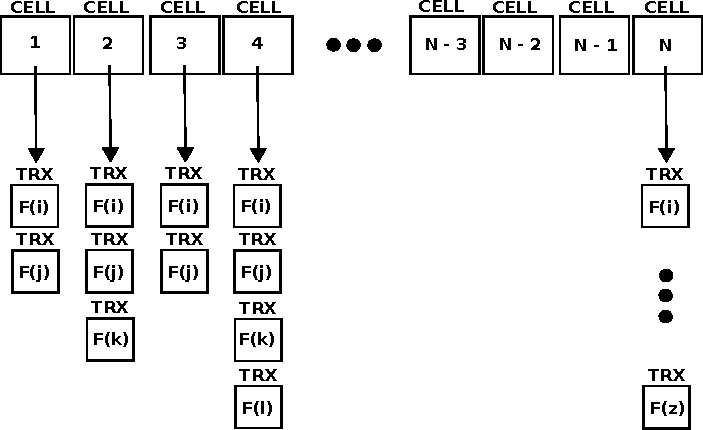
\includegraphics[width=4.8in, height=3.5in]{./pictures/fapPlanDiagram.pdf}}
	\caption{The structure of a frequency plan}
	\label{fig:fapPlan}
\end{figure}
As can be seen in figure \ref{fig:fapPlan} a cellular network can have any number ($N$ in the figure) of cells to attain the desired coverage over the geographical landscape. In the COST 259 benchmark problems the cellular networks have a large number of cells that range from 500 to more than 1000. 

The most important part of the plan is the actual transceivers within each cell. In figure~\ref{fig:fapPlan} it can be clearly seen how the number of transceivers (TRXs) varies from one cell to the next. $F(i)$ is a frequency at position $i$ from the available usable spectrum. 

Based on the structure of the plan depicted in figure \ref{fig:fapPlan} there is no concept of which cell interferes with which other cell and if there is indeed interference; the amount of interference that is experienced. Not all this information is part of the plan. Instead this information, for the purpose of this research is supplied by the COST 259 benchmark. 

The interference information is referred to as the interference matrix. A definition of the structure of an interference matrix was given in section~\ref{sec:Interference}. As discussed, each entry references two cells' entries: Cell A and Cell B. Along with the entry the amount of interference that occurs when Cell B interferes with Cell A is also listed.

A frequency plan is a possible solution to the \gls{FAP}. Therefore in the \gls{PSO} that was developed each particle's position in the solution space is represented by a frequency plan. As illustrated in figure~\ref{fig:fapPlan}, a frequency plan is just a series of cells, where each cell has a set of transceivers; thus in the \gls{PSO} algorithm a plan is actually represented as an array of cells. This enables the algorithm to access particular cells in a plan by index as can be observed in listed algorithms~\ref{alg:velocitymethod1} and ~\ref{alg:velocitymethod2}. 

Before the particles can actually start to move around in the \gls{FAP} space, they first need to be assigned positions. In the developed \gls{PSO} listed in algorithm~\ref{alg:FAPPSO} line 1 the first operation that the algorithm executes is to initialise all the particles in the swarm. A particle position in the algorithm is initialised by assigning it a random position; thus a frequency plan (representing a position) is randomly generated by the algorithm.
\begin{algorithm}[H]
\caption{The \gls{FAP} \gls{PSO} Algorithm}
\label{alg:FAPPSO}
\begin{algorithmic}
\State $s_n$ = Initialize Swarm $s_n$
\While{Termination criterion not met}
	\State EvaluateSwarm($s_n$)
	\State UpdateGlobalBest($s_n$)
	\State UpdateSwarmMovement($s_n$,$gbest$)
\EndWhile
\end{algorithmic}
\end{algorithm}

The position is purely random in that the only considerations made by the position generator are that valid frequencies are assigned to transceivers installed at cells. Thus the generator does not check whether a frequency has already been assigned in the current cell or any other considerations. The intended purpose of the generator is just to place a particle in the problem space, not the premature start of the optimisation process.

Since particles are able to occupy positions in the \gls{FAP} space the \gls{PSO} algorithm is now able to move them around in the problem space. As mentioned previously, moving particles through the frequency plan solution space introduces an interesting problem due to the multidimensionality of a plan. 

A discussion of how particles are moved from one position to another through the solution space is provided in section \ref{sec:velocityFAP}. The next section presents an explanation on the fitness function that determines the desirability of a particular particle's position or rather the frequency plan its position represents.
\section{The Fitness Function}
The fitness function rates the desirability of a particular particle's position in the problem space. As discussed in the previous section, the COST 259 benchmark problems provide an interference matrix that lists the total amount of interference that occurs when a pair of cells interfere. As outlined in the structure definition (see section~\ref{sec:Interference}) each entry in the interference matrix defines a pair of cells that are said to interfere, along with two additional values. 

The first value is referred to as co-channel interference and is the total amount of interference that will occur on the communication link when the allocated frequency of one transceiver, is equal to a transceiver in the other cell that is listed in the interference matrix. The second value is called adjacent channel interference and it is the total amount of interference that will occur on the communication link when the allocated frequency of a transceiver, in one cell, differs by 1 from another frequency allocated to the transceiver from the other cell that is listed in the interference matrix.

Particles move towards other particles because the other particles have indicated (through information sharing) that the positions they occupy are very lucrative and thus they have found potentially good solutions. The particles in the developed \gls{PSO} share information based on the star social network structure. The only way particles can know the lucrativeness of the position they occupy is if the position is evaluated with a fitness function. Thus the lucrativeness of a position is actually the fitness value obtained from the fitness function.

Since a particle position is defined as a frequency plan, a procedure is needed that calculates the fitness of a frequency plan. With the \gls{FS-FAP} the primary concern is to keep interference to a minimum. Therefore in the \gls{PSO} that was developed the fitness value is the total amount of interference generated by all the cells with their allocated frequencies. 

The evaluation procedure goes through each pair of cells defined in the interference matrix where it looks up both cells in the frequency plan. The second cell is said to interfere with the first cell. Therefore each transceiver in the first cell is checked against all the transceivers of the other cell. Depending on whether the frequencies differ from each other, the fitness procedure adds either co-channel or the adjacent channel interference to a summing variable. This procedure is mathematically defined in chapter 3 (see page \pageref{E:costFunction} for the formal equation) and algorithm~\ref{alg:fapcost} is the pseudo code of the implemented equation used by the \gls{PSO} . 

\begin{algorithm}
\caption{FAP Cost Function}
\label{alg:fapcost}
	\begin{algorithmic}[1]
	\Require normalCell
	\Require interferingCell
	\State $totalInterference \leftarrow $0
	\For{Each TRX $trx_i$ in interferingCell}
		\For{Each TRX $trx_j$ in normalCell}
			\State $interference \leftarrow 0$
			\State $difference \leftarrow$ $|trx_i - trx_j|$
			\If{difference is 0}
            \If{\emph{coChannelInterference} $\leq$ \emph{minInterferenceThershold}}
					\State $interference \leftarrow interference + 0$
				\Else
                \State \emph{interference} $\leftarrow$ \emph{interference} + \emph{coChannelInterference}
				\EndIf
			\Else
            \If{difference is 1}
                \If{\emph{adjChannelInterference} $\leq$ \emph{minInterferenceThershold}}
                    \State \emph{interference} $\leftarrow$ \emph{interference} + 0
					\Else
                    \State \emph{interference} $\leftarrow$ \emph{interference} + \emph{adjChannelInterference}
					\EndIf
				\EndIf
			\EndIf
            \State \emph{totalInterference} $\leftarrow$ \emph{totalInterference} + \emph{interference}
		\EndFor
	\EndFor
	\end{algorithmic}
\end{algorithm}

As can be seen in algorithm~\ref{alg:fapcost} not all interference values are added to the total amount of interference variable. The COST 259 benchmarks define a minimum tolerable interference variable. This means that if a given interference value is either equal to or less than this defined value the interference generated is negligible and can be disregarded as it will not have a noticeable impact on the communication link. The following section discusses how particles are moved from one iteration to the next using frequency plans as positions in the solution space.
\section{Velocity Function for Frequency Planning}
\label{sec:velocityFAP}
The velocity function is arguably the core of the \gls{PSO} algorithm. It is the procedure by which particles in the swarm move from one point to another in the solution space. 

The velocity function does not blindly move a particle from one point to another, but instead it takes the particle history into account as well as the best particle in the swarm. Therefore the velocity function is the core means by which the swarm explores the solution space. A more thorough explanation is provided in section~\ref{sec:particleVelocity}.

The development of a velocity function that is suitable for particles to move from one frequency plan to another is covered next. The section will start off with the first velocity function that was developed. With each method discussed, the problems associated with it will also be mentioned. This section will conclude with the second method that was developed and that is also the primary method the developed \gls{PSO} uses.

\subsection{Movement in the Frequency Planning Domain}
The standard velocity equation works on the basis of vector mathematics. Each particle has a velocity and position, which is represented by a standard mathematical vector. The standard equation alters the direction of the particle to move to a more promising position in the solution space that is in the general direction of the global best particle and a previous personal best position the particle held..

Vector mathematics has standard basic operations defined for adding, subtracting and multiplying; hence applying the \gls{PSO} to problems that are either mathematical functions or problems that map well to the vector domain is a defined process. With regard to the frequency planning domain an important question needs to be answered: How can one multidimension frequency plan be moved to another?

With any difficult problem it is better to break the problem down into its most basic constructs and then solve each piece individually until the problem as a collective is solved. This technique is also commonly known as divide and conquer. This technique was first applied to the nature of a frequency plan.

A frequency plan is a plan that consists of a series of different cells that are in use in the network. The plan specifies the frequencies that each individual transceiver installed at a cell must use for communication. Thus a frequency plan can be broken up into three important constructs:
\begin{enumerate}
\item A plan is a list of different cells.
\item Each cell in a plan has a list of transceivers that it has installed.
\item Each installed transceiver has a single number allocated to it called the frequency. This frequency is used for communication.
\end{enumerate}

As discussed previously, a position is a frequency plan and each particle has a current position and a best position. A visual depiction of a particle position is presented in figure~\ref{fig:fapparticlepos}. The global best particle is also depicted in the figure. When providing examples on how any of the following velocity methods operate, figure~\ref{fig:fapparticlepos} will be used as reference point.
\begin{figure}[ht]
	\centering
	\setlength \fboxsep{0pt}
	\setlength \fboxrule{0.5pt}
	\fbox{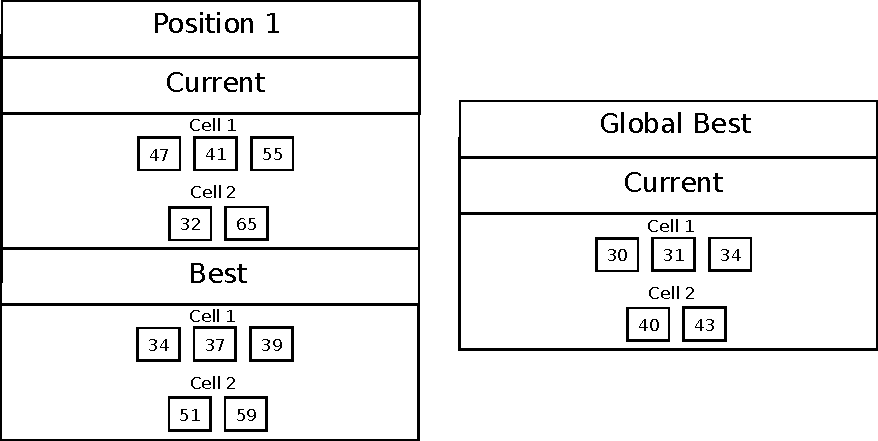
\includegraphics[width=4.8in, height=3.5in]{./pictures/FAP_Particle_Positions.pdf}}
	\caption{FAP PSO Particle Position and Global Best Position}
	\label{fig:fapparticlepos}
\end{figure}

Now that a frequency plan has been broken up into its constructs, the question of how to move one frequency plan to another can be rephrased. How does one move a frequency allocated to a \emph{transceiver} in a particular \emph{cell} of one frequency plan to another frequency of the \emph{same} transceiver and cell in another \emph{different} plan? An important realisation needs to be noted here. In the \gls{PSO} at any one time the algorithm is only considering two positions and for the \gls{FAP} the two positions are frequency plans. Both plans are \emph{identical} except for the specific frequencies that transceivers use. Thus a cell that exists in the one plan, also exists in another plan. Both the cells have exactly the same number of transceivers installed; only the frequencies each individual transceiver uses for communication differ.

Using this realisation, the conclusion can be made that the velocity equation can only work with the frequencies assigned to transceivers. Therefore a potential velocity equation mechanism needs to operate on the finest granularity of a frequency plan, i.e. the frequencies.

The principle on which the first velocity method developed is based, is for the movement of the swarm to be at a much finer granularity and hence movement is based on frequencies. Therefore when a particle needs to move towards a global best particle, the velocity procedure goes into the intricate details of the particle wanting to move and the global best particle. The procedure goes into each cell defined in the frequency plan represented by the standard particle as well as the global best particle to be able to access each installed transceiver.

To be able to move from one frequency plan to another by utilising the standard velocity equation, the equation needs to be broken up into its smaller operations. In this way, small operations can be developed that perform the same function as the individual parts. The velocity equation in section~\ref{sec:particleVelocity} can be broken up into the following parts:
\label{lst:velocitybreakup}
\begin{itemize}
\item \textbf{Subtraction} \\SubtractionResultPbest: $pbest - x_i(t)$\\SubtractionResultGbest: $gbest - x_i(t)$
\\
\item \textbf{Multiplication} \\MultiPbestResult: $c_1\phi_1 * SubtractionResultPbest$\\MultiGBestResult: $c_2\phi_2 * SubtractionResultGbest$ 
\item \textbf{Addition}\\$v_i(t) + MultiPbestResult + MultiGBestResult$
\end{itemize}
There are no mathematical constructs that define how two frequency plans are added together or subtracted, let alone multiplied. As discussed earlier, a frequency plan is just a series of cells that have frequencies. These frequencies are numbers that internally are just integers and there are mathematical constructs that define how two integers should be added, subtracted or multiplied. Both velocity methods that were developed utilise the basic principle that on a fine granularity of a frequency plan one is merely working with integers.


The first velocity method is listed in algorithm~\ref{alg:velocitymethod1}. Velocity method 1 works on the principle of moving one cell in a particular frequency plan to the same cell in a different frequency plan. As noted earlier, the cells are the \emph{same}, but the frequencies that have been allocated to each transceiver within a cell differ. Thus in velocity method 1, each cell has an array of transceivers. The array of transceivers contains the individual frequency numbers that have been allocated to a cell.

Before the algorithm is presented, the operations used for addition, subtraction, multiplication and multiplication with a scalar needs to be defined. The following equations formulate all of these operations and are used by Velocity method 1.
\begin{align}
    \Delta c_{ij} &= f(c^1_{ij}) + f(c^2_{ij})\label{eq:arrayAdd}\\
    \Delta c_{ij} &= f(c^1_{ij}) - f(c^2_{ij})\label{eq:arraySubtract}\\
	\Delta c_{ij} &= f(c^1_{ij}) * f(c^2_{ij})\label{eq:arrayMultiply}\\
    \Delta c_{ij} &= f(c_{ij}) * s \label{eq:arrayScalar}\\
    \text{where, }c &\in \{c_{00},c_{01},c_{10}, \dots, c_{ij}\} , \forall i,j,s \in \mathbb{N}, i \leq \text{MaxCells}, j \leq t(c_i)\nonumber\\ 
    p_i &\in \{\{c_{01},c_{02},\dots,c_{ij}\}_1,\{c_{01},c_{02},\dots,c_{ij}\}_2, \dots,\{c_{01},c_{02},\dots,c_{ij}\}_k\}\nonumber
\end{align}
In the above equations $c^1$ and $c^2$ represent different frequencies plan positions. The function $f$ retrieves the frequency assigned to a TRX $c_{ij}$. MaxCells is the maximum amount of cells in the frequency plan. The function $t$ retrieves the total amount of TRXs installed at a particular cell $c_i$. The variable $s$ in equation~\ref{eq:arrayScalar} is any scalar value. The variable $p_i$ represents a particle in the swarm and $k$ is the max swarm size. Now that all the equations have been defined, the algorithm can be represented. 

Velocity method 1 is depicted in algorithm~\ref{alg:velocitymethod1}. The algorithm moves one array of transceivers to another array of transceivers. The variable $r$ in algorithm~\ref{alg:velocitymethod1} below is a random scalar value. In each of the equations the particular arithmetic operation is applied to the same TRX found in both frequency plans. The first method that is used to calculate the velocity of a frequency plan, is the first basic operation defined in the velocity equation, namely subtraction, and utilises equation~\ref{eq:arraySubtract}.
\begin{algorithm}[H]
\caption{Velocity Method 1}
\label{alg:velocitymethod1}
	\begin{algorithmic}[1]
        \Require currentParticle -- The particle that needs to move (\emph{fromPosition})
        \Require globalBestParticle -- The particle to move towards (\emph{toPosition})
	\State $pbest \leftarrow $Particle best position
	\State $gbest \leftarrow $globalBestParticle position
	\State $pBestSubtractResult \leftarrow currentParticle - pbest$ with equation~\ref{eq:arraySubtract}
	\State $gBestSubtractResult \leftarrow currentParticle - gbest$  with equation~\ref{eq:arraySubtract}
    \State $a \leftarrow localCoeff \times pBestSubtractResult \times r$ using equation~\ref{eq:arrayMultiply} and~\ref{eq:arrayScalar}
    \State $b \leftarrow globalCoeff \times gBestSubtractResult \times r$  using equation~\ref{eq:arrayMultiply} and~\ref{eq:arrayScalar}
	\If{first time velocity is calculated for current Particle}
		\State $v \leftarrow a + b$ using equation~\ref{eq:arrayAdd}
	\Else
		\State $abAdditionResult \leftarrow a + b$ using equation~\ref{eq:arrayScalar}
		\State $v' \leftarrow abAdditionResult + v$ using equation~\ref{eq:arrayAdd}
		\State $v \leftarrow w \times v'$ using equation~\ref{eq:arrayScalar}
	\EndIf
	\State $currentParticle \leftarrow v + currentParticle$ using equation~\ref{eq:arrayAdd}
	\State SanatizePosition(currentParticle)
	\end{algorithmic}
\end{algorithm}

To better understand how velocity method 1 operates. An example will now be presented using figure~\ref{fig:fapparticlepos} as the example position and example global best. Note that for the example presented, only $cell_1$ is considered for the current, personal and global best position. The example is verbose to better illustrate the workings of the method.
\begin{align}
    pbest_1 &= \{34,37,39\} \nonumber \\
    gbest_1 &= \{30,31,34\} \nonumber \\
    cell_1 &= \{47,41,55\} \nonumber \\
    pbestSubtractResult_{11} &= cell_{11} - pbest_{11} \nonumber \\
                        &= 47 - 34 \nonumber \\
    gbestSubtractResult_{11} &= cell_{11} - pbest_{11} \nonumber \\
                        &= 47 - 30 \nonumber \\
    pbestSubtractResult_{12} &= cell_{12} - pbest_{12} \nonumber \\
                        &= 41 - 37 \nonumber \\
    gbestSubtractResult_{12} &= cell_{12} - pbest_{12} \nonumber \\
                        &= 41 - 31 \nonumber \\
    pbestSubtractResult_{13} &= cell_{13} - pbest_{13} \nonumber \\
                        &= 55 - 39 \nonumber \\
    gbestSubtractResult_{13} &= cell_{13} - pbest_{13} \nonumber \\
                        &= 55 - 34 \nonumber \\
    r &= 0.725 \nonumber \\
    pbestSubstractResult &= \{13,4,16\} \nonumber \\
    a &= 0.5 \times pbestSubtractresult \times r \nonumber \\
    &= \{4, 1, 5\} \nonumber \\
    gbestSubtractResult &= \{17,10,21\} \nonumber \\
    r &= 0.654 \nonumber \\
    b &= 0.4 \times gBestSubtractResult \times r \nonumber \\
    &= \{4,2,5\} \nonumber \\
    abAdditionResult &= \{4,1,5\} + \{4,2,5\}  \nonumber \\
                    &= \{8,3,10\} \nonumber \\
    newVelocity &= abAdditionResult \times 0.5 \nonumber \\
    &= \{4,1,5\} \nonumber \\
    cell_1 &= cell_1 + newVelocity \nonumber \\
    &= \{47,41,55\} + \{4,1,5\} \nonumber \\
    &= \{51, 42, 60\} \nonumber \\
\end{align}

In the following discussion the \emph{fromPosition} is the position of the currentParticle. The \emph{toPosition} is the position the currentParticle must move towards. The toPosition in this discussion is the position of the \emph{globalBestParticle}.
The algorithm first obtains the exact same transceiver in the toPosition frequency plan. This operation is quick, as the two plans are identical except for the frequencies assigned to transceivers for each cell. Thus the algorithm is able to refer to the cell and specific transceiver in the toPosition plan by the same index it utilises to access the cell and transceiver in the fromPosition.

After the subtraction, a position is returned which is the result of subtracting the fromPosition from the toPosition. Subtraction of two frequency plan positions occurs on lines 4 -- 5. Using the subtraction result the velocity method 1 algorithm is now ready to apply the next operation in the velocity update equation, namely multiplication by using equations~\ref{eq:arrayMultiply} and \ref{eq:arrayScalar} which are applied on lines 5 -- 6.

In the multiplication stage of the velocity update operation, the local and global coefficients defined for the \gls{PSO} are multiplied into a position, i.e. frequency plan. The coefficient are scalar values and therefore a different method needs to be used to multiply a scalar value with a frequency plan. Equation~\ref{eq:arrayScalar} is used to multiply scalar values with frequency plans. Multiplying a frequency plan results in another frequency plan. Scalar values need to be multiplied in for the following cases in the velocity update.
\begin{itemize}
\item The inertia case: $0.5 * v(t+1)$, where 0.5 is the inertia value and $v(t+1)$ is velocity that has already been calculated for a particular particle $t$. Note, a velocity that has been calculated is still a frequency plan. In the algorithm, inertia is applied in line 12.
\item Standard velocity calculation randomisation case: As can be observed from the velocity equation~\ref{eq:velocityupdate} and also from the multiplication bullet point on page~\pageref{lst:velocitybreakup}, the equation requires that a position be multiplied by a coefficient $c_1$ or $c_2$ and then a random value $\phi_1$ or $\phi_2$. 
\end{itemize}

Regardless of which case is executed, the actual operation that is performed is integer multiplication, which therefore means that even though the inertia and random numbers are decimal, the fractional component of the result is discarded. Frequencies are integers so the loss of the fractional component is warranted as it is of no use. Note that it is highly probable that the frequencies depicted in the plan are out of the defined spectrum boundary. As per the last bullet point on page~\pageref{lst:velocitybreakup} the last basic operation that occurs in the velocity equation is the addition of frequency plans. Note that the calculated velocity is still considered to be a frequency plan on its own.

The addition operation is the last operation that occurs in the velocity equation and is also the only operation that occurs when the resultant velocity is applied to the current position of a particle as in equation~\ref{eq:positionupdate}. The addition performed by the algorithm on line 14. Since the addition operation is also used in the final position update of the particle, its last opportunity where frequencies can be bounded.  The purpose of the bound operation is to keep the frequencies within valid value ranges. In equation~\ref{eq:arrayAdd} the frequencies are bounded using the function $b$ and is defined in the following section.
\subsection{Keeping Frequencies Bounded}
The previous section discussed the first velocity method that was developed. The velocity method is important as it calculates the direction and next position of a particle in the problem space, where the problem space is the \gls{FAP} and a position of a particle is a possible frequency plan. With the velocity method defined, the swarm is now able to move around in the problem space, but this alone is not enough. The swarm has no concept of the constraints that are imposed inherently by the domain as well as the network for which a frequency plan is being created.

Due to the swarm not having a concept of the constraints a constraint handling mechanism needs to be used. Each of the methods discussed in this section fall under the category of using the \emph{repair method} which is discussed in section~\ref{sec:chm}. The first method that was developed was the BoundValue method and is formulated in equation~\ref{eq:boundEq}.

\begin{align}
\label{eq:boundEq}
    \Delta b(c_{ij}) &= 
    \begin{cases}
    F_{min} + f(c_{ij}) \bmod F_{max} &, \text{if $f(c_{ij}) \leq F_{max}$}\\ 
    b(f(c_{ij}) + F_{min}) &, \text{if $f(c_{ij}) \leq F_{min}$}\\ 
    \end{cases}
\end{align}
Where $F_{min}$ and $F_{max}$ are the minimum and maximum frequencies of the defined spectrum. The function $b$ is the BoundValue function. The constraints that are imposed are part of the spectrum that may under no circumstances be used anywhere in the network, which as discussed in chapter~\ref{chpt:fap} is known as globally blocked frequencies. Some frequencies that are only allowed to be used in certain parts of the network are known as locally blocked frequencies. Then of course the swarm also needs to take into account the electromagnetic constraints.

The velocity function used by the \gls{PSO} needs to be altered to make the swarm more aware of the domain it is operating in and hence keep the particle positions bounded within the allowable search space. By not bounding particle positions in the \gls{FAP} problem space, transceivers of some cells might be assigned a frequency that is not allowed or not even allocated to the network. The \gls{PSO} will accept this assignment since the fitness function operates on the assumption that under no circumstances will these invalid frequencies be assigned and thus does not penalise invalid assignments.

To keep assigned frequency values to transceivers in the allocated spectrum of the network a boundary check needs to be added to the velocity method. The purpose of the boundary check is to validate all assignments in a position, i.e. the frequency plan that a particle currently occupies, and if any assignments violate the defined boundary constraints then it must take the violating value and modify it to be in the acceptable value range.

The boundary check that is used by velocity method 1 operates on the basis that for any range of values there is a defined lower bound (a minimum value) and upper bound (a maximum value). The frequency boundary check is only applied when one of the following conditions are met after the calculated velocity has been applied to the current position:
\begin{itemize}
\item If a frequency allocated to a transceiver is above the maximum allowable frequency (upper bound) given to the network. 
\item If a frequency allocated to a transceiver is below the minimum allowable frequency (lower bound) given to the network.
\end{itemize}

As can be seen from equation~\ref{eq:boundEq}, a mod operation is applied to the value to bring it within the allowable range. The integer mod operation is similar to integer division, the only difference being in the result that is produced. Division produces the result of two numbers being divided. Mod produces the remainder of two numbers being divided. If two numbers divide perfectly into one another there will not be any remainder; if the numbers do not divide perfectly into one another there will be a remainder. 
\begin{align}
	10 \bmod 50 =& 10 \nonumber \\
	60 \bmod 50 =& 10 \nonumber \\
	50 \bmod 50 =& 0 \nonumber \\
	100 \bmod 50 =& 0 \nonumber \\
	35 \bmod 50 =& 35 \nonumber 
\end{align}

As can be seen in the above example mod operations, any value that is modded will be kept in the range $[0,50]$. With regard to frequencies, the following occurs: If, for instance, the maximum allowable frequency is 50, and the transceiver has a frequency value (after velocity) of 56, the 56 value is modded by 50 to produce a value of 6. This modded value is then added to the minimum allowable frequency. In essence, the value is wrapped around to always be within acceptable range. 

The difficult case is when the frequency value is lower than the minimum frequency given to the network. This is because modding the frequency value has no effect. For example, if the lowest allowable frequency is 20 and the transceiver value after movement is 15, modding the transceiver value of 15 by 20 has no effect. To solve this, the following options are then considered:

\begin{enumerate}
\item First subtract the lower value from the minimum allowable frequency. Then add the result to the minimum allowable frequency. The resultant value is checked again as to whether it oversteps the bounds of the maximum allowable frequency and is bounded accordingly.
\item Add the lower value to the minimum allowable frequency. The resultant value is checked as to whether it oversteps the bounds of the maximum allowable frequency and is bounded accordingly.
\item Repeatedly subtract the lower value from the maximum allowable frequency until the resultant frequency is within the acceptable frequency range.
\end{enumerate}

An important notion to consider is that, based on the velocity equation, it is entirely within the realm of possibility that a frequency value after movement might contain a negative value. As can be seen in the second case of equation~\ref{eq:boundEq}, if the assigned frequency is less than $F_{min}$ then $F_{min}$ will be added to the frequency and the boundary function is applied again. Therefore, the boundary function will be repeatedly called until the frequency to be bounded comes into a valid range.

Using this bound method to keep frequencies within the acceptable range of frequencies add unnecessary complexity. This complexity can be completely avoided by using frequency index values rather than actual frequency values for frequency plans. How indices are used instead of raw frequency values is discussed in the following section.
\subsection{Using Indices instead of Frequencies}
\label{sec:velocityFAP2}
As discussed in section~\ref{sec:velocityFAP} and as can be observed from algorithm~\ref{alg:velocitymethod1}, the first velocity method that was developed for the \gls{PSO} worked with raw frequency values. This is not ideal since upon closer inspection the frequency range that the swarm used to move around was indeed incorrect. The bound value function only keeps frequencies within a minimum and maximum allowable frequency range, but globally blocked frequencies and locally blocked frequencies can be in between this minimum and maximum frequency range. 

With velocity method 1 i.e algorithm~\ref{alg:velocitymethod1} and the \gls{PSO} using raw frequency values, the swarm increasingly moved towards allocating these blocked frequencies to transceivers since the fitness function does not penalise the use of blocked or invalid frequency values. This is partly due to the fact that these values are under no circumstances allowed to be used and thus the fitness function is not designed to check for these values explicitly to impose a penalty.

Frequency plans that utilise these blocked frequencies are invalid and cannot be used. If a network were to use a plan that uses blocked frequencies, it could cause unexpected interference to other services and the governing body that controls the spectrum could fine the network. A bare minimum requirement then is that the \gls{PSO} must generate valid frequency plans and hence swarm particles can only occupy valid positions. The following options were presented to solve the problem of particles moving towards invalid positions and hence having invalid frequency plans:
\begin{enumerate}
\item Modify the fitness function to penalise a frequency plan if it uses any globally blocked frequencies or locally blocked frequencies.
\item Instead of letting the swarm work with raw frequency values, rather let it work with indices of an array. The array index values indicate positions in an array that has been pre-filled with only \emph{valid} frequencies. Thus the swarm then moves around in a range from 0 to $F$, where $F$ is the size of the frequency array.
\end{enumerate}

With the first solution, the fitness function would have to be modified to impose a penalty if a prohibited frequency value were used. The first proposed solution was disregarded because it introduces complexity, which can be completely avoided with the second proposed solution.

With the second solution the fitness function does not have to be modified and the boundary check is simplified since there is no need to check for a lower bound. The boundary check now only has to check for negative index values and whether the upper bound, which is now the size of the array, is violated. 

The second method is also a method known in constraint handling as \emph{preserving feasibility} (see section~\ref{sec:chm} for a discussion on constraint handling methods). By using only valid frequencies the search space is even more constricted to only feasible solutions.


Working with index values rather than with raw frequency values led to  a second velocity method. Algorithm~\ref{alg:velocitymethod2} is the pseudo code for the second velocity method. The second velocity method differs from velocity method 1 due to it being designed to only work with indices of an array.
\begin{align}
    \Delta c_{ij} &= f'(c^1_{ij}) + f'(c^2_{ij})\label{eq:arrayAdd2}\\
    \Delta c_{ij} &= f'(c^1_{ij}) - f'(c^2_{ij})\label{eq:arraySubtract2}\\
	\Delta c_{ij} &= f'(c^1_{ij}) * f'(c^2_{ij})\label{eq:arrayMultiply2}\\
    \Delta c_{ij} &= f'(c_{ij}) * s \label{eq:arrayScalar2}\\
    \text{where, }c &\in \{c_{00},c_{01},c_{10}, \dots, c_{ij}\} , \forall i,j,s \in \mathbb{N}, i \leq \text{MaxCells}, j \leq t(c_i)\nonumber
\end{align}
In the above equations, the function $f'$ retrieves the index value for a particular TRX $c_{ij}$. The rest of the symbols represent the exact same as they were defined for in equations~\ref{eq:arrayAdd} - ~\ref{eq:arrayMultiply}.
In the algorithm $v'$ represents the newly calculated velocity and $w$ the inertia. The variables $c^{pbest}$ and $c^{gbest}$ each represent the personal best position and the global best position for a particle. The variable $r$ is a random scalar value where $r \in \mathbb{N}$. Variables $\delta_1$ and $\delta_2$ represent the local and global coefficients.

As with velocity method 1, a more practical example will now be presented using figure~\ref{fig:fapparticlepos} as reference point. The exmaple will aid in understanding the operation of velocity method 2 better. Note that with each variable the subscript 1 indicates that the values for cell 1 are used.
\begin{align}
    currPos_1 &= \{47,41,55\}\nonumber \\
    pbestPos_1 &= \{34,37,39\}\nonumber \\
    gbestPos_1 &= \{30, 31,34\}\nonumber \\
    r_1 &= 0.435\nonumber \\
    r_2 &= 0.288\nonumber \\
    newVelocity_{11} &= 0.5 \times r_1 \times (34 - 47) + 0.4 \times r_2 \times (34 - 30)\nonumber \\
    newVelocity_{12} &= 0.5 \times r_1 \times (37 - 41) + 0.4 \times r_2 \times (37 - 31)\nonumber \\
    newVelocity_{13} &= 0.5 \times r_1 \times (39 - 50) + 0.4 \times r_2 \times (39 - 34)\nonumber \\
    w &= 0.5\nonumber \\
    newVelocity &= |0.5 \times newVelocity_1|\nonumber \\
    currPos_1 &= currPos_1 + newVelocity_1\nonumber \\
\end{align}
Velocity method 2 differs from method 1 due to the manner in which it applies the velocity equation. Velocity method 1 applies the velocity equation in stages. Each stage is applied to the entire position, i.e. frequency plan before applying the next stage. The algorithm applies the standard velocity equation~\ref{eq:velocityupdate} formulated in chapter~\ref{chpt:swarm} as is to the raw indices.
\begin{algorithm}[H]
\caption{Velocity Method 2}
\label{alg:velocitymethod2}
\begin{algorithmic}[1]
	\Require currentParticle
	\Require globalBestParticle
	\State $currPos \leftarrow$ currentParticle position
	\State $pbestPos \leftarrow$ currentParticle best position
	\State $gbestPos \leftarrow$ global best particle position
	\For{Each cell $c$ in $currPos$}
		\State $v'_{ij} \leftarrow \delta_1 \times r_1 \times (c^{pbest}_{ij} - c_{ij}) + \delta_2 \times r_2 \times (c^{pbest}_{ij} - c^{gbest}_{ij})$
		\If{First time velocity is calculated}
			\State $c_{ij} \leftarrow c_{ij} + v'_{ij}$
		\Else
			\State $v'_{ij} \leftarrow w \times v'_{ij}$
			\State $c_{ij} \leftarrow c_{ij} + v'_{ij}$
		\EndIf
	\EndFor
	\State SanatizePosition(currPos)
\end{algorithmic}
\end{algorithm}


An important note, is that if one analyses velocity method 1, the switch to using index values instead of raw frequencies does not affect the method's operation. Since the method only requires explicit knowledge on the data to operate on in the BoundValue function, the algorithm is still able to calculate velocity. 

It is up to the algorithm designer to update the bound value method to use the array index bounds rather than the raw lower and upper bounds of the frequencies. The BoundValue function needs to be updated since it is the primary means by which velocity method 1 ensures valid positions.

Both the velocity methods that are utilised by the developed \gls{FAP} \gls{PSO} algorithm have now been discussed. Why the developed \gls{PSO} was modified to operate on frequency index values rather than frequency values was also discussed. The \gls{PSO} is able to move the particles in the \gls{FAP} using two different methods, but for a particle to be moved it needs a personal best and most importantly, a global best to move towards. The next section deals with how the developed \gls{PSO} algorithm differs from the standard \gls{PSO} with regard to selecting a global best.
\section{Building a Global Best}
\label{sec:buildglobalbest}
Selection of the global best particle by the swarm is a very important procedure. After the swarm has determined which particle has achieved the best position, the swarm enters the velocity function phase. 

As discussed previously each particle position is then modified to move in the general direction of the global best and personal best position. Therefore the global best acts as a beacon for the rest of the swarm in the solution space to indicate where good solutions seem to be.

\begin{algorithm}
\caption{Standard Gbest Selection in FAP PSO }
\label{alg:psogbestselection}
\begin{algorithmic}[1]
\Require swarm
\Require gbest
\State $gbestCost$ = Evaluate(gbest)
\For{Each particle $p_i$ in swarm}
	\State $cost$ = Evaluate($p_i$)
	\If{$cost \leq gbestCost$}
		\State $gbestCost = cost$
		\State gbest = $p_i$
	\EndIf
\EndFor
\Return gbest
\end{algorithmic}
\end{algorithm}

Initially the \gls{FAP} \gls{PSO} algorithm used the standard method for selecting the global best particle from the swarm and did not differ at all from the traditional global \gls{PSO} algorithm. The standard global best selection is listed in algorithm~\ref{alg:psogbestselection}. 

As can be observed in lines 2 -- 8 the \gls{FAP} \gls{PSO} algorithm loops through all the particles in the swarm and applies the fitness function to evaluate the fitness of the particle's position. The fitness value is also referred to as the cost. In the \gls{FAP} \gls{PSO} the cost or fitness value of a particle position is the amount of interference the frequency plan that represents the particles position generates.

A low cost value is preferred to a high cost value, since a low cost value indicates low interference. In lines 4 -- 6 of algorithm~\ref{alg:psogbestselection} the \gls{FAP} \gls{PSO} algorithm determines whether the current particle position has a lower cost value than the current global best particle position.

If the current particle position evaluates to a lower cost value than the stored global best, the algorithm replaces the current global best with the current particle being evaluated, which in the algorithm is $p_i$.

Selecting the global best by evaluating the position as a whole seems to be a natural fit. As outlined in the critical evaluation of each algorithm in chapters~\ref{chpt:heuristic} and \ref{chpt:swarm}, some of the algorithms had a problem with regard to some cells or even transceivers overshadowing better cells or transceivers. In this research, overshadowing is a term that describes a scenario where a bad value of one part of the frequency plan is so large that it causes other smaller values within the frequency plan not to be considered. 

As per the following example a few cells in a frequency plan might have the worst possible frequencies assigned to their respective transceivers, and other might have the best. Now the few cells with the worst frequencies generate a great deal of interference, whereas the cells with the best frequencies generate almost nothing.

When the example frequency plan is evaluated, the bad cells push up the cost value. The high cost value of the frequency plan causes the \gls{PSO} algorithm to disregard the whole plan. By discarding the whole plan the \gls{FAP} \gls{PSO} algorithm loses the knowledge gained on the few cells that had their best frequencies assigned to their respective transceivers. In the traditional method of selecting the global best, a particle is actually selected as the swarm best because it contains fewer overshadowing cells or transceivers, and potentially good frequency assignments are lost.

The \gls{FAP} \gls{PSO} therefore needed to exploit the knowledge that the fitness function exposes much more thoroughly. The information exposed by the fitness function allows one to see what effects certain frequency assignments have on the interference of the cell when assigned to the individual transceivers. To make better use of this fitness information two methods were developed for the \gls{FAP} \gls{PSO} , each one being finer grained than the other.

\begin{enumerate}
\item Besides the particle storing its fitness or cost, the particle also needed to store the interference generated by an entire cell due to the frequencies allocated to its installed transceivers.
\item Besides the particle storing the total fitness, it also needed to store the interference generated by a frequency allocated to a particular transceiver of a cell.
\end{enumerate}

With both these methods, the global best selection scheme needs to be changed to allow the swarm to take advantage of this newly exposed information. As discussed, initially the \gls{FAP} \gls{PSO} used the standard global best selection scheme listed in algorithm~\ref{alg:psogbestselection}, but now with these new methods, a global best position is no longer selected, but built.

Before the \gls{FAP} \gls{PSO} is able to build a global best, the way a particle stores its evaluated fitness needs to change. For the standard global selection scheme, the particle only needs to store one fitness value that is a result of evaluating the whole frequency plan. To be able to build a global best as described above, the fitness value cannot simply be one lump sum representing interference. Instead in the \gls{FAP} \gls{PSO} algorithm the interference generated by every transceiver is stored. The \gls{FAP} \gls{PSO} is able to know the performance of every single frequency allocated to a particular transceiver and also compare the allocation with other similar transceivers in other frequency plans.

Each global best scheme developed for the \gls{FAP} \gls{PSO} is more finely grained than the other with regard to what the scheme uses to build a gbest. Algorithm~\ref{alg:gbestcells} uses interference information of cells to build a gbest. Algorithm~\ref{alg:gbesttrx} uses the interference generated by each transceiver installed at a cell to build a gbest. Since each cell has transceivers, the second algorithm is therefore more finer grained than algorithm~\ref{alg:gbestcells}.

\begin{algorithm}[H]
\caption{Building Global Best with Cells}
\label{alg:gbestcells}
\begin{algorithmic}[1]
\Require gbest
\Require swarm
\For{Each particle $p_i$ in swarm}
\begin{align}
gbest_{i}&=
    \begin{cases}
        gbest_{i} , \text{if $cost(gbest_{i}) \ge cost(c_{i})$}\\
        c_{i}, \text{if $cost(gbest_{i}) \leq cost(c_{i})$}\\
    \end{cases}
\end{align}
\EndFor
\end{algorithmic}
\end{algorithm}

\begin{algorithm}[H]
\caption{Building Global Best with Transceivers}
\label{alg:gbesttrx}
\begin{algorithmic}[1]
\Require gbest
\Require swarm
\For{Each particle $p_i$ in swarm}
	\begin{align}
gbest_{ij}&=
    \begin{cases}
        gbest_{ij} , \text{if $cost(gbest_{ij}) \ge cost(c_{ij})$}\\
        c_{ij}, \text{if $cost(gbest_{ij}) \leq cost(c_{ij})$}\\
    \end{cases}
\end{align}
\EndFor
\end{algorithmic}
\end{algorithm}

In the above algorithms, the cost function utilises equation~\ref{E:costFunction} to determine the interference. Each algorithm will now be discussed since the difference between them is subtle. Algorithm~\ref{alg:gbestcells} was the first global best building scheme which was developed and is discussed first.

In algorithm~\ref{alg:gbestcells}, the interference generated by a cell $i$ is retrieved for the current best particle in the swarm and is represented by $gbest_i$ and for the same cell in the current particle $c_i$ under consideration by algorithm. If the current cell has a lower interference (cost) value than the same cell in the global best plan, then the algorithm replaces the cell in the global best with the current cell.

Algorithm~\ref{alg:gbesttrx} is a more finer grained algorithm than algorithm~\ref{alg:gbestcells}. After analysing the algorithm using cells, it was concluded that it is possible that a single bad frequency allocation to a transceiver within a cell can overshadow other potentially good frequency allocations to other cells within the cell. Algorithm~\ref{alg:gbesttrx} obtains both transceivers to determine the interference (cost) of their respective frequency allocations generated. The trx in the global best particle is represented by $gbest_{ij}$ where $i$ is the cell and $j$ is the trx within cell $i$. Similarly, $c_{ij}$ represents the trx $j$ within cell $i$. For both trxs the interference generated by their frequency allocations is given by applying the $cost$ function as can be seen in algorithm~\ref{alg:gbesttrx}. Using the cost values the algorithm determines whether the current transceiver frequency allocation generates less interference than the frequency allocated to the same transceiver in the global best frequency plan.

If the current transceiver frequency generates less interference, the algorithm then proceeds to replace the transceiver frequency in the global best with the current transceiver frequency. Thus it can be seen that algorithm~\ref{alg:gbesttrx} utilises individual transceivers to build a global best.

Initially when the \gls{FAP} \gls{PSO} algorithm was tested using both of these global best schemes, the \gls{PSO} did not produce noticeably better results. This was due to the algorithm at each iteration discarding the interference or cost information calculated in that iteration and making it zero. Making the cost values zero does initially seem correct, but effectively what is happening is that the algorithm is discarding knowledge gained by that iteration.

To enable this information to direct the swarm a bit more, the \gls{FAP} \gls{PSO} algorithm was modified to not reset the interference values for every transceiver and cell to 0. Instead, the interference values for an iteration are now added to the previous iteration interference values stored by the cell and transceiver. 

By letting interference values compound after each iteration the \gls{PSO} becomes much more aggressive. This is because as the interference compounds bad decisions made by the swarm for a particular particle becomes progressively worse as the swarm progresses through more iterations.

With compounding interference values the \gls{FAP} \gls{PSO} was able to produce much better positions and had lower total interference (cost) than all previously generated positions by previous \gls{FAP} \gls{PSO} algorithms. By building a gbest the algorithm resembles the ACO algorithm in a sense that a solution is progressively built.

The \gls{FAP} \gls{PSO} algorithm is able to produce better results by allowing particles to keep a history of their previous movements. This is covered in the next section.
\section{Keeping History}
\label{sec:keepinghistory}
In the traditional \gls{PSO} history is kept by using the particle personal best position to direct the next movement of the particle. Other methods such as inertia also allow history to direct the movement of the particle. With regard to the developed \gls{PSO} on the \gls{FAP}, the algorithm also uses these concepts. But these concepts are not able to effectively exploit the history of a particle since they have no concept of what combinations of frequency values have previously been used in a cell.

In the \gls{FAP} \gls{PSO} algorithm more historical information is kept. The algorithm accomplishes this by incorporating the concept of tabu lists from the \gls{TS} algorithm. Using tabu lists a particle will be able to better exploit the problem space it currently finds itself in. In the \gls{FAP} \gls{PSO} algorithm, tabu lists were incorporated by adding to each cell a list, which keeps track of each frequency value that has been assigned to the transceivers in the cell for 20 iterations.

Initially the \gls{FAP} \gls{PSO} algorithm calculated the velocity of a particle and then applied this to the current position of the particle. This moved the particle to its next position in the problem space. With tabu lists this movement step becomes more complicated.

Tabu lists are there to prevent cycling of movements to the same position. Thus to stop the particle from moving to a position that was previously occupied, an extra check has to occur before the particle can occupy a new position. As can be seen in the two developed velocity methods in algorithms~\ref{alg:velocitymethod1} and \ref{alg:velocitymethod2} the last step that occurs in both algorithms is that the SanitizePosition method is called.


The SanitizePosition method is listed in algorithm~\ref{alg:sanitizeposition}. Within this algorithm a particle's future position is first checked and sanitised before the particle is allowed to move to that position. The main purpose of this algorithm is to check if the future position has been occupied previously and hence is in the tabu list.
\begin{algorithm}[H]
\caption{SanitizePosition}
\label{alg:sanitizeposition}
\begin{algorithmic}[1]
	\Require currPosition
	\For{Each cell $c_i$ in currPosition}
		\State $tbList = $ Get Tabu list of currPosition
		\State ResolveCollision($c_i$,$tbList$)
		\State AdhereToSeparation($c_i$)
	\EndFor
\end{algorithmic}
\end{algorithm}


In the \gls{FAP} \gls{PSO} the tabu list check works slightly differently from what one would expect. As can be observed in algorithm~\ref{alg:sanitizeposition}, it enters a loop which iterates through all the cells in the position of the particle. Note that the position passed to the SanitizePosition algorithm is a \emph{future} position; thus the particle does not yet occupy the position yet. Within the for-loop in line 2 the method \emph{ResolveCollision} is called which is listed in algorithm~\ref{alg:resolvecollision}.

\begin{algorithm}[H]
\caption{ResolveCollision}
\label{alg:resolvecollision}
\begin{algorithmic}[1]
	\Require cell
	\Require tabuList
	\For{Each $trx_i$ in cell}
			\While{$trx_i$ exists in TabuList}
				\State $trx_i = $ Generate random frequency
				\If{Collision not resolved after 20 attempts}
					\State Break out of while loop
				\EndIf
			\EndWhile
	\EndFor
\end{algorithmic}
\end{algorithm}

As can be observed in algorithm~\ref{alg:resolvecollision}, when a frequency value is found to exist in the tabu list a collision is said to occur. In the \gls{FAP} \gls{PSO} a collision means that the specific frequency value that has been assigned to a transceiver for a particular cell was found in the tabu list. Once a collision occurs, the algorithm tries to generate a new random frequency that can be assigned to the transceiver as can be seen to occur within the while-loop in lines 2 -- 3.

The algorithm generates a new random frequency value and then checks to see if the generated value collides with the tabu list. If collision still occurs, the algorithm will generate another random frequency. As long as a collision occurs the algorithm will continually generate a new random frequency until it has attempted 20 random frequencies with no frequency colliding. 

After 20 attempts the algorithm just accepts the last generated frequency as the new frequency. The maximum number of 20  attempts was selected through testing and can be increased at the expense of more computational time. 

The resolution of collisions can be seen as a mechanism to increase the exploration of the \gls{PSO} algorithm as well as to increase the diversity. By making certain frequency assignments to transceivers tabu the algorithm is forced to try new frequency assignments and thus explore more of the problem space.

Care must be taken to select a maximum size of the tabu list since one wants to keep enough history so that the problem space can be adequately exploited. The maximum tabu list size must be less than the number of available frequencies otherwise the algorithm will not be allowed to make any assignments. 

Finally the maximum tabu list cannot be too large, since the checks the algorithm has to do to see if a value is tabu are very expensive. The operation is expensive, since the tabu list needs to be iterated through for each potential value to see if the frequency value is tabu.

By incorporating tabu lists and the collision resolving procedure, the efficiency of the algorithm reduces dramatically. To increase efficiency of the operations in the algorithm, the \gls{FAP} \gls{PSO} algorithm utilises parallelisation. Since the collision resolving procedure is very expensive it was one of the first operations to be parallelised. Other procedures that were also parallelised to increase efficiency were the velocity and any other procedures which involved constraint checks.

By parallelising these operations the efficiency of the algorithm increased and it was able to produce results significantly faster. This is because parallelisation is a good fit to the now standard multicore CPUs in desktop computers.

With the parallelisation of the procedures a slight side effect was noticed. The randomness of the random number generator decreased. This effect was noticed because during testing the counter variable of the collision resolver was displayed on the console. When the value was being displayed on the console the \gls{FAP} \gls{PSO} algorithm produced much better results. 

The reason for this is that outputting the variable inherently introduces a delay and therefore the random number generators in other threads have different seed values. Hence with a delay in each parallel thread the numbers generated by the random number generator are more distinct. 

Due to how parallel threads are scheduled by the operating system, some threads might start off with similar seed values because in  the \gls{FAP} \gls{PSO} algorithm the current time is used as a seed value\footnote{This is the default behaviour of the .Net 4.0 random number generator}.

Keeping the delay counter variable displayed on the console introduced a delay in the collision resolving procedure. The reason the particular procedure was selected was that it was where the effect of delay was first noticed. After performing tests with delays of 5 milliseconds (ms), 10 ms, 15 and 20 it was found that 20 ms was the best-suited delay, as it gave just enough time for a reasonable distinction to be made between seed values used by other parallel threads.

In this section a discussion was presented on how the \gls{FAP} \gls{PSO} keeps additional history. The reason why the \gls{FAP} \gls{PSO} needs to keep more history was discussed as well as what mechanism the algorithm uses to store this information, namely tabu lists. Also covered was how the algorithm deals with collisions, which occurs when positions are in the tabu list. Finally collision resolution was explained with the aid of pseudo code of the algorithm that is utilised.

\section{Summary}
In this chapter an algorithm was presented based on the standard particle swarm optimisation algorithm to operate on the frequency assignment problem encountered in cellular networks. At the beginning of the chapter it was explained how a frequency plan is represented by the algorithm for use internally. Reasons were given for choosing the particular representation in the algorithm.

One of the most important phases of the \gls{PSO} algorithm is velocity calculation. The problem was outlined as to why the standard velocity calculation was unsuitable for the \gls{FAP}. The customised velocity calculation used by the algorithm developed in this research was presented along with suitable pseudo code. The chapter concluded with small additions made to the algorithm to improve performance and, most important of all, improve solution quality.
%Applying the PSO to the FAP
\bibliography{ReferenceDB}
\bibliographystyle{plain}
\end{document}
